\documentclass[11pt,a4paper]{article}

\usepackage{amsfonts,amsmath,amssymb}
\usepackage[margin=1in]{geometry}
\usepackage[none]{hyphenat}
\usepackage{graphicx}
\usepackage{fancyhdr}
\usepackage{float}
\usepackage{color}
\usepackage{xcolor}
\usepackage{tikz}
\usepackage{multirow}

\usepackage[nottoc,notlot,notlof]{tocbibind}


\usetikzlibrary{graphs,arrows.meta,shapes,trees}
\usetikzlibrary{datavisualization}
\usetikzlibrary{patterns}

\parindent 0ex
\setlength{\parskip}{0.55\baselineskip}
% Displays carry their own skips; with a non-zero \parskip on top of them,
% consecutive displays drift apart. Tighten them so the page reads as argument
% rather than as a list of disconnected formulae.
\setlength{\abovedisplayskip}{0.5\baselineskip}
\setlength{\belowdisplayskip}{0.5\baselineskip}
\setlength{\abovedisplayshortskip}{0.25\baselineskip}
\setlength{\belowdisplayshortskip}{0.25\baselineskip}


\pagestyle{fancy}
\fancyfoot[C]{{page} \thepage}
\fancyhead{}
\fancyhead[R]{\rightmark}


% Theorem environments. The source declared none, so every result was set as
% bold text with a number typed by hand - unnumbered as far as LaTeX was
% concerned, unreferenceable, and restarting at 1 in each section.
\usepackage{amsthm}
\theoremstyle{definition}
% The source numbered results section.subsection.n from a single counter
% shared by definitions, lemmas and theorems alike (1.1.1 Definition, 1.1.2
% Lemma, ...). That scheme is kept, so the numbering a reader of the original
% would recognise survives; notes and remarks stay unnumbered because they
% interrupt rather than advance the argument.
\newtheorem{thm}{Theorem}[subsection]
\newtheorem{defn}[thm]{Definition}
\newtheorem{exa}[thm]{Example}
\newtheorem*{note}{Note}
\newtheorem*{remark}{Remark}
\newtheorem{prop}[thm]{Proposition}
\newtheorem{coro}[thm]{Corollary}
\newtheorem{lem}[thm]{Lemma}
\newtheorem{result}[thm]{Result}
\newtheorem{problemx}{Problem}[section]
\newenvironment{problem}{\begin{problemx}}{\end{problemx}}
\newenvironment{solution}
  {\renewcommand{\qedsymbol}{}\begin{proof}[\textit{Solution}.]}
  {\end{proof}}
\usepackage{enumitem}

\begin{document}

% Title page depersonalised for the web, as with every other course here: no
% university crest, no author, no year. The identity kept below is the normal
% equations, which the whole course is an elaboration of.
\begin{titlepage}
\begin{center}
\vspace*{3cm}
{\Huge\bfseries Linear Models and\\[0.35cm] Design of Experiments}\\[1.2cm]
{\large Lecture Notes}\\[2.5cm]
\line(1,0){300}\\[1.5cm]
$$\left(X'X\right)\widehat{\underline{\beta}} = X'\underline{y}$$
\end{center}
\end{titlepage}


\tableofcontents
\thispagestyle{empty}
\clearpage
\setcounter{page}{1}


\pagebreak

\section{ANALYSIS OF VARIANCE}


\subsection{Introduction}
Experiments are carried out by investigators in all fields of study either to discover something about a particular process or to compare the effects of several factors on some phenomena.\\
An important distinction in the model assumptions and associated analysis arises over whether the conclusions from the statistical analysis are to apply to a  fixed number of populations in the experiments whether they are to apply to a wider class of populations of which those involved in the experiments are just representatives.

First part the populations are fixed where as the second they are considered randoms. For the first part we use a fixed effect model and the second part we use a random effect model.

\textbf{Fixed effects model.}\\
If we consider an experiment comparing the effects of three drugs, each is a new compound developed in the laboratory. Information is desired on the comparative effects of these drugs. Other situations usually considered as fixed effects are treatment regiments, types of disease, different methods doing something.

\textbf{Random effects:}\\
Consider for instance a large company which employs a large number of personal officers who interviews applicants for jobs in the firms. At the end of an interviews, the personal officers assign a rating between 0 and 10 individually. Indicating the applicants potential value for the job.

Suppose that five personal officers where selected at random and each was assigned ten candidates at random to do the rating.\\

\begin{table}[h!]
\centering
\begin{tabular}{|c|c|c|c|c|}
\hline $P_1$ & $P_2$ & $P_3$ & $P_4$ & $P_5$\\
\hline $X_{11}$ & $X_{12}$ & $X_{13}$ & $P_{14}$ & $P_{15}$\\
$X_{21}$&.&.&.&.\\
.&.&.&.&.\\
.&.&.&.&.\\
$X_{10,1}$ & $X_{10,2}$&.&.&$X_{10,5}$\\
\hline
\end{tabular}
\end{table} 

$X_{ij}=$ rating of the i$^{\text{th}}$ candidate by the j$^{\text{th}}$ officers.

In this case the company would not wish to make inferences concerning the five personnel officers who happened to be selected out rather about all the personnel officers.

If a smaller company has only five personnel officers who are included in the study and interest is limited to five the model used is fixed effect.

It important to point out that we do have fixed or random factors in the world, but rather different structural models we impose on the world when we design the experiment. Thus, the variable becomes fixed or random only in the context of actual experiment.

\textbf{Randomization}\\
Analysis of variance model usually result from planned experiments. Often variability among experimental units may mask an obscure the treatment effects of interest.\\
This nuisance factor (variability) of experimental unit difference can be minimized by randomization. Randomization is the corner stone underlying the use of statistical methods in experimental design. By randomization we mean that both the allocation of experimental units  and the other in which the individual runs or trials of the experiment are to be performed randomly determined.\\

\textbf{Blocking}\\
This is a technique used to increase the precision of an experiment. A blocking is a group of experimental units which are more homogeneous than the entire set of experimental units.

\begin{note}
Randomization may consist of any or all of four process.
\begin{enumerate}
\item The treatments may be allocated in random order to the treatment symbols.
\item The treatment symbols may be arranged in a random order in each block.
\item The blocks may be arranged in random  order.
\item The rows and columns of the design may be arranged in random order.\\
\end{enumerate}
\end{note}


\subsection{One-Way Analysis of Variance}
$$Y_{ij}=\mu_j+\varepsilon_{ij},\quad  i=1,2,\ldots ,n_j,\quad  j=1,2,\ldots ,k$$
\begin{itemize}
\item[] $Y_{ij}=$ the observation for the $i^{\text{th}}$ experiment unit in the $j^{\text{th}}$ treatment.
\item[] $K-$ treatments. 
\item[] $n_j=$ experimental units for the $j^{\text{th}}$ treatments.
\item[] $\mu_j=E(Y_{ij})=$ the mean for the $j^{\text{th}}$ treatments.
\item[] $\varepsilon_{ij}=$ the  error for the $i^{\text{th}}$ experimental unit under the $j^{\text{th}}$ treatment.\\ 
\end{itemize}

We assume that $\varepsilon_{ij}\thicksim N(0,\sigma^2)$
$$Y_{ij}\thicksim N(\mu_j,\sigma^2)$$

Treatments effects
$$Y_{ij}=\mu +\tau_j +\varepsilon_{ij},\quad  i=1,2,\ldots ,n_j,\quad  j=1,2,\ldots ,k$$
\begin{itemize}
\item[] $\mu=$ overall mean
\item[] $\tau_j=$ effect of the $j^{\text{th}}$ treatment
\item[] $\tau_j=\mu_j-\mu$\\
\item[] Over parametrized model $$\sum^k_{j=1}\tau_j=0$$\\
\end{itemize}


\textbf{Notation:}\\

$$Y_{ij}=\sum\limits^{n_j}_{i=1}Y_{ij}\quad  \text{and}\quad  \overline{Y}._{j}=\frac{Y._{j}}{n_j}=\frac{1}{n_j}\sum\limits^{n_j}_{i=1}Y_{ij}$$
$$Y{..}=\sum^k_{j=1}\sum^{n_j}_{i=1}Y_{ij}\quad  \text{and}\quad  \overline{Y}{..}=\frac{\sum\limits^k_{j=1}\sum\limits^{n_j}_{i=1}Y_{ij}}{\sum^k_{j=1}n_j}$$
$$n_1+n_2+\cdots +n_k=\sum^k_{j=1}n_j=\,\text{total number of observations}$$
\begin{align*}
Y_{ij}-\overline{Y}.. & = \overline{Y}._j-\overline{Y}..+Y_{ij}-\overline{Y}._j\\
(Y_{ij}-\overline{Y}..)^2 & = (\overline{Y}._j-\overline{Y}..)^2+(Y_{ij}-\overline{Y}._j)^2+2(\overline{Y}._j-\overline{Y}..)(Y_{ij}-\overline{Y}._j)\\
\sum^k_{j=1}\sum^{n_j}_{i=1}\big(Y_{ij}-\overline{Y}..\big)^2 & = \sum^k_{j=1}n_j\big(\overline{Y}._j-\overline{Y}..\big)^2+\sum^k_{j=1}\sum^{n_j}_{i=1}\big(Y_{ij}-\overline{Y}._j\big)^2\\
\end{align*}
\begin{align*}
SST  & = SSTrt + SSE\\
 N-1 & = K-1 + N-K\qquad  N=\sum^k_{j=1}n_j\\
\end{align*}


$H_0:\tau_j=0\qquad  j=0, 1,2,\ldots , k$\\

$H_a: \tau_j\neq \tau_{j'}\qquad  j\neq j'$\\

$$SSE = \sum^k_{j=1}\Bigg(\sum^{n_j}_{i=1}\big(Y_{ij}-\overline{Y}._j\big)^2\Bigg)$$


Let $S^2_j=\frac{\sum\limits^{n_j}_{i=1}\big(Y_{ij}-\overline{Y}._j\big)^2}{n_j-1}$ we have $k$ variance estimates. Where $S^2_j$ is the sample variance for the observations in the $j^{\text{th}}$ treatment it follows that $S^2=\frac{\sum\limits^k_{j=1}(n_j-1)S^2_j}{\sum\limits^k_{j=1}(n_j-1)}$ is the pooled variance.

\begin{align*}
k=2:\quad & \frac{(n_1-1)S^2_1+(n_2-1)S^2_2}{n_1-1+n_2-1}=\frac{(n_1-1)S^2_1+(n_2-1)S^2_2}{n_1+n_2-2}\\
\end{align*}

$S^2=\frac{\sum\limits^k_{j=1}(n_j-1)S^2_j}{\sum\limits^k_{j=1}(n_j-1)}=\frac{SSE}{N-K}$ where $N=\displaystyle{\sum^k_{j=1}n_j}$\\


\begin{align*}
SSTrt & = \sum^k_{j=1} n_j(\overline{Y}._j-\overline{Y}..)^2\\
\frac{SSTrt}{K-1} & = \sum^K_{j=1}\frac{n_j\big(\overline{Y}._j-\overline{Y}..\big)^2}{K-1}
\end{align*}
under $H_0:\tau_j = 0,\quad  j=1,2,3,\ldots ,k$ then $\frac{SSTrt}{K-1}$ also estimates $\sigma^2$.\\

$$Y_{ij}\thicksim N(\mu_j,\sigma^2)$$
$$\overline{Y}._j \thicksim N(\mu^*,\sigma^2)$$\\


$$X_1,X_2,\ldots , X_n$$
$$Y_1,Y_2,\ldots , Y_n$$

$H_0:\sigma_X^2=\sigma^2_Y$ vs $H_a:\sigma^2_X>\sigma^2_Y$ 


\begin{align*}
F & = \frac{S^2_X}{S^2_Y}\thicksim f_{n-1,m-1}\\
& = \frac{\frac{(n-1)S_X^2\big/\sigma^2}{n-1}}{\frac{(m-1)S^2_Y\big/\sigma^2}{m-1}}\\
\end{align*}
$$E\Bigg(\frac{SSTr(t)}{K-1}\Bigg)=\sigma^2+\sum^k_{j=1}\frac{n_j \tau_j^2}{K-1}$$\\


$$E\Bigg(\frac{SSE}{N-K}\Bigg) = \sigma^2$$

The name analysis of variance is derived from partitioning the corrected total sum of squares into its component parts $SSE$ and $SSTr(t)\qquad $ $SST= \displaystyle{\sum^k_{j=1}\sum^{n_j}_{i=1}\big(Y_{ij}-\overline{Y}._j\big)^2}$ into $SSE + SSTr(t)$ and we get two independent estimates of $\sigma^2$ then take their ratio divided by their respective degrees of freedom to get.  


\begin{align*}
F & = \frac{MSTrt}{MSE}\,,\qquad  MSTrt = \frac{SSTr(t)}{K-1}\,,\qquad  MSE = \frac{SSE}{N-K}\\
  & \thicksim f_{K-1,N-K}\\
\end{align*}


\subsection{The Randomized Block Design}
$$Y_{ij} = \mu + \beta_i + \tau_j + \varepsilon_{ij}$$
No replication, $$\quad  i=1,2,\ldots ,b \qquad  \varepsilon_{ij} \thicksim N(0,\sigma^2)\qquad  \sum^b_{i=0} \beta_i=0\qquad  \sum^k_{j=0}\overline{Y}=0$$

\begin{itemize}
\item[] $\mu = $ overall mean
\item[] $\beta_i = $  effect of the $i^{\text{th}}$ block
\item[] $\tau_j = $ effect of the $j^{\text{th}}$ treatment.\\
\end{itemize}


\begin{align*}
Y_{ij} & = \mu + \beta_i + \tau_j + \varepsilon_{ij}\\
Y_{ij} & = \overline{Y}.. + \overline{Y}_i. - \overline{Y}.. + \overline{Y}._j-\overline{Y}.. + Y_{ij}-\overline{Y}_i. + \overline{Y}..\\
Y_{ij} - \overline{Y}.. & = \big(\overline{Y}_i.-\overline{Y}..\big) + \big(\overline{Y}._j-\overline{Y}..\big) + \big(Y_{ij}-\overline{Y}_i.-\overline{Y}._j+\overline{Y}..\big)
\end{align*}

squaring both sides and add, we get 

$$\sum^k_{j=1}\sum^b_{i=1}\big(Y_{ij}-\overline{Y}..\big)^2 = \sum^b_{i=1}k\big(\overline{Y}_i.-\overline{Y}..\big)^2 + \sum^k_{j=1} b\big(\overline{Y}._j-\overline{Y}..\big)^2 + \sum^k_{j=1}\sum^b_{i=1}\big(Y_{ij}-\overline{Y}._j-\overline{Y}_i.+\overline{Y}..\big)^2$$
$$SST = SSB + SSTr(t) + SSE$$\\


$$Y_{ij} = \mu + \tau_j + \varepsilon_{ij}\,, \qquad  i=1,2,\ldots ,b\quad  j=1,2,\ldots ,k$$
one - way balance

$$Y_{ij} = \mu + \beta_i + \tau_j + \varepsilon_{ij}\,,\qquad  i=1,2,\ldots ,b\quad  j=1,2,\ldots ,k$$

%  DIAGRAM 1


\begin{align*}
SST & = SSB + SSTrt + SSE\\
    & = (b-1) + (K-1) + (b-1)(K-1)\\
\end{align*}
$$Y_{ij} = \mu_j + \varepsilon_{ij}\quad   \Big|\quad  Y_{ij} = \mu + \tau_j + \varepsilon_{ij}$$
\begin{align*}
\text{C.Is};&\quad  \overline{Y}._j\quad , \quad  \overline{Y}._j-\overline{Y}._{j'}\, , \quad  j\neq j'\\
            & C_j \overline{Y}._j + C_{j'} \overline{Y}._{j'}\\
\end{align*}


\pagebreak
\section{RANDOM VECTORS AND MATRICES}


\subsection{Review of Matrix Algebra}
Consider a linear transformation from $n$ variables $x_1,x_2,\ldots ,x_n$ to $m$ variables $y_1,y_2,\ldots ,y_m$ where $$Y_i=\sum^n_{j=1}a_{ij}X_i=a_{i1}x_1+a_{i2}+\cdots + a_{in}x_n$$\\

$$X=
\begin{pmatrix}
x_1\\
x_2\\
\vdots\\
x_n\\
\end{pmatrix}
=
\begin{pmatrix}
x_1 & x_2 & \cdots x_n
\end{pmatrix}^t
$$\\


$$A=
\begin{pmatrix}
a_{11} & a_{12} & \cdots & a_{1n}\\
a_{21} & a_{22} & \cdots & a_{2n}\\
\vdots & \vdots & \vdots       & \vdots\\
a_{m1} & a_{m2} & \cdots & a_{mn}\\
\end{pmatrix}
$$\\

$$\boxed{Y=AX}$$

$A$  is known as the matrix of the linear transformation.\\


\begin{defn}\label{res:defn:1.1.1}
The transpose of an $m\times n$ matrix $A$ is denoted as $A^t$, which is an $n\times m$ matrix obtained from $A$ by interchanging the rows and columns.
\end{defn}


\begin{lem}\label{res:lem:1.1.2}
If $A,B, C$ and $D$ are matrices and $\lambda$ is a scalar (constant). Then (whenever the operation is well defined)
\begin{enumerate}
\item[]
\begin{enumerate}
\item[]
\begin{enumerate}
       \item $A\big(B+C\big) = AB+AC$\\
       \item $\big(B+C\big)D = BD + CD$\\
       \item $\big(\lambda A\big)B = A\big(\lambda B\big)=\lambda\big(AB\big)= \lambda AB$.\\
       \item $\big(AB\big)^t=B^tA^t$\\
       \item $\big(AB\big)D=A\big(BD\big) = ABD$\\
\end{enumerate}
\end{enumerate}
\end{enumerate}

\end{lem}


\begin{note}
\begin{enumerate}
\item[]
\begin{enumerate}
    \item[i.] Identity matrix $I_{m\times m}=\big(\delta_{ij}\big)$ where 
$\delta_{ij}=
\begin{cases}
1 & \text{if}\quad  i=j\\
0 & \text{if}\quad  i\neq j\\
\end{cases}
$
      \item[ii.] If $AB=BA=I$, then $A$ is the inverse of $B$ and is written as $A=B^{-1}$,
      also $B$ is the inverse of $A$ and is written as $B=A^{-1}$.
      \item[iii.] Rank of a matrix $A$ in the number of   linear independent rows or columns.
      \item[iv.] $|A|=$ determinate of $A$ and only exists if $A$ is a square matrix.\\
\end{enumerate}
\end{enumerate}
\end{note}


\begin{lem}\label{res:lem:1.1.3}
\begin{enumerate}
\item[i.] If $A$ is an $n\times n$ matrix then $|A^t|=|A|$.
\item[ii.] $\big(A^t\big)^{-1}=\big(A^{-1}\big)^t$
\item[iii.] $\big(AB\big)^{-1}=B^{-1}A^{-1}$
\item[iv.] $A^{-1}$ exists if $A$ is square matrix and is non-singular i.e $|A|\neq 0$.
\item[v.] If $A$ is an $m\times n$ matrix, $P$ is $m\times m$ and $Q$ is $n \times n$, then $rank\big(PAQ\big)=rank\big(A\big)$ if $P$ and $Q$ are non-singular matrices.\\
\end{enumerate}
\end{lem}


\begin{defn}\label{res:defn:1.1.4}
A quadratic form in $n$ variables $X=\big(x_1,x_2,\ldots ,x_n\big)^t$ is a function of the form $$Q(X)=\sum^n_{i=1}\sum^n_{j=1}a_{ij}x_ix_j$$ where $a_{ij'}s$ are constants.\\

$Q(X)=X^tAX$ is matrix form. $A$ is called the matrix of the quadratic form.
\end{defn}


\begin{lem}\label{res:lem:1.1.5}
Without loss of generality we may assume $A$ to be symmetric in the $X^tAX$.
\end{lem}

\begin{proof}
$Q(X)$ is a constant
\begin{align*}
Q^t(X) & = Q(X)\\
\big(X^tAX\big)^t & = X^tAX\\
X^tA^t\big(X^t\big)^t & = X^tAX\\
X^tA^tX & = X^tAX\\
\frac{1}{2}X^tA^tX+\frac{1}{2}X^tAX & = Q(X)\\
X^t\Big(\frac{1}{2}A^t+\frac{1}{2}A\Big)X & =Q(X)\\
X^tA^*X & = Q(X)\, , \quad  A^*=\frac{1}{2}\big(A^t+A\big),\quad  A^{*t}=\frac{1}{2}\big(A^{t}+A\big)=A^*\\
\end{align*}
\end{proof}

\begin{exa}
$$Q(X)=3x^2_1+8x_1x_2+5x^2_1=
\begin{pmatrix}
x_1& x_2\\
\end{pmatrix}
\begin{pmatrix}
3&7\\
1&5\\
\end{pmatrix}
\begin{pmatrix}
x_1\\
x_2
\end{pmatrix}
$$
$$
A=
\begin{pmatrix}
3 & 7\\
1 & 5\\
\end{pmatrix}
\quad 
A^t=
\begin{pmatrix}
3 & 1\\
7 & 5\\
\end{pmatrix}
$$
\begin{align*}
A^* & =\frac{1}{2}\big(A^t+A\big)
= 
\frac{1}{2}
\begin{pmatrix}
6 & 8\\
8 & 10\\
\end{pmatrix}\\ 
& = 
\begin{pmatrix}
3 & 4\\
4 & 5\\
\end{pmatrix}
\end{align*}
\end{exa}


\begin{defn}\label{res:defn:1.1.6}
\begin{enumerate}
\item[i.] A matrix $P$ is called orthogonal matrix if $P^tP=I$ and the transformation of $Y=PX$ is called an orthogonal transformation i.e $P^{-1}=P^t$.
\item[ii.] A square matrix $D$ is called a diagonal matrix if $D=\big(d_{ij}\big)_{m\times m}$, where $d_{ij}=0$ if $i\neq j$.
\item[iii.] A quadratic form is called diagonal form if there are no cross-products.\\
\end{enumerate}
\end{defn}


\begin{lem}\label{res:lem:1.1.7}
\begin{enumerate}
\item[i.] The Quadratic for $Q(X)=X^tAX$ is positive definite iff $Q(X)>0$ for all $X\neq 0$.
\item[ii.] For every $Q(X)=X^tAX$, there exists a non-singular transformation $Y=PX$ which reduces the $Q(X)$ to a diagonal form $$Y=PX\implies X=P^{-1}Y$$
$$Q(X)=X^tAX=\big(P^{-1}Y\big)^tAP^{-1}Y$$
\item[iii.] Every symmetric matrix $A$, there exists a non-singular matrix $P$ such that $P^tAP$ is diagonal.\\
\end{enumerate}
\end{lem}


\subsection{Expectation of Random Vectors and Variance-Covariance}
\begin{defn}\label{res:defn:1.2.1}
\begin{enumerate}
\item[i.] Let $Y$ be a vector of random variables i.e $Y=
\begin{pmatrix}
Y_1 & Y_2 & \cdots & Y_k\\
\end{pmatrix}^t
$ and $Y_{j'}s$ are random variables, then $Y$ is a random vector.
\item[ii.] Let a matrix $V_{k\times m}$ of jointly distributed random variables i.e $V_{ij}$ is a random variable, where $i=1,2,\ldots , k\quad  j=1,2,\ldots ,m$ then $V$ is a random matrix.\\
\end{enumerate}
\end{defn}


\begin{defn}\label{res:defn:1.2.2}
\begin{enumerate}
\item[i.] Given a random vector $Y=
\begin{pmatrix}
Y_1 & Y_2 & \cdots & Y_k\\
\end{pmatrix}^t
$ then the expectation of $Y$ denoted by $E(Y)$ is given by $$E(Y)=
\begin{pmatrix}
E(Y_1) & E(Y_2) & \cdots & E(Y_k)\\
\end{pmatrix}^t
$$
\item[ii.] Given a random matrix $V_{k\times m}$, then the expectation of $V$ denoted by $E(V)$ is given by
$$ E(V)=\Big(E(V_{ij})\Big)_{k\times m}=
\begin{pmatrix}
E(V_{11}) & E(V_{12}) & \cdots  & E(V_{1m})\\
E(V_{21}) & E(V_{22}) & \cdots  & E(V_{2m})\\
\vdots    & \vdots    &         & \vdots \\
E(V_{k1}) & E(V_{k2}) & \cdots  & E(V_{km})\\ 
\end{pmatrix}
$$\\
\end{enumerate}
\end{defn}


\begin{lem}\label{res:lem:1.2.3}
If $A$ and $B$ are matrices of constants and $V$ is a random matrix the $$E\big(AVB\big)=AE\big(V\big)B.$$
\end{lem}


\begin{proof}

\end{proof}


\begin{defn}\label{res:defn:1.2.4}
Consider a random vector $Y=
\begin{pmatrix}
Y_1 & Y_2 & \cdots & Y_k\\
\end{pmatrix}^t
$, with $Y_{j'}$s having finite variances
\begin{enumerate}
\item[i.] Let $\mu_j=E(Y_j),\quad  j=1,2,\ldots ,k$ then $
\mu=
\begin{pmatrix}
\mu_1 & \mu_2 & \cdots & \mu_k
\end{pmatrix}^t
$, $\mu$ is the mean vector of $Y$. i.e $\mu=E(Y)$.
\item[ii.] The matrix $\Sigma_Y$ whose $(i,j)^{\text{th}}$ element is the covariance of $Y_i$ and $Y_j$ is called the variance-covariance matrix of $Y$ and is given by $$\underbrace{\Sigma_Y}_{k\times k} = E\Big\{\underbrace{\big(Y-\mu\big)}_{k\times 1}\underbrace{\big(Y-\mu\big)^t}_{1\times k}\Big\}$$\\
\end{enumerate}
\end{defn}


\begin{lem}\label{res:lem:1.2.5}
For any linear transformation $Y=AX$ from $k$ random variables $X_1,X_2,\ldots ,X_k$ with matrix $A_{m\times k}$ we have
\begin{enumerate}
\item[i.] $\mu_Y=E(Y)=AE(X)=A\mu_X$
\item[ii.] $\Sigma_Y=Cov(Y)=A\Sigma_XA^t,\quad  \Sigma_X=Cov(X)$\\
\end{enumerate}
\end{lem}


\begin{proof}
\begin{enumerate}
\item[i.] Exercise



\item[ii.]
\begin{align*}
\Sigma_Y & = E\Big\{(Y-\mu_Y)(Y-\mu_Y)^t\Big\}\\
         & = E\Big\{(AX-A\mu_X)(AX-A\mu_X)^t\Big\}\\
         & = E\Big\{A(X-\mu_X)(A(X-\mu_X))^t\Big\}\\
         & = E\Big\{A(X-\mu_X)(X-\mu_X)^tA^t\Big\}\\
         & = AE\Big\{(X-\mu_X)(X-\mu_X)^t\Big\}A^t\\
         & = A\Sigma_XA^t
\end{align*}
\begin{remark}
The variance-covariance matrix of any Random vector is symmetric.
\end{remark}
\end{enumerate}
\end{proof}


\begin{thm}\label{res:thm:1.2.6}
If $Y$ is a random vector with $k$ components with mean vector $\mu$, covariance matrix $\Sigma_Y$ which is non-singular and each component of $Y$ has normal distribution then  $$Q(Y) = (Y-\mu_Y)^t\Sigma^{-1}_Y(Y-\mu_Y)$$ has   a Chi-square distribution with $k-$ degrees of freedom.
\end{thm}

\begin{proof}
Since $\Sigma_Y$ is symmetric then there exists a non-singular matrix $P$ such that 
\begin{align*}
P\Sigma_YP^t & = I\\
\implies \quad  P^tP\Sigma_YP^tP & = P^tIP\\
P^tP\Sigma_YP^tP & = P^tP\\
\Sigma_Y & = \big(P^tP\big)^{-1}\\
\implies \quad  \Sigma^{-1}_Y & = P^tP\\
\end{align*}

Define a transformation $$\underbrace{W}_{k\times 1}=\underbrace{P}_{k\times k} \underbrace{(Y-\mu_Y)}_{k\times 1}$$
\begin{align*}
W^tW & = \Big(\big(P(Y-\mu_Y)\big)^t\big(P(Y-\mu_Y)\big)\Big)\\
     & = (Y-\mu_Y)^tP^tP(Y-\mu_Y)\\
     & = (Y-\mu_Y)^t\Sigma^{-1}_Y(Y-\mu_Y)
\end{align*}
$$W^tW=\sum^k_{i=1}W_i^2,\quad  W_i\quad  E(W)=0$$
$$Cov(W)=E\Big(P(Y-\mu_Y)\big(P(Y-\mu_Y)\big)^t\Big)$$

$\mu$ is the $PE\Big((Y-\mu_Y)(Y-\mu_Y)^t\Big)P^t$

\begin{align*}
Cov(W) & = P\Sigma_YP^t\\
       & = P\big(P^tP\big)^{-1}P^t\\
       & = PP^{-1}\big(P^t\big)^{-1}P^t\\
       & = I
\end{align*}

Hence the Proof.
\end{proof}


\subsection{Derivatives of Linear and Quadratic Forms}


\begin{defn}\label{res:defn:1.3.1}
Derivatives of a function with respect to a vector. Let $f(X)$ be a function of $k$ "independent" real variables. $X=
\begin{pmatrix}
x_1 & x_2 & \cdots & x_k\\
\end{pmatrix}^t
$. The derivative of $f(X)$ with respect to $X$ is denoted by $\frac{\partial}{\partial X}f(X)$ and is defined by $$\frac{\partial}{\partial X}f(X)=
\begin{pmatrix}
\frac{\partial}{\partial x_1}f(X) & \frac{\partial}{\partial x_2}f(X) &\cdots & \frac{\partial}{\partial x_k}f(X)\\
\end{pmatrix}^t
$$
\end{defn}


\begin{exa}
Consider a function of real variables $x_1,x_2$ and $x_3$.

\begin{align*}
f(X) & = 6x_1^2+x_2^2-2x_1x_2+x_2x_3+2x_3^2\\
\frac{\partial f(X)}{\partial x_1} & = 12x_1-2x_2,\quad  \frac{\partial f(X)}{\partial x_2}=2x_2-2x_1+x_3,\quad  \frac{\partial f(X)}{\partial x_3}=x_2+4x_3\\
\therefore\quad  \frac{\partial f(X)}{\partial X} & =
\begin{pmatrix}
12x_1-2x_2 & 2x_2-2x_1+x_3 & x_2+4x_3
\end{pmatrix}^t\\
\end{align*}
\end{exa}


\begin{result}\label{res:result:1.3.2}
\begin{enumerate}
\item[i).] Let $L(X)$ be a linear function of $k$ "independent" real variables given by $$L(X)=a^tX=\sum^k_{j=1}a_jx_j$$
$$\frac{\partial L(X)}{\partial X}=a\qquad ,\qquad  a=
\begin{pmatrix}
a_1 & a_2 & \cdots & a_k\\
\end{pmatrix}^t
$$
\item[ii).] Let $Q(X)=X^tAX$, where $A$ is a matrix of constants then $$\frac{\partial Q(X)}{\partial X}=2AX$$\\
\end{enumerate}
\end{result}


\begin{exa}
Let $Q(X)=6x_1^2+x^2_2-2x_1x_2+x_2x_3+2x^2_3=
\begin{pmatrix}
x_1 & x_2 & x_3\\
\end{pmatrix}
\begin{pmatrix}
6 & -1 & 0\\
-1 & 1 & 1/2\\
0 & 1/2 & 2\\
\end{pmatrix}
\begin{pmatrix}
x_1\\x_2\\x_3\\
\end{pmatrix}
$\\


\begin{align*}
\frac{\partial Q(X)}{\partial X} & = 2AX=2
\begin{pmatrix}
6 & -1 & 0\\
-1 & 1 & 1/2\\
0 & 1/2 & 2\\
\end{pmatrix}
\begin{pmatrix}
x_1\\x_2\\x_3\\
\end{pmatrix}\\
& =2
\begin{pmatrix}
6x_1-x_2\\ 
-x_1+x_2+\frac{1}{2}x_3\\
\frac{1}{2}x_2 +2x_3\\
\end{pmatrix}\\
& =
\begin{pmatrix}
12x_1-2x_2\\
-2x_1+2x_2+x_3\\
x_2+4x_3
\end{pmatrix}\\
\end{align*}
\end{exa}


\begin{defn}\label{res:defn:1.3.3}
\begin{enumerate}
\item[i.] An $m\times m$ matrix $B$ is defined to be idempotent if $B^2=B$. If $B$ is also symmetric then $B$ is said to be symmetric idempotent matrix.
\item[ii.] Traces of an $m\times m$ matrix $B$, denoted by $tr(B)$ is the sum of the diagonal elements of $B$.$$\text{i.e}\quad  tr(B)=\sum^n_{j=1}b_{ij}$$\\
\end{enumerate}
\end{defn}


\begin{thm}\label{res:thm:1.3.4}
Let $B$ be an $m\times m$ idempotent matrix
\begin{enumerate}
\item[i.] If $rank(B)=m$, then $B=I$.
\item[ii.] If $B$ is symmetric and $P$ is an $m\times m$ orthogonal matrix then $P^tBP$ is symmetric idempotent matrix.
\item[iii.] If $P$ is non-singular matrix and $B$ is symmetric idempotent matrix then $PBP^{-1}$ is idempotent matrix.
\item[iv.] If $B$ is symmetric idempotent matrix then $I-B$ is also symmetric idempotent matrix.
\end{enumerate}
\end{thm}

\subsection{Distribution of Quadratic Forms}

Every sum of squares met so far --- $SSTr$, $SSE$, $SSB$, $SST$ --- is a
quadratic form $Y^tAY$ in the observation vector. The analysis of variance
table asserts three things about them: that each has a chi-square
distribution, that the numerator and denominator of the $F$ ratio are
independent, and that the degrees of freedom add up. None of the three has
been proved. This subsection proves all three, and the idempotent matrices of
Definition~\ref{res:defn:1.3.3} are what does it: a sum of squares behaves like
a chi-square exactly when its matrix is idempotent, and two sums of squares are
independent exactly when their matrices multiply to zero.

\begin{thm}[Mean of a quadratic form]
\label{res:thm:qfmean}
Let $\underline{Y}$ be a random vector with $E\left(\underline{Y}\right)
=\underline{\mu}$ and $\text{Var}\left(\underline{Y}\right)=\Sigma$, and let
$A$ be a constant $n\times n$ matrix. Then
$$E\left(\underline{Y}^tA\underline{Y}\right)
= tr\left(A\Sigma\right) + \underline{\mu}^tA\underline{\mu}.$$
\end{thm}

\begin{proof}
Because $\underline{Y}^tA\underline{Y}$ is a scalar it equals its own trace,
and the trace is linear and invariant under cyclic permutation:
\begin{align*}
E\left(\underline{Y}^tA\underline{Y}\right)
& = E\left[tr\left(\underline{Y}^tA\underline{Y}\right)\right]
  = E\left[tr\left(A\underline{Y}\,\underline{Y}^t\right)\right]
  = tr\left[A\,E\left(\underline{Y}\,\underline{Y}^t\right)\right]\\
& = tr\left[A\left(\Sigma+\underline{\mu}\,\underline{\mu}^t\right)\right]
  = tr\left(A\Sigma\right)+tr\left(A\underline{\mu}\,\underline{\mu}^t\right)
  = tr\left(A\Sigma\right)+\underline{\mu}^tA\underline{\mu}.
\end{align*}
\end{proof}

\begin{note}
No normality is used, only the first two moments. This one identity produces
every expected mean square in the course: put $\Sigma=\sigma^2I$ and it
becomes $E\left(\underline{Y}^tA\underline{Y}\right)
=\sigma^2\,tr(A)+\underline{\mu}^tA\underline{\mu}$, so a quadratic form is an
unbiased estimator of $\sigma^2$ precisely when $tr(A)=1$ and
$A\underline{\mu}=\underline{0}$. That is the calculation which shows $MSE$
estimates $\sigma^2$ whether or not the null hypothesis is true, while
$MSTr$ does so only under the null.
\end{note}

\begin{defn}[Non-central chi-square]
If $\underline{Z}\sim N_n\left(\underline{\mu},I\right)$ then
$\underline{Z}^t\underline{Z}$ has the non-central chi-square distribution with
$n$ degrees of freedom and non-centrality parameter
$\lambda=\tfrac{1}{2}\underline{\mu}^t\underline{\mu}$, written
$\chi^2\left(n,\lambda\right)$. When $\lambda=0$ this is the ordinary
chi-square.
\end{defn}

\begin{thm}[Chi-square criterion]
\label{res:thm:chisqcrit}
Let $\underline{Y}\sim N_n\left(\underline{\mu},\sigma^2I\right)$ and let $A$
be symmetric. Then
$$\frac{\underline{Y}^tA\underline{Y}}{\sigma^2}\sim
\chi^2\left(r,\ \lambda\right),\qquad
r=rank(A),\quad \lambda=\frac{\underline{\mu}^tA\underline{\mu}}{2\sigma^2},$$
\emph{if and only if} $A$ is idempotent.
\end{thm}

\begin{proof}
Take $\sigma^2=1$ without loss of generality. Since $A$ is symmetric there is
an orthogonal $P$ with $P^tAP=D=diag\left(\lambda_1,\dots,\lambda_n\right)$.
Put $\underline{Z}=P^t\underline{Y}$, so that
$\underline{Z}\sim N_n\left(P^t\underline{\mu},I\right)$ and
$$\underline{Y}^tA\underline{Y}=\underline{Z}^tD\underline{Z}
=\sum_{i=1}^{n}\lambda_iZ_i^2 .$$
The $Z_i^2$ are independent non-central chi-squares on one degree of freedom.
A weighted sum of independent chi-squares is itself chi-square only when every
non-zero weight equals one, so the distribution is
$\chi^2\left(r,\lambda\right)$ exactly when each $\lambda_i$ is $0$ or $1$
with $r$ of them equal to $1$ --- and a symmetric matrix has all its
eigenvalues in $\{0,1\}$ if and only if $A^2=A$. For such an $A$,
$rank(A)=tr(A)=r$.
\end{proof}

\begin{note}
This is the theorem the whole analysis of variance rests on, and it explains
why idempotent matrices were introduced at all. It also explains the phrase
``degrees of freedom'': for an idempotent matrix rank and trace coincide, so
the degrees of freedom of a sum of squares can be read off as the trace of its
matrix --- a quantity that is usually obvious by inspection. For the residual
sum of squares, $A=I-H$ with $H=X\left(X^tX\right)^{-1}X^t$, and
$tr(I-H)=n-tr(H)=n-k$.
\end{note}

\begin{thm}[Craig's theorem]
\label{res:thm:craig}
Let $\underline{Y}\sim N_n\left(\underline{\mu},\sigma^2I\right)$ and let $A$
and $B$ be symmetric. The quadratic forms $\underline{Y}^tA\underline{Y}$ and
$\underline{Y}^tB\underline{Y}$ are independent if and only if $AB=0$.
\end{thm}

\begin{thm}[Independence of a linear and a quadratic form]
\label{res:thm:linquad}
With $\underline{Y}$ as above and $A$ symmetric, the linear form
$C\underline{Y}$ and the quadratic form $\underline{Y}^tA\underline{Y}$ are
independent if and only if $CA=0$.
\end{thm}

\begin{note}
Theorem~\ref{res:thm:linquad} is why $\overline{Y}$ and $S^2$ are independent
in the elementary one-sample theory, a fact usually quoted without proof. Take
$C=\tfrac{1}{n}\underline{1}^t$ and $A=I-\tfrac{1}{n}J_n$; then
$CA=\tfrac{1}{n}\underline{1}^t-\tfrac{1}{n}\underline{1}^t=0$. The same
argument, with $C$ replaced by $\left(X^tX\right)^{-1}X^t$ and $A$ by $I-H$,
shows that $\widehat{B}$ and $SSE$ are independent in the general linear
model, which is what allows a $t$ statistic to be formed from them.
\end{note}

\begin{thm}[Cochran's theorem]
\label{res:thm:cochran}
Let $\underline{Y}\sim N_n\left(\underline{\mu},\sigma^2I\right)$ and suppose
$$\underline{Y}^t\underline{Y}=\underline{Y}^tA_1\underline{Y}
+\underline{Y}^tA_2\underline{Y}+\cdots+\underline{Y}^tA_k\underline{Y},$$
where each $A_i$ is symmetric with $rank(A_i)=r_i$. If
$r_1+r_2+\cdots+r_k=n$, then the $\underline{Y}^tA_i\underline{Y}/\sigma^2$
are mutually independent, each distributed as
$\chi^2\left(r_i,\ \underline{\mu}^tA_i\underline{\mu}/2\sigma^2\right)$.
\end{thm}

\begin{note}
Cochran's theorem is the economical form of the previous three. To justify an
analysis of variance table one need not verify idempotency of each matrix and
orthogonality of each pair separately: it is enough that the sums of squares
add to the total and that the degrees of freedom add to $n$. The arithmetic
check at the foot of every analysis of variance table --- that the degrees of
freedom column sums correctly --- is therefore not book-keeping. It is the
hypothesis of a theorem.
\end{note}

\begin{exa}
\label{res:exa:cochranowa}
For the one-way layout of Section~1.2 with $N$ observations in $k$ groups, the
identity
$$SST = SSTr + SSE$$
of that section is a decomposition of exactly this kind, with
$$SST=\underline{Y}^t\left(I-\tfrac{1}{N}J_N\right)\underline{Y},\qquad
rank=N-1,$$
$$SSTr=\underline{Y}^t\left(\bigoplus_{j=1}^{k}\tfrac{1}{n_j}J_{n_j}
-\tfrac{1}{N}J_N\right)\underline{Y},\qquad rank=k-1,$$
$$SSE=\underline{Y}^t\left(I-\bigoplus_{j=1}^{k}\tfrac{1}{n_j}J_{n_j}\right)
\underline{Y},\qquad rank=N-k.$$
Since $(k-1)+(N-k)=N-1$, Cochran's theorem gives at once that
$SSTr/\sigma^2$ and $SSE/\sigma^2$ are independent chi-square variates on
$k-1$ and $N-k$ degrees of freedom. Under
$H_0:\tau_1=\cdots=\tau_k$ the non-centrality of the first vanishes, and
$$F=\frac{SSTr/(k-1)}{SSE/(N-k)}\sim F_{k-1,\,N-k}$$
by the definition of the $F$ distribution as a ratio of independent
chi-squares divided by their degrees of freedom.
\end{exa}

\begin{note}
This example closes a gap left open in Section~1.2, where the $F$ ratio was
written down and its distribution asserted. The assertion is now a
consequence. Notice also what happens when $H_0$ is false: only the
non-centrality of $SSTr$ changes, $SSE$ being unaffected because
$A_{SSE}\underline{\mu}=\underline{0}$ whatever the treatment means are. The
$F$ statistic is therefore stochastically larger under the alternative, which
is why the test rejects in the upper tail only.
\end{note}

\subsection*{Practice Problems}

\begin{problem}
Show that $H=X\left(X^tX\right)^{-1}X^t$ is symmetric and idempotent, and that
$tr(H)=k$ when $X$ is $n\times k$ of full column rank.
\emph{Where to start: the cyclic property of the trace.}
\end{problem}

\begin{problem}
Use Theorem~\ref{res:thm:qfmean} to show that
$E\left(SSE\right)=\left(n-k\right)\sigma^2$ in the general linear model,
whether or not the fitted model is the true one.
\emph{Where to start: $SSE=\underline{Y}^t(I-H)\underline{Y}$ and
$(I-H)X=0$.}
\end{problem}

\begin{problem}
Verify by Theorem~\ref{res:thm:craig} that $SSTr$ and $SSE$ of
Example~\ref{res:exa:cochranowa} are independent, by showing that the product
of their matrices is the zero matrix.
\end{problem}

\begin{problem}
Let $A$ be symmetric and idempotent of rank $r$. Prove that $I-A$ is symmetric
and idempotent of rank $n-r$, and that $A(I-A)=0$. Explain what each of these
three facts contributes to the analysis of variance table.
\emph{Where to start: Theorem~\ref{res:thm:1.3.4}(iv) has the first part.}
\end{problem}

\begin{problem}
A student proposes to test $H_0$ by comparing $SSTr/SST$ with a chi-square
table. Explain, using Theorem~\ref{res:thm:chisqcrit}, why this is wrong on
two separate counts.
\end{problem}

\begin{problem}
Suppose $\underline{Y}\sim N_n\left(\underline{\mu},\sigma^2I\right)$ and
$A$ is symmetric with eigenvalues $2,1,1,0,\dots,0$. What is the distribution
of $\underline{Y}^tA\underline{Y}/\sigma^2$? Is it chi-square? Justify your
answer from the proof of Theorem~\ref{res:thm:chisqcrit}.
\end{problem}

\newpage
\section{LINEAR MODELS}


\subsection{General Linear Model}


\begin{defn}\label{res:defn:2.1.1}
Let $Y$ be an $N\times 1$ observable vector of random variables, $X$ be an $N\times K$ matrix of constants $(N>K)$, $B$ be a vector of $K$ parameters and $\varepsilon$ be $N\times 1$ vector of random variables (unobservable) errors. let these be related by the equation $$Y=XB + \varepsilon\quad \cdots \quad  (*)$$
$E(\varepsilon)=0$ and $Cov(\varepsilon)=\Sigma$\\
These specifications define a general linear model.\\


The matrix is known as the design matrix. There are three special cases of the general linear model which depend on
\begin{enumerate}
\item[i).] The distribution of the random vector $\varepsilon$.
\item[ii).] The structure of the covariance matrix $\Sigma$ of $\varepsilon$.
\item[iii).] The rank and structure of the design matrix $X$.\\
\end{enumerate}


\begin{center}
\textbf{A: Regression Model}
\end{center}
\begin{enumerate}
\item[i).] Simple linear regression $$Y_i=\beta_0 +\beta_1X_i +e_i,\quad  i=1,2,\ldots ,n\quad  e_i\thicksim N(0,\sigma^2)$$
$$Y=
\begin{pmatrix}
Y_1 & Y_2 & \cdots & Y_n\\
\end{pmatrix}^t,
\quad 
B=
\begin{pmatrix}
\beta_0 & \beta_1\\
\end{pmatrix}^t,
\quad 
\varepsilon =
\begin{pmatrix}
e_1 & e_2 & \cdots & e_n\\
\end{pmatrix}^t
$$
$$X=
\begin{pmatrix}
1 & X_1\\
1 & X_2\\
\vdots & \vdots\\
1 & X_n\\
\end{pmatrix}
$$
$$Y=XB +\varepsilon\qquad  rank\underbrace{B}_{n\times k}\leq \min (n,k)$$
$$\Sigma = \sigma^2 I$$
$rank(X)=2$ unless the $X_{i'}$s are all equal.\\


\item[ii).] Linear regression with two predictors. $$Y_i=\beta_0 + \beta_1 X_{i1} + \beta_2 X_{i2} + e_i\quad  i=1,2,\ldots ,n\quad  e_i\thicksim ^{iid} N(0,\sigma^2)$$
$$Y=XB+\varepsilon$$
$Y$ and $\varepsilon$ are the same as in $($i.$)$

\begin{align*}
B & = 
\begin{pmatrix}
\beta_0 & \beta_1 & \beta_2
\end{pmatrix}^t\quad  K=3\\
\underbrace{X}_{n\times k} & = 
\begin{pmatrix}
1 & X_{11} & X_{12}\\
1 & X_{21} & X_{22}\\
\vdots & \vdots & \vdots\\
\vdots & \vdots & \vdots\\
1 & X_{n1} & X_{n2}\\
\end{pmatrix}
\qquad  rank(X)=3,\qquad  \Sigma = \sigma^2I\\
\end{align*}
\end{enumerate}


\begin{enumerate}

\begin{table}[H]
\centering
\textbf{B: ANOVA Model}
\begin{tabular}{c|c}
\hline
&\\
$Y_{ij}=\mu_j + e_{ij}$ & $Y_{ij}=\mu +\tau_j + e_{ij}$\\
&\\
$i=1,2,\ldots ,n$ & $i=1,2,\ldots ,n$\\
&\\
$j=1,2,\ldots ,k$ & $j=1,2,\ldots ,k$\\
&\\
$e_{ij}\thicksim^{iid}N(0,\sigma^2)$ & $ e_{ij}\thicksim N(0,\sigma^2)\quad  \sum\limits^k_{j=1}\tau_j=0$\\
&\\
$\underbrace{Y}_{nk\times 1}=\underbrace{X}_{nk\times k}\underbrace{B}_{k\times 1}+\underbrace{\varepsilon}_{nk\times 1}$ & $\underbrace{Y}_{nk\times 1}=\underbrace{X^*}_{nk\times (k+1)}\underbrace{B^*}_{(k+1)\times 1}+\underbrace{\varepsilon}_{nk\times 1}$\\
&\\
$k=3,\quad  n=$ free &\\
&\\
Let &\\
 $Y^*_1=
\begin{pmatrix}
y_{11} & y_{21} & \cdots & y_{n1}\\
\end{pmatrix}^t$ & $Y^*_1$, $Y^*_2$ and $Y^*_3$ same as on the left.\\
$Y_2^*=\begin{pmatrix}
y_{12} & y_{22} & \cdots & y_{n2}\\
\end{pmatrix}^t$ &\\
$Y_3^*=
\begin{pmatrix}
y_{13} & y_{23} & \cdots & y_{n3}\\
\end{pmatrix}^t
$ &\\
&\\
$\varepsilon^*_j=
\begin{pmatrix}
e_{1j} & e_{2j} & \cdots & e_{nj}
\end{pmatrix}^t\quad  j=1,2,3.$ & $\varepsilon^*_1$, $\varepsilon^*_2$ and $\varepsilon^*_3$ same as on the left\\
&\\
$Y=
\begin{pmatrix}
Y^*_1 & Y^*_2 & Y_3^*\\
\end{pmatrix}^t=
\begin{pmatrix}
Y^*_1\\Y^*_2\\Y^*_3\\
\end{pmatrix}$ & $Y$ vector same as on the left\\
&\\
$\varepsilon =
\begin{pmatrix}
\varepsilon^*_1 & \varepsilon^*_2 & \varepsilon^*_3\\
\end{pmatrix}^t$ & $\varepsilon$ vector same as on the left.\\
&\\
$X=
\begin{pmatrix}
1_n & 0 & 0\\
0 & 1_n & 0\\
0 & 0 & 1_n\\
\end{pmatrix}$ &
$X^*=
\begin{pmatrix}
1_n & 1_n & 0 & 0\\
1_n & 0 & 1_n & 0\\
1_n & 0 & 0 & 1_n\\
\end{pmatrix}$\\
&\\
$\underbrace{0}_{n\times 1}=
\begin{pmatrix}
0 & 0 & \cdots & 0\\
\end{pmatrix}^t$ &\\
&\\
$\underbrace{1_n}_{n\times 1}=
\begin{pmatrix}
1 & 1 & \cdots & 1\\
\end{pmatrix}^t$ &\\
&\\
$B=
\begin{pmatrix}
\mu_1\\ \mu_2\\ \mu_3\\
\end{pmatrix}_{3\times 1}$ & $ B=
\begin{pmatrix}
\mu\\ \tau_1\\ \tau_2\\ \tau_3\\
\end{pmatrix}_{4\times 1}$\\
&\\
\end{tabular}
\end{table}




\begin{table}[h!]
\centering
\begin{tabular}{c|c}
$rank(X)=3$ & $rank(X^*)=4$\\
&\\
$X^tX =
\begin{pmatrix}
1^t_n & 0 &0\\
0 & 1^t_n & 0\\
0 & 0 & 1^t_n\\
\end{pmatrix}
\begin{pmatrix}
1_n & 0 & 0\\
0 & 1_n & 0\\
0 & 0 & 1_n\\
\end{pmatrix}
$ & $X^{^*t}X^*=
\begin{pmatrix}
1^t_n & 1^t_n & 1^t_n\\
1^t_n & 0 & 0\\
0 & 1^t_n & 0\\
0 & 0 & 1^t_n\\
\end{pmatrix}
\begin{pmatrix}
1_n & 1_n & 0 & 0\\
1_n & 0 & 1_n & 0\\
1_n & 0 & 0 & 1_n\\
\end{pmatrix}
$\\
&\\
$=
\begin{pmatrix}
n & 0 & 0\\
0 & n & 0\\
0 & 0 & n\\
\end{pmatrix}
$ & $=
\begin{pmatrix}
3n & n & n & n\\
n & n & 0 & 0\\
n & 0 & n & 0\\
n & 0 & 0 & n\\
\end{pmatrix}
$\\
&\\
$=n
\begin{pmatrix}
1 & 0 & 0\\
0 & 1 & 0\\
0 & 0 & 1\\
\end{pmatrix}
$ & $=n
\begin{pmatrix}
3 & 1 & 1 & 1\\
1 & 1 & 0 & 0\\
1 & 0 & 1 & 0\\
1 & 0 & 0 & 1\\
\end{pmatrix}
$\\
&\\
$\displaystyle{\Sigma = \sigma^2 I}$ & $\displaystyle{\Sigma=\sigma^2I}$\\
\hline
\end{tabular}
\end{table}




\item[ii).] $Y_{ij} = \mu + \beta_i +\tau_j+e_{ij},\quad  e_{ij}\thicksim^{iid} N(0,\sigma^2)$
$$i=1,2,\ldots , b\,, \quad  j=1,2,\ldots ,k$$
$$Y=XB+\varepsilon$$
$Y$ and $\varepsilon$ are the same as in (i) $Y_{ij}=\mu_j+e_{ij}$.
$$k=3\quad  b=4$$
$$B_{(b+4)\times 1}=
\begin{pmatrix}
\mu\\ \beta_1\\ \vdots\vdots\\  \beta_b\\ \tau_1\\ \tau_2\\ \tau_3\\
\end{pmatrix}
$$
$$X_{3b\times (b+4)}=
\begin{pmatrix}
\mu & \beta_1 & \beta_2 & \beta_3 & \beta_4 & \tau_1 & \tau_2 & \tau_3\\
1 & 1 & 0 & 0 & 0 & 1 & 0 & 0\\
1 & 0 & 1 & 0 & 0 & 1 & 0 & 0\\
1 & 0 & 0 & 1 & 0 & 1 & 0 & 0\\
1 & 0 & 0 & 0 & 1 & 1 & 0 & 0\\
\end{pmatrix}
$$
\begin{align*}
Y_{11} & = \mu + \beta_1 + \tau_1 + e_{11}\\
Y_{21} & = \mu + \beta_2 + \tau_1 + e_{21}\\
Y_{31} & = \mu + \beta_3 + \tau_1 + e_{31}\\
Y_{41} & = \mu + \beta_4 + \tau_1 + e_{41}\\
Y_{12} & = \mu + \beta_1 + \tau_2 + e_{12}
\end{align*}
\begin{align*}
X_{12\times 8} & =
\begin{pmatrix}
\mu & \beta_1 & \beta_2 & \beta_3 & \beta_4 & \tau_1 & \tau_2 & \tau_3\\
1 & 1 & 0 & 0 & 0 & 1 & 0 & 0 \\
1 & 0 & 1 & 0 & 0 & 1 & 0 & 0\\
1 & 0 & 0 & 1 & 0 & 1 & 0 & 0\\
1 & 0 & 0 & 0 & 1 & 1 & 0 & 0\\
- & - & - & - & - & - & - & -\\
1 & 1 & 0 & 0 & 0 & 0 & 1 & 0\\
1 & 0 & 1 & 0 & 0 & 0 & 1 & 0\\
1 & 0 & 0 & 1 & 0 & 0 & 1 & 0\\
1 & 0 & 0 & 0 & 1 & 0 & 1 & 0\\
- & - & - & - & - & - & - & -\\
1 & 1 & 0 & 0 & 0 & 0 & 0 & 1\\
1 & 0 & 1 & 0 & 0 & 0 & 0 & 1\\
1 & 0 & 0 & 1 & 0 & 0 & 0 & 1\\
1 & 0 & 0 & 0 & 1 & 0 & 0 & 1\\
\end{pmatrix}
\quad  1_n\\
rank(X) & = 7\\
\end{align*}
\end{enumerate}


\textbf{Analysis Of Covariance}
\begin{align*}
Y_{ij} & = \mu +\tau_j + \gamma X_{ij} + e_{ij}\\
Y_{ij} & = \mu_j +\gamma X_{ij} + e_{ij},\quad i=1,2,\ldots , n\quad  j=1,2,\ldots , k\\
e_{ij} & \thicksim^{iid} N(0,\sigma^2)
\end{align*}

$Y_{ij}=i^{\text{th}}$ observation for the $j^{\text{th}}$ treatment.\\

$X_{ij}=i^{\text{th}}$ value of the covariance for experimental units on the $j^{\text{th}}$ treatment. Measured before the experiment.\\

$Y$ and $\varepsilon$ are the same as in the model $Y_{ij}=\mu +\beta_i + \tau_j + e_{ij}$\\

$$B=
\begin{pmatrix}
\mu\\ \tau_1 \\ \tau_2\\ \vdots\\ \vdots\\ \tau_k \\ \gamma\\
\end{pmatrix}_{(k+2)\times 1}
\quad  B=
\begin{pmatrix}
\mu_1 \\ \mu_2\\ \vdots\\ \vdots \\ \mu_k\\ \gamma\\
\end{pmatrix}_{(k+1)\times 1}
$$
\begin{align*}
X_{3n\times 5} & =
\begin{pmatrix}
\mu & \tau_1 & \tau_2 & \tau_3 & \gamma\\
1 & 1 & 0 & 0 & X_{11}\\
1 & 1 & 0 & 0 & X_{21}\\
\vdots & \vdots & \vdots & \vdots &\vdots\\
1 & 1 & 0 & 0 & X_{n1}\\
- & - & - & - & -\\
1 & 0 & 1 & 0 & X_{12}\\
1 & 0 & 1 & 0 & X_{23}\\
\vdots & \vdots & \vdots & \vdots & \vdots\\
1 & 0 & 1 & 0 & X_{n2}\\
- & - & - & - & -\\
1 & 0 & 0 & 1 & X_{13}\\
1 & 0 & 0 & 1 & X_{23}\\
\vdots & \vdots & \vdots & \vdots & \vdots\\
1 & 0 & 0 & 1 & X_{n3}\\
\end{pmatrix}\\
\end{align*}
\end{defn}


\subsection{Review of Linear Algebra}


\begin{defn}\label{res:defn:2.2.1}
\begin{enumerate}
\item[i).] A vector is an ordered $n-$ tuple, $\quad  X=
\begin{pmatrix}
x_1 & x_2 & \cdots & x_n\\
\end{pmatrix}^t
$
\item[ii).] Sum of two vectors $X$ and $Y$ is defined $\quad  X+Y=
\begin{pmatrix}
x_1+y_1 & x_2+y_2 & \cdots & x_n+y_n\\
\end{pmatrix}^t
$
\item[iii).] Product of a vector and a  scalar $\lambda$, $\quad \lambda X=
\begin{pmatrix}
\lambda x_1 & \lambda x_2 & \cdots & \lambda x_n\\
\end{pmatrix}^t
$
\item[iv).] $X$ is a linear combination of vectors $u_1,u_2,\ldots ,u_{\alpha}$ with coefficients $\lambda_1,\lambda_2,\ldots ,\lambda_{\alpha}$ if $$X=\lambda_1 u_1 + \lambda_2u_2+\cdots + \lambda_{\alpha}u_{\alpha}$$
\item[v).] Inner product (scalar product) of two vectors $X$ and $Y$ which is denoted as $X^tY$ or $Y^tX$ which is given by $$X^tY=Y^tX=\sum^n_{i=1}x_iy_j$$ which is a real number.\\

$X^tX=\sum\limits^n_{i=1}x^2_i$ is denoted as $||x||^2.$
\item[vi).] The norm (length) of the vector $X$ denoted as $||X||$ and is given by $$||X||=\sqrt{X^tX}$$ $X^tX=0\iff X$ is a zero vector.\\
\end{enumerate}



\end{defn}

\begin{lem}\label{res:lem:2.2.2}
\begin{enumerate}
\item[i.] $X^t\big(Y+Z\big)=X^tY+X^tZ$
\item[ii.] $X^t\big(\lambda Y\big) = \lambda X^tY$
\item[iii.] $X^tX\geq 0$
\item[iv.] $||\lambda X||=|\lambda|||X||$
\item[v.] $\big|X^tY\big|^2\leq ||X||^2||Y||^2$ Schwartz-Inequality.\\
\end{enumerate}
\end{lem}


\begin{defn}\label{res:defn:2.2.3}
\begin{enumerate}
\item[i.] Two vectors $X$ and $Y$ are linearly independent if and only if $\quad  X^tY=Y^tX=0$
\item[ii.] A basis for a vector space $V$ is a set of linearly independent vectors that span $V$.
$$Z_1=
\begin{pmatrix}
1\\ 0\\
\end{pmatrix}
,\quad 
Z_2=
\begin{pmatrix}
0\\1\
\end{pmatrix}
$$


% DIAGRAM 2


\end{enumerate}
\end{defn}


\begin{lem}\label{res:lem:2.2.4}
Let vector space $V_{\alpha}$ be a subspace of $V_n$ i.e $V_{\alpha}\subset V_n$ and $X\in V_n$. There exists vectors $Y$ and $Z$ such that $X=Y+Z,\quad  Y\in V_{\alpha}$ and $Z\perp V_{\alpha}$. (i.e $Z$ is orthogonal to $V_{\alpha}$). This decomposition is unique.
\end{lem}


\begin{defn}\label{res:defn:2.2.5}
Given a vector $X\in V_n$, the vector $Y\in V_r\subset V_n$ given in Lemma~\ref{res:lem:2.2.4} above is such that $X-Y\perp V_r$, then $Y$ is called a projection of $X$ on $V_r$.
\end{defn}

\begin{thm}\label{res:thm:2.2.6}
Given a fixed vector space $V_r\subset V_n$, a fixed vector $X\in V_n$ and a variable vector $Y\in V_r$, then $||X-Y||$ has a minimum value if and only if $Y$ is a projection of $X$ on $V_r$.
\end{thm}


\subsection{Estimation of Parameters in a  Linear Model}
$$\underbrace{Y}_{N\times 1} = \underbrace{X}_{N\times K} \underbrace{B}_{K\times 1} + \underbrace{\varepsilon}_{N\times 1}\quad  \varepsilon \thicksim N\big(0,\Sigma\big)$$
We want to "minimize" the error vector
\begin{align*}
||\varepsilon||^2 & = \varepsilon^t\varepsilon = (Y-XB)^t(Y-XB)\\
                  & = \big(Y^t-B^tX^t\big)\big(Y-XB\big)\\
                  & = Y^tY-Y^tXB-B^tX^tY+B^tX^tXB\\
                  & = Y^tY-2Y^tXB+B^tX^tXB\\
\end{align*}
\begin{align*}
L(B) & = Y^tY-2Y^tXB+B^tX^tXB\\
\frac{\partial L(B)}{\partial B} & = 0-2X^tY+2X^tXB\\
\frac{\partial L(B)}{\partial B} & = 0 \iff X^tX\widehat{B}=X^tY\quad \cdots \, (**)
\end{align*}

$(**)$ is known as normal equations.\\

The normal equations $(**)$ doesn't always have a unique solution.\\

$\bullet$ When does $(**)$ have a unique solution?\\

Recall that $Y=XB+\varepsilon,\quad  E(\varepsilon)=0\quad \implies \quad  E(Y)=XB$\\

% DIAGRAM 3
\begin{figure}[H]
\centering
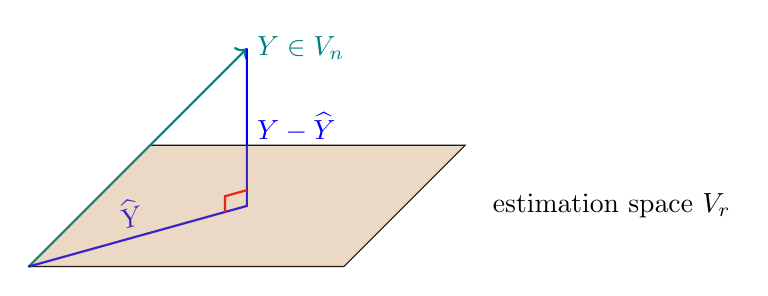
\begin{tikzpicture}[=>stealth]
\draw(0,0,0)--(4,0,0)--(4,0,4)--(0,0,4)--(0,0,0);
\draw[->,thick,teal](0,0,4)--(2,2,2)node[right]{$Y\in V_n$};
\draw[thick,blue](0,0,4)--node[above,sloped]{$\widehat{Y}$}(2,0,2)--node[right]{$Y - \widehat{Y}$}(2,2,2);
\draw[thick,red](1.8,0,2.2)--(1.8,0.2,2.2)--(2,0.2,2);
\path[fill=brown,opacity=0.3](0,0,0)--(4,0,0)--(4,0,4)--(0,0,4)--(0,0,0);
\draw(5,0,2)node[right]{estimation space $V_r$};
\end{tikzpicture}
\end{figure}
\begin{align*}
\widehat{Y} & = X\widehat{B}\\
Y & = X\widehat{B}
\end{align*}


\begin{defn}\label{res:defn:2.3.1}
A matrix whose columns are linearly independent is known as full column rank.\\

Since the mean vector $\big(XB\big)$ of $Y$ lies in the estimation space say $V$ which is spanned by the columns of the design matrix $X$ then the solution in $(**)$ must satisfy $X\widehat{B}=P_vY$, where $P_vY$ is the projection of $Y$ on the space $V$, $P_v$ is known the projection matrix on $V$.
\end{defn}


\begin{thm}\label{res:thm:2.3.2}
If $V$ is the subspace spanned by the linearly independent vectors of the design matrix $X$ i.e $X$ if full column rank matrix then the projection matrix on the space $V$ is $$P_v=X\big(X^tX\big)^{-1}X^t.$$
\end{thm}

\begin{proof}

$P_v^t  = X\big(X^tX\big)^{-1}X^t=P_v$

\begin{align*}
P_v^2 & = P_v\, P_v = X\big(X^tX\big)^{-1}X^tX\big(X^tX\big)^{-1}X^t\\
      & = XI\big(X^tX\big)^{-1}X^t\\
      & = X\big(X^tX\big)^{-1}X^t\\
      & = P_v
\end{align*}
\begin{align*}
X^tX\widehat{B} & = X^tY\\
\big(X^tX\big)^{-1}X^tX\widehat{B} & = \big(X^tX\big)^{-1}X^tY\\
\widehat{B} & = \big(X^tX\big)^{-1}X^tY\\
X\widehat{B} & = X\big(X^tX\big)^{-1}X^tY
\end{align*}
$$\widehat{B} =\big(X^tX\big)^{-1}X^tY$$
$$E\big(\widehat{B}\big)=\big(X^tX\big)^{-1}X^tE(Y)=\big(X^tX\big)^{-1}X^tXB=B$$
\begin{align*}
Cov\big(\widehat{B}\big) & = \big(X^tX\big)^{-1}X^t\Sigma_YX\big(X^tX\big)^{-1},\quad  \Sigma = \sigma^2I\\
                     & = \big(X^tX\big)^{-1}X^t\Sigma X\big(X^tX\big)^{-1}\\
                     & = \big(X^tX\big)^{-1}X^t\sigma^2IX\big(X^tX\big)^{-1}\\
                     & = \sigma^2\big(X^tX\big)^{-1}X^tX\big(X^tX\big)^{-1}\\
                     & = \sigma^2\big(X^tX\big)^{-1}\\
\end{align*}
\end{proof}


\begin{thm}\label{res:thm:2.3.3}
If $Y=XB+\varepsilon\quad  \varepsilon \thicksim N(0,\sigma^2I)$, and $X$ has full column rank $\big(E(Y)=XB,\quad  Cov(Y)=\sigma^2I\big).$
\begin{enumerate}
\item[i.] The least squares estimators of $B$ $\Big(\widehat{B}=\big(X^tX\big)^{-1}X^tY\Big)$ is unbiased.
\item[ii.] $Cov\big(\widehat{B}\big)=\sigma^2\big(X^tX\big)^{-1}$
\item[iii.] $\min||Y-XB||^2$ is achieved when $\widehat{B}=\big(X^tX\big)^{-1}X^tY.$\\
\end{enumerate}
\end{thm}


\begin{proof}
\begin{enumerate}
\item[(i)] and (ii) already
\item[iii).] The minimum of $||Y-XB||^2$ is achieved when $X\widehat{B}$ is the projection of $Y$ on the vector space spanned by the column of $X$. The projection of $Y$ on  the space spanned the column of $X$ is given by $P_vY$ where $P_v=X\big(X^tX\big)^{-1}X^t$, therefore $X\widehat{B}=X\big(X^tX\big)^{-1}X^tY$.
\begin{align*}
X^tX\widehat{B} & = X^tX\big(X^tX\big)^{-1}X^tY=X^tY\\
\big(X^tX\big)^{-1}X^tX\widehat{B} & = \big(X^tX\big)^{-1}X^tY\\
\implies \quad  \widehat{B} & = \big(X^tX\big)^{-1}X^tY\\
\end{align*}
\end{enumerate}
\end{proof}


\begin{thm}[Gauss-Markov theorem]\label{res:thm:2.3.4}
Let $Y=XB+\varepsilon$, be a linear model. If $E(Y)=XB$ and $Cov(Y)=\Sigma_Y$ which is non-singular and $X$ is full column rank then the least squares estimator of $B, \, \widehat{B}=\big(X^tX\big)^{-1}X^tY$ has "minimum variance" within the classes of linear unbiased estimators of $B$ i.e $\widehat{B}$ is BLUE (Best Linear Unbiased Estimator).
\end{thm}


\begin{coro}\label{res:coro:2.3.5}
Let $X=
\begin{pmatrix}
x_1 & x_2 & \cdots & x_k\\
\end{pmatrix}
$ $\big(x_j$ is the $j^{\text{th}}$ column of matrix $X$, $j=1,2,\ldots ,k\big)$ be the design matrix with orthogonal columns $\big($ i.e $x^t_jx_{j'}=0$, if $j\neq j'\big)$, then the least squares estimators of $B$, the components are given $$\widehat{B}_j=\frac{X_j^tY}{X^t_jX_j}=\frac{X^t_jY}{||X_j||^2}\, j=1,2,\ldots ,k\qquad  \text{and they are independent.}$$
\end{coro}


\begin{proof}
\begin{align*}
\underbrace{X^tX}_{k\times k} & =
\begin{pmatrix}
X^t_1X_1 & 0 & \cdots & 0\\
0        & X^t_2X_2 & \cdots & 0\\
\vdots   & \vdots   &   & \vdots\\
0 & 0 & \cdots & X_k^tX_k\\
\end{pmatrix}\\
\big(X^tX\big)^{-1} & = 
\begin{pmatrix}
\frac{1}{X^t_1X_1} & 0 & \cdots & 0\\
0  &\frac{1}{X^t_2X_2} & \cdots & 0\\
\vdots & \vdots & & \vdots\\
\vdots & \vdots & & \vdots\\
0      &   0    & \cdots & \frac{1}{X^t_kX_k} 
\end{pmatrix}\\
\widehat{B} & = \big(X^tX\big)^{-1}X^tY\\
\end{align*}


$j^{\text{th}}$ component of $\widehat{B}$ which is $\widehat{B}_j$\\

$j^{\text{th}}$ row of matrix $\big(X^tX\big)^{-1}X^t$ into $Y$. $$\widehat{B}_j=\frac{X^t_jY}{X_j^tX_j}$$\\


$\bullet$ $\quad  Y_{ij}=\mu_j+\varepsilon_{ij},\quad  \varepsilon_{ij}\thicksim^{iid} N(0,\sigma^2)\quad  i=1,2,\ldots ,n_j$

$$Y=XB+\varepsilon\quad  B=
\begin{pmatrix}
\beta_1 & \beta_2 & \cdots & \beta_4\\
\end{pmatrix}^t\quad  k=4$$
$$
\underbrace{X}_{N\times 4}  =
\begin{pmatrix}
1_{n_1} & 0 & 0 & 0\\
0  & 1_{n_2} & 0 & 0\\
0 & 0 &  1_{n_3} & 0\\
0 & 0 & 0 & 1_{n_4}\\
\end{pmatrix}\qquad ,\qquad 
\underbrace{X^tX}_{4\times 4}  = 
\begin{pmatrix}
n_1 & 0 & 0 & 0\\
0 & n_2 & 0 & 0\\
0 & 0 & n_3 & 0\\
0 & 0 & 0 & n_4\\
\end{pmatrix}
$$
\begin{align*}
\big(X^tX\big)^{-1} & =
\begin{pmatrix}
\frac{1}{n_1} & 0 & 0 & 0\\
0 & \frac{1}{n_2} & 0 & 0\\
0 & 0 & \frac{1}{n_3} & 0\\
0 & 0 & 0 & \frac{1}{n_4}\\
\end{pmatrix}\\
\end{align*}
\begin{align*}
\underbrace{X^t}_{4\times N} & =
\begin{pmatrix}
1^t_{n_1} & 0 & \cdots & 0\\
0 & 1^t_{n_2} & \cdots & 0\\
0 & \cdots & 1^t_{n_3} & 0\\
0 & 0 & \cdots & 1^t_{n_4}\\ 
\end{pmatrix}\\
X^tY & = 
\begin{pmatrix}
1^t_{n_1} & 0 & \cdots & 0\\
0 & 1^t_{n_2} & \cdots & 0\\
0 & \cdots & 1^t_{n_3} & 0\\
0 & 0 & \cdots & 1^t_{n_4}\\
\end{pmatrix}
\begin{pmatrix}
Y^*_1\\ Y^*_2\\ Y^*_3\\ Y^*_4\\
\end{pmatrix}
\end{align*}
$Y^*_j$ observations from the $j^{\text{th}}$ treatment.
\end{proof}


\begin{coro}\label{res:coro:2.3.4}
If $V\thicksim N\big(XB,\sigma^2I\big)$ where $X$ is full column rank, then
\begin{enumerate}
\item[i).] The least squares estimators $\widehat{B}$ is mle of $B$.
\item[ii).] $\widehat{B}\thicksim N\big(B,\sigma^2\big(X^tX\big)^{-1}\big)$.

$$Y=XB + \varepsilon$$
$$\widehat{Y}=X\widehat{B}$$
$$\widehat{\varepsilon} =Y-\widehat{Y}$$
\begin{align*}
\text{SSE}\, = \widehat{\varepsilon}^t\widehat{\varepsilon} & = \big(Y-\widehat{Y}\big)^t\big(Y-\widehat{Y}\big)\\
 & = \big(Y-X\widehat{B}\big)^t\big(Y-X\widehat{B}\big)\\
 & = \big(Y-X\big(X^tX\big)^{-1}X^tY\big)^t\big(Y-X\big(X^tX\big)^{-1}X^tY\big)\\
 & = \big[\big(I-X\big(X^tX\big)^{-1}X^t\big)Y\big]^t\big(\big(I-X\big(X^tX\big)^{-1}X^t\big)Y\big)\\
 & = Y^t\big(I-H\big)^t\big(I-H\big)Y,\quad  H=X\big(X^tX\big)^{-1}X^t\\
 & = Y^t\big(I-H\big)\big(I-H\big)Y\\
 & = Y^t(I-H)Y
\end{align*}
SSE $=Y^t\big(I-H\big)Y$, where $H^2=H=P_v$
$$\text{MSE}=\frac{\text{SSE}}{N-K}=\frac{Y^t\big(I-H\big)Y}{N-K}\thicksim \frac{\chi^2_{N-K}}{N-K}$$\\
\end{enumerate}
\end{coro}


\subsection{Estimability and the Generalized Inverse}

Everything so far has assumed that $X$ has full column rank, so that
$\left(X^tX\right)^{-1}$ exists and the normal equations have one solution.
The analysis of variance models of Section~1 do not satisfy that assumption.
In the one-way layout
$$Y_{ij}=\mu+\tau_j+\varepsilon_{ij},$$
there are $k+1$ parameters $\mu,\tau_1,\dots,\tau_k$ but the design matrix has
rank $k$: its first column is the sum of the others. The normal equations then
have infinitely many solutions, and no amount of data will separate $\mu$ from
the $\tau_j$ --- adding a constant to $\mu$ and subtracting it from every
$\tau_j$ leaves every fitted value unchanged.

This is not a defect to be repaired. It is a statement about which questions
the experiment can answer. Some functions of the parameters are determined by
the data and some are not, and this subsection says exactly which.

\begin{defn}[Generalized inverse]
\label{res:defn:ginv}
A matrix $A^{-}$ is a generalized inverse of $A$ if
$$A A^{-} A = A.$$
When $A$ is non-singular the only such matrix is $A^{-1}$; otherwise $A^{-}$
exists but is not unique.
\end{defn}

\begin{result}
\label{res:result:normalsol}
The normal equations $X^tX\underline{b}=X^t\underline{Y}$ are always
consistent, and every solution has the form
$$\widehat{\underline{b}}=\left(X^tX\right)^{-}X^t\underline{Y}$$
for some generalized inverse $\left(X^tX\right)^{-}$. Different generalized
inverses give different solutions.
\end{result}

\begin{note}
Consistency is the important half: however deficient $X$ may be, a least
squares solution always exists. What fails without full rank is uniqueness,
and uniqueness is not needed for the parts of the answer that matter, as the
next definition makes precise. Note also that the fitted values are unique
regardless, since $X\widehat{\underline{b}}=H\underline{Y}$ with
$H=X\left(X^tX\right)^{-}X^t$ the projection onto the column space of $X$ ---
and a projection does not depend on which generalized inverse produced it.
\end{note}

\begin{defn}[Estimable function]
A linear function $\underline{\lambda}^tB$ of the parameters is
\emph{estimable} if there exists a vector $\underline{a}$ with
$$E\left(\underline{a}^t\underline{Y}\right)=\underline{\lambda}^tB
\qquad\text{for every }B,$$
that is, if some linear function of the observations is an unbiased estimator
of it.
\end{defn}

\begin{thm}[Criterion for estimability]
\label{res:thm:estcrit}
$\underline{\lambda}^tB$ is estimable if and only if
$\underline{\lambda}^t$ lies in the row space of $X$; equivalently, if and
only if
$$\underline{\lambda}^t\left(X^tX\right)^{-}\left(X^tX\right)
=\underline{\lambda}^t .$$
\end{thm}

\begin{proof}
If $\underline{\lambda}^tB$ is estimable then
$\underline{a}^tXB=\underline{\lambda}^tB$ for all $B$, so
$\underline{\lambda}^t=\underline{a}^tX$ and $\underline{\lambda}^t$ is a
combination of the rows of $X$. Conversely if
$\underline{\lambda}^t=\underline{a}^tX$ then
$E\left(\underline{a}^t\underline{Y}\right)=\underline{a}^tXB
=\underline{\lambda}^tB$. The second form follows because
$\left(X^tX\right)^{-}\left(X^tX\right)$ acts as the identity exactly on the
row space of $X$.
\end{proof}

\begin{thm}[Gauss--Markov, rank-deficient form]
\label{res:thm:gmdeficient}
If $\underline{\lambda}^tB$ is estimable then
$\underline{\lambda}^t\widehat{\underline{b}}$ is the same for every solution
$\widehat{\underline{b}}$ of the normal equations, is unbiased for
$\underline{\lambda}^tB$, and has smaller variance than any other linear
unbiased estimator of it. Its variance is
$$\text{Var}\left(\underline{\lambda}^t\widehat{\underline{b}}\right)
=\sigma^2\,\underline{\lambda}^t\left(X^tX\right)^{-}\underline{\lambda}.$$
\end{thm}

\begin{note}
The invariance is the point. A computer package solving a rank-deficient
analysis of variance must pick some generalized inverse, and different
packages pick different ones --- so the printed values of $\widehat{\mu}$ and
$\widehat{\tau}_j$ may differ between two programs run on the same data. The
estimable functions do not differ. If two analyses disagree about a quantity,
that quantity was not estimable, and the disagreement is the software telling
you so.
\end{note}

\begin{exa}
\label{res:exa:estowa}
In the one-way layout with $k$ treatments, write
$B=\left(\mu,\tau_1,\dots,\tau_k\right)^t$. The rows of $X$ are of the form
$\left(1,0,\dots,1,\dots,0\right)$ with the $1$ in position $j+1$, so the row
space consists of all $\underline{\lambda}^t=\left(c,c_1,\dots,c_k\right)$
with $c=\sum_j c_j$. Hence
\begin{itemize}
\item $\mu+\tau_j$ is estimable, with $c=1$, $c_j=1$: it is the mean of
treatment $j$, and $\overline{Y}_{\cdot j}$ estimates it.
\item $\tau_i-\tau_j$ is estimable, with $c=0$: any difference of treatment
effects is estimable, and $\overline{Y}_{\cdot i}-\overline{Y}_{\cdot j}$
estimates it.
\item $\mu$ alone is not estimable: it would need $c=1$ with every $c_j=0$,
and $0\neq1$.
\item $\tau_j$ alone is not estimable, by the same arithmetic.
\end{itemize}
\end{exa}

\begin{note}
Example~\ref{res:exa:estowa} explains why the whole of Section~1 is written in
terms of differences between treatments and never in terms of a single
$\tau_j$. It also puts the familiar side condition $\sum_j\tau_j=0$ in its
place: it is a convention that selects one solution out of the infinitely
many, not information extracted from the data. Imposing it makes $\mu$ and
$\tau_j$ individually computable, but their values then describe the
convention as much as the experiment. Any quantity whose value changes when
the side condition is changed was never estimable.
\end{note}

\begin{defn}[Contrast]
A contrast is an estimable function $\sum_j c_j\tau_j$ with
$\sum_j c_j=0$. Two contrasts $\underline{c}$ and $\underline{d}$ are
orthogonal if $\sum_j c_jd_j/n_j=0$; in the balanced case this is
$\sum_j c_jd_j=0$.
\end{defn}

\begin{note}
By Example~\ref{res:exa:estowa} every contrast is estimable, and the
contrasts are precisely the estimable functions of the $\tau_j$ alone. A set
of $k-1$ mutually orthogonal contrasts partitions $SSTr$ into $k-1$
single-degree-of-freedom sums of squares that add to it exactly --- so a
significant overall $F$ can be followed by an examination of which contrast
carries the effect, with no multiplicity penalty if the contrasts were chosen
before the data were seen.
\end{note}

\subsection{The General Linear Hypothesis}

Individual tests on single parameters have been treated. Most hypotheses of
interest involve several parameters at once: that all treatments are alike,
that a subset of regressors may be dropped, that two effects are equal. All of
them are of one form, and one test covers all of them.

\begin{defn}[General linear hypothesis]
Let $C$ be a $q\times p$ matrix of full row rank whose rows are estimable
functions. The general linear hypothesis is
$$H_0:\ CB=\underline{d}\qquad\text{against}\qquad H_a:\ CB\neq\underline{d}.$$
\end{defn}

\begin{thm}[Test of the general linear hypothesis]
\label{res:thm:glh}
Under $H_0$, with $r=rank(X)$,
$$F=\frac{\left(C\widehat{\underline{b}}-\underline{d}\right)^t
\left[C\left(X^tX\right)^{-}C^t\right]^{-1}
\left(C\widehat{\underline{b}}-\underline{d}\right)\big/q}{MSE}
\ \sim\ F_{q,\,n-r},$$
and $H_0$ is rejected at level $\alpha$ when $F>F_{q,\,n-r,\alpha}$.
\end{thm}

\begin{thm}[Extra sum of squares form]
\label{res:thm:extrass}
The same test is obtained by fitting the model twice. Let $SSE_{\text{full}}$
be the residual sum of squares of the unrestricted model and
$SSE_{\text{red}}$ that of the model fitted subject to $CB=\underline{d}$.
Then
$$F=\frac{\left(SSE_{\text{red}}-SSE_{\text{full}}\right)\big/q}
{SSE_{\text{full}}\big/(n-r)} .$$
\end{thm}

\begin{note}
Theorem~\ref{res:thm:extrass} is the form used in practice, and it is the one
behind every ``extra sum of squares'' calculation in Section~4: the quantity
written $SSR\left(X_2,X_3\mid X_1,X_4\right)$ there is exactly
$SSE_{\text{red}}-SSE_{\text{full}}$ for the hypothesis $\beta_2=\beta_3=0$.
The two theorems are the same test seen from two directions --- one computes
the restriction, the other computes the cost of imposing it. The second needs
no generalized inverse and no matrix $C$, only two model fits, which is why
software reports it that way.
\end{note}

\begin{exa}
For the one-way layout, $H_0:\tau_1=\tau_2=\cdots=\tau_k$ is written with
$q=k-1$ and
$$C=\begin{pmatrix}
0 & 1 & -1 & 0 & \cdots & 0\\
0 & 0 & 1 & -1 & \cdots & 0\\
\vdots & & & \ddots & & \vdots\\
0 & 0 & \cdots & 0 & 1 & -1
\end{pmatrix}.$$
Every row is a contrast, hence estimable, and the resulting $F$ is the
$SSTr/SSE$ ratio of Section~1.2. The reduced model is
$Y_{ij}=\mu+\varepsilon_{ij}$, whose residual sum of squares is $SST$; so
$SSE_{\text{red}}-SSE_{\text{full}}=SST-SSE=SSTr$, as
Theorem~\ref{res:thm:extrass} requires.
\end{exa}

\subsection*{Practice Problems}

\begin{problem}
Show that in the one-way layout $\mu+\overline{\tau}$, where
$\overline{\tau}=\tfrac{1}{k}\sum_j\tau_j$, is estimable, and give a linear
function of the observations that estimates it unbiasedly.
\end{problem}

\begin{problem}
For the randomized block model $Y_{ij}=\mu+\beta_i+\tau_j+\varepsilon_{ij}$,
determine which of $\mu$, $\tau_1$, $\tau_1-\tau_2$, $\beta_1-\beta_2$ and
$\mu+\beta_1+\tau_1$ are estimable.
\emph{Where to start: write down a typical row of $X$ and apply
Theorem~\ref{res:thm:estcrit}.}
\end{problem}

\begin{problem}
Verify Definition~\ref{res:defn:ginv} for
$A=\begin{pmatrix}1&1\\1&1\end{pmatrix}$ by exhibiting two different
generalized inverses, and confirm that $\underline{\lambda}^t=(1,-1)$ gives
the same value of $\underline{\lambda}^tA^{-}\underline{\lambda}$ for both
while $\underline{\lambda}^t=(1,0)$ does not.
\end{problem}

\begin{problem}
With $k=4$ treatments, write down three mutually orthogonal contrasts and
verify their orthogonality. Explain what each one tests if the treatments are
four doses of a fertiliser, $0,1,2,3$ units.
\end{problem}

\begin{problem}
Two statistical packages fit the same one-way analysis of variance and report
different values of $\widehat{\tau}_1$ but identical values of
$\widehat{\tau}_1-\widehat{\tau}_2$ and identical analysis of variance tables.
Explain, and say which of the reported quantities you would be willing to put
in a report.
\end{problem}

\begin{problem}
Show that the hypothesis $\beta_2=\beta_3=0$ in a regression on
$X_1,X_2,X_3,X_4$ can be written as $CB=\underline{0}$, give $C$, and state
the degrees of freedom of the resulting $F$ test.
\end{problem}

\newpage
\subsection{Simultaneous Confidence Intervals and Multiple Comparison}


\textbf{One-dimensional case}\\
Let $C$ be a known $K\times 1$ vector of constants. We want a $100(1-\alpha)\%$ confidence interval for $\underbrace{C^t}_{1\times K}\underbrace{B}_{K\times 1}$.\\ Let $\text{MSE}=\frac{Y^t\big(I-H\big)Y}{N-K}$, mean squared error then $\hat{B}$ the least squares estimator of $B$ in the linear model $$Y=XB+\varepsilon,\quad  E(\varepsilon)=0,\quad  Cov(\varepsilon)=\sigma^2I$$
$X$ to be full column rank matrix. $\hat{B}$ and MSE are independent (probability) since there are functions of projections onto orthogonal spaces.\\


% DIAGRAM M
\begin{figure}[H]
\centering
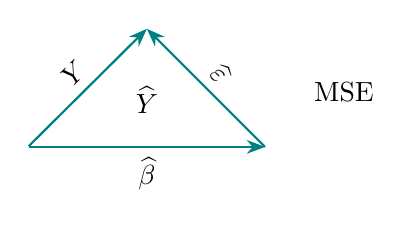
\begin{tikzpicture}[=>stealth]
\draw[-Stealth,teal,thick](0,0)--node[below,sloped,black]{$\widehat{\beta}$}(3,0);
\draw[-Stealth,thick,teal](0,0.01)--node[above,sloped,black]{$Y$}(1.5,1.5);
\draw[-Stealth,teal,thick](3,0)--node[above,sloped,black]{$\widehat{\varepsilon}$}(1.5,1.5);
\draw(1.5,0.3)node[above]{$\widehat{Y}$}
(3.5,0.7)node[right]{\text{MSE}};
\end{tikzpicture}
\end{figure}


$$\widehat{B}\thicksim N\big(B,\sigma^2\big(X^tX\big)^{-1}\big)$$
\begin{align*}
C^tB & \thicksim \Big(C^tB,C^tCov\big(\widehat{B}\big)C\Big)\\
     & \thicksim N\Big(C^tB, C^t\sigma^2\big(X^tX\big)^{-1}C\Big)\\
     & \thicksim N\Big(C^tB, \sigma^2\underbrace{C^t}_{1\times k}\underbrace{\big(X^tX\big)^{-1}}_{k \times k} \underbrace{C}_{k\times 1}\Big)
\end{align*}
\begin{align*}
\frac{C^t\widehat{B}-C^tB}{\sqrt{\sigma^2C^t\big(X^tX\big)^{-1}C}} & \thicksim N(0,1)\\
\frac{C^t\widehat{B}-C^tB}{\sqrt{\text{MSE}\, C^t\big(X^tX\big)^{-1}C}} & \thicksim t_{N-K}\\
\end{align*}


$\therefore$ The $100(1-\alpha)\%$ C.I for $C^tB$ is $$C^t\widehat{B}\pm t_{\frac{\alpha}{2},N-K}\sqrt{\text{MSE}\,C^t\big(X^tX\big)^{-1}C}$$

\begin{enumerate}
\item[a).] If we want $100(1-\alpha)\%$ for $\beta_j$\\

Let $C=
\begin{pmatrix}
0 & 0 & \cdots & 0 & 1 & 0 & \cdots\\
\end{pmatrix}^t
,\quad  C^tB=\beta_j$.\\

$\widehat{\beta}_j\pm t_{\frac{\alpha}{2},N-K}\sqrt{\text{MSE}\,C^t\big(X^tX\big)^{-1}C}$, $j^{\text{th}}$ diagonal element of $\big(X^tX\big)^{-1}_{jj}$.

\item[b).] If we want $100(1-\alpha)\%$ C.I for $\beta_j-\beta_{j'},\, j\neq j'$.\\

Let $C-$ should be such that it has 1 on the $j^{\text{th}}$ position, $-1$ on the $j'^{\text{th}}$ position and zeroes elsewhere. If we assume $j<j'$
$$C=
\begin{pmatrix}
0 & 0 & \cdots & \underbrace{1}_{j} & 0 &\cdots & \underbrace{-1}_{j'} & \cdots & 0\\
\end{pmatrix}^t
$$
$100(1-\alpha)\%$ C.I for $\beta_j-\beta_{j'}$ is given by 
$$C^t\widehat{B}\pm t_{\frac{\alpha}{2},N-K}\sqrt{\text{MSE}\,C^t\big(X^tX\big)^{-1}C}$$\\
\end{enumerate}


\begin{thm}\label{res:thm:2.4.1}
Let $\widehat{B}$ be the least squares estimators of $B$, $X$ the design matrix full column rank and MSE mean squared error with $N-K$ df, for the linear model $$Y=XB+\varepsilon,\quad  E(\varepsilon)=0,\quad  Cov(\varepsilon)=\sigma^2I$$

\begin{enumerate}
\item[i).] $\displaystyle{ \frac{\big(\widehat{B}-B\big)^tX^tX\big(\widehat{B}-B\big)}{\sigma^2}\thicksim \chi^2_K}$\\

\item[ii).] $\displaystyle{\frac{\big(\widehat{B}-B\big)^tX^tX\big(\widehat{B}-B\big)}{K\,\text{MSE}}\thicksim f_{K,N-K}}$\\

$$=\frac{\big(\hat{B}-B\big)^tX^tX\big(\hat{B}-B\big)}{K\sigma^2}\Bigg/\frac{\text{MSE}}{\sigma^2}=\frac{\text{SSE}}{N-K\sigma^2}\bigg/N-K$$
$$=\frac{\frac{\chi^2_K}{K}}{N-K\cdot\frac{\chi^2_{N-K}}{N-K}}$$\\
\end{enumerate}
 
 
 
 
\begin{enumerate}
\item[\textbf{Remark 1:}]
 If we know the "nuisance parameter" $\sigma^2$ we would get our confidence set based on the Chi-square i.e $$\Bigg\{B^*:\frac{\big(\widehat{B}-B^*\big)^tX^tX\big(\widehat{B}-B^*\big)}{\sigma^2}\leq \chi^2_{k,\alpha}\Bigg\}$$ would be the $(100-\alpha)\%$ confidence set for $B$.
 
 
\item[\textbf{Remark 2:}]
 The $100(1-\alpha)\%$ confidence set for $B$ is given $$\Bigg\{B^{\thicksim}:\frac{\big(\widehat{B}-B^{\thicksim}\big)^tX^tX\big(\widehat{B}-B^{\thicksim}\big)}{K\,\text{MSE}}\leq f^{\alpha}_{K,N-K}\Bigg\}$$
\end{enumerate}
The confidence sets are ellipsoids in $K-$ dimensional space. It is difficult to visualize $B$ in an ellipsoid but it is easy to think of $\beta_j$ in some interval $[a_j,b_j]$ $,\, j=1,2,\ldots ,k$\\

hence the simultaneous confidence intervals\\

% DIAGRAM 4
\begin{figure}[H]
\centering
\begin{tikzpicture}[=>stealth]
\draw[->](-1,0)--(4,0)node[right]{$\beta_1$};
\draw[->](0,-1)--(0,4)node[above]{$\beta_2$};
\draw(1,0)node[below]{$a_1$}
(3,0)node[below]{$b_1$}
(0,1)node[left]{$a_2$}
(0,3)node[left]{$b_2$};
\draw[rotate = 45,teal](2,0.3)ellipse[x radius =1, y radius = 0.5];
\end{tikzpicture}
\end{figure}



\end{thm}

\subsection*{Simultaneous Confidence Intervals}


\textbf{Using Bonferroni's Inequality}\\

For any events $A_1, A_2,\ldots , A_k$ $$P\Bigg(\bigcup^k_{j=1}A_j\Bigg)\leq \sum^k_{j=1}P\big(A_j\big).$$ This inequality is known as Bonferroni's inequality. Applying this inequality to confidence intervals we have the next Lemma.\\

\begin{itemize}
\item[]\textbf{Step 1:} Check if it is true for $n\geq a$, here $n=2$.
\item[]\textbf{Step 2:} Assume it is true for $n=k$.
\item[]\textbf{Step 3:} Show that if it is true for $n=k$ then it is true for $n=k+1$\\
\end{itemize}


\begin{proof}
\begin{enumerate}
\item $P\big(A_1\cup A_2\big)=P(A_1)+P(A_2)-P(A_1\cap A_2)$
\item $P\Bigg(\bigcup\limits^k_{j=1}A_j\Bigg)\leq \displaystyle{\sum^k_{j=1}P(A_j)}$
\item We show that $\displaystyle{P\Bigg(\bigcup^{k+1}_{j=1}A_j\Bigg)\leq \sum^{k+1}_{j=1}P(A_j)}$
\begin{align*}
\text{L.H.S}\quad  P\Bigg(\bigcup^{k+1}_{j=1}A_j\Bigg) & = P\Bigg(\bigg(\bigcup^k_{j=1}A_j\big)\cup A_{k+1}\Bigg)\\
                                                               & = P(D)+P(A_{k+1})-P(D\cup A_{k+1}),\quad  D=\bigcup^k_{j=1}A_j\\
                                                               &\leq \sum^k_{j=1}P(A_j)+P(A_{k+1})-P(D\cap A_{k+1})\\
                                                               & \leq \sum^{k+1}_{j=1}P(A_j)\\
\end{align*}
\end{enumerate}
\end{proof}


\begin{lem}\label{res:lem:2.3.2}
Let $I_j(Y)$ be a $100(1-\alpha)\%$ confidence interval for the parameter $\gamma_j,\, j=1,2,\ldots ,k$. The probability that all $k$ intervals simultaneously contain their parameter is greater than or equal to $$1-\sum^k_{j=1}\alpha_j\quad \text{i.e}\quad  P\Bigg\{\bigcap^k_{j=1}\Big(\gamma_j\in I_j(Y)\Big)\Bigg\}\geq 1-\sum^k_{j=1}\alpha_j$$
\end{lem}

\begin{proof}
Apply the Bonferroni's Inequality.
\begin{align*}
P\Big\{\bigcap^k_{j=1}\big(\gamma_j\in I_j(Y)\big)\Big\} & = 1- P\Big\{\bigcap^k_{j=1}\big(\gamma_j\in I_j(Y)\big)\Big\}^c\\
                                                         & = 1 -P\Big\{\bigcup^k_{j=1}\big(\gamma_j\not\in I_j(Y)\big)\Big\}\\
 \therefore P\Bigg(\bigcap^k_{j=1}\big(\gamma_j\in I_j(Y)\big)\Bigg) & \geq 1-\sum^k_{j=1}\alpha_j                                                        
\end{align*}
Usually $\alpha_{j'}$s are all equal. Thus if we want simultaneous $100(1-\alpha)\%$ C.Is of $\beta_{j'}$s we set $$\alpha_j=\frac{\alpha}{k}$$
\end{proof}


\begin{defn}\label{res:defn:2.3.3}
\begin{enumerate}
\item A contrast of parameters $\beta_1,\beta_2,\ldots ,\beta_k$ is a linear combination of the parameter with coefficients adding up to zero $$\text{i.e}\quad  \sum^k_{j=1}C_j\beta_j=C^tB$$ such that $\sum\limits^k_{j=1}C_j=0$.
\item A simple contrast is a contrast such that there are only two non-zero elements of the vector $C$, a one (1) and a minus one $(-1)$. $$\text{i.e}\quad  \beta_1-\beta_2=C^tB,\quad  C^t=
\begin{pmatrix}
1  & -1 & 0 & \cdots & 0\\
\end{pmatrix}
$$
$\beta_j-\beta_{j'}=C^tB,\quad  C$ has one(1) in the $j^{\text{th}}$ position and minus one $(-1)$ in the $j'^{\text{th}}$ position.\\
\end{enumerate}
\end{defn}


\begin{exa}\label{res:exa:2.3.4}
Suppose in  a linear model $$Y=XB+\varepsilon$$ $Y$ is $15\times 1$, $\quad  X$ is $15\times 3$, $\quad  B$ is $3\times 1$, $\quad \varepsilon$ is $15\times 1$,
$$X=
\begin{pmatrix}
1_5 & 0 & 0\\
0 & 1_5 & 0\\
0 & 0 & 1_5\\
\end{pmatrix}
\,,\quad  \widehat{B}=
\begin{pmatrix}
29.4 & 29.6 & 28.0\\
\end{pmatrix}^t
\,, \quad  \text{MSE} = 9.7$$

\begin{enumerate}
\item
\begin{enumerate}
       \item Find $95\%$ C.I for $\beta_2$.
       \item Find $95\%$ C.I for $\beta_3-\beta_1$.
       \item Find $95\%$ C.I for $\frac{\beta_1+\beta_2+\beta_3}{3}$.
\end{enumerate}

\item
\begin{enumerate}
     \item Simultaneous C.Is for $\beta_1,\beta_2,\beta_3$.
     \item Simultaneous C.I for all the simple contrasts.\\
\end{enumerate}
\end{enumerate}
\end{exa}


\begin{solution}

$$\widehat{B}=
\begin{pmatrix}
29.4 & 29.6 & 28.0\\
\end{pmatrix}^t
\,, \quad  \text{MSE} = 9.7\, ,\quad  X^tX=
\begin{pmatrix}
5 & 0 & 0\\
0 & 5 & 0\\
0 & 0 & 5\\
\end{pmatrix}
$$

\begin{enumerate}
\item
\begin{enumerate}
    \item $95\%$ C.I for $\beta_2$
\begin{align*}
\widehat{\beta}_2 & \pm t^{0.05}_{12}\,\sqrt{\text{MSE}\,\big(X^tX\big)^{-1}_{22}}\\
29.6 & \pm 2.179\sqrt{9.7\times \frac{1}{5}}\\
\end{align*}

     \item $95\%$ C.I for $\beta_3-\beta_1$
\begin{align*}
\widehat{\beta}_3-\widehat{\beta}_1 & \pm t^{0.05}_{12}\sqrt{\text{MSE}\,C^t\big(X^tX\big)^{-1}C}\quad ,\quad  C=
\begin{pmatrix}
-1 & 0 & 1\\
\end{pmatrix}^t\\
28.0-29.4 & \pm 2.179\sqrt{9.7\times \big(\frac{1}{5}+\frac{1}{5}\big)}\\
\end{align*}

       \item $95\%$ C.I for $\frac{\beta_1+\beta_2+\beta_3}{3}$
\begin{align*}
\frac{\widehat{\beta}_1+\widehat{\beta}_2+\widehat{\beta}_3}{3} & \pm t^{0.05}_{12}\sqrt{\text{MSE}\, C^t\big(X^tX\big)^{-1}C}\qquad  C=
\begin{pmatrix}
\frac{1}{3} & \frac{1}{3}&\frac{1}{3}\\
\end{pmatrix}^t\\
\frac{29.4+29.6+28.0}{3} & \pm 2.179\sqrt{9.7\times \frac{3}{9\times 5}}\\
\end{align*} 
\end{enumerate}

\item
\begin{enumerate}
      \item Simultaneous $94\%$ C.I for $$\widehat{\beta}_1,\quad \widehat{\beta}_2,\quad  \widehat{\beta}_3,\qquad  \frac{\alpha}{3}=\frac{0.06}{3}=0.02$$
\begin{align*}
\beta_1 :\quad  &  \widehat{\beta}_1 \pm t^{0.01}_{12}\sqrt{\text{MSE}\,\big(X^tX\big)^{-1}_{11}}\\
          & 29.4\pm 2.68\sqrt{9.7\times \frac{1}{5}}
\end{align*}
\begin{align*}
\beta_2 :\quad  & \widehat{\beta}_2 \pm t^{0.01}_{12}\sqrt{\text{MSE}\,\big(X^tX\big)^{-1}_{22}}\\
          & 29.6 \pm 2.68 \sqrt{9.7\times \frac{1}{5}}
\end{align*}
\begin{align*}
\beta_3 :\quad  & \widehat{\beta}_3 \pm t^{0.01}_{12}\sqrt{\text{MSE}\,\big(X^tX\big)^{-1}_{33}}\\
          & 28.0 \pm 2.681\sqrt{9.7\times \frac{1}{5}}\\
          & 28.0 \pm 3.696\\
\end{align*}

         \item $94\%$ simultaneous for all the simple contrast $$\widehat{\beta}_1-\widehat{\beta}_2,\quad  \widehat{\beta}_1-\widehat{\beta}_3,\quad  \widehat{\beta}_2-\widehat{\beta}_3$$ 
         $$\frac{\alpha}{2}=\frac{0.06}{3}=0.02$$
\begin{align*}
\beta_1-\beta_2:\quad  & \widehat{\beta}_1-\widehat{\beta}_2 \pm t^{0.01}_{12}\sqrt{\text{MSE}\,C^t\big(X^tX\big)^{-1}C}\\
                 & 29.4-29.6 \pm 2.68\sqrt{9.7\times \frac{2}{5}}\,,\quad  C=
\begin{pmatrix}
1 & -1 & 0\\
\end{pmatrix}^t
\end{align*}
\begin{align*}
\beta_1-\beta_3:\quad  & \widehat{\beta}_1-\widehat{\beta}_3 \pm t^{0.01}_{12}\sqrt{\text{MSE}\,C^t\big(X^tX\big)^{-1}C}\\
                 & 29.4-28.0 \pm 2.681\sqrt{9.7\times \frac{2}{5}}\,,\quad  C=
\begin{pmatrix}
1 & 0 & -1\\
\end{pmatrix}^t
\end{align*}
\begin{align*}
\beta_2-\beta_3 :\quad  & 29.6-28.0 \pm 2.681\sqrt{9.7\times \frac{2}{5}}\\
                  & (29.6-28.0)\pm 5.281\\
\end{align*}
\end{enumerate}
\end{enumerate}
\end{solution}


\subsection*{Simultaneous Confidence Intervals by Scheff\'e's Method}

\begin{thm}\label{res:thm:2.3.5}
Let $\widehat{B}$ be the least square estimator for $B$ in the linear model $Y=XB+\varepsilon$, $\quad  \varepsilon \thicksim N(0,I\sigma^2)$, then the $100(1-\alpha)\%$ confidence interval for $C^tB$ is given by $$C^t\widehat{B}\pm \sqrt{Kf^{\alpha}_{K,N-K}}\sqrt{\text{MSE}\,C^t\big(X^tX\big)^{-1}C}$$ for all vectors $C$.\\


\begin{note}
The length of the interval depend on the number of  components of $B$ and not on the number of intervals like the  simultaneous confidence interval using the Bonferroni's method.
\end{note}
$$K=5,\quad  \beta_j-\beta_{j'},\quad  i=j'$$
\end{thm}


\begin{exa}\label{res:exa:2.3.6}

Data: $\widehat{B}=
\begin{pmatrix}
29.4 & 29.6 & 28.0\\
\end{pmatrix}^t
$
$$\text{MSE} = 9.7\, ,\quad  df=12\, ,\quad  X^tX =5I_3$$

Find $95\%$ simultaneous C.Is for $\beta_1, \beta_2, \beta_3$ using S-method. $$K=3,\quad  N-K=12$$
\begin{align*}
\beta_1:\quad  & \widehat{\beta}_1 \pm \sqrt{Kf^{\alpha}_{K,N-K}}\sqrt{\text{MSE}\,\big(X^tX\big)^{-1}_{11}}\\
         & 29.4 \pm \sqrt{3f^{0.05}_{3,12}}\sqrt{9.7\times \frac{1}{5}}\\
         & 29.4\pm \sqrt{3\times 3.49}\sqrt{\frac{9.7}{5}}
\end{align*}
\begin{align*}
\beta_2:\quad  & 29.6 \pm \sqrt{3\times 3.49}\sqrt{9.7/5}
\end{align*}
\begin{align*}
\beta_3:\quad  & 28.0 \pm \sqrt{3\times 3.49}\sqrt{9.7/5}\\
\end{align*}
\end{exa}


\begin{exa}\label{res:exa:2.3.7}
In a study of effectiveness of different rust inhibitors, four brands $A,B,C$ and $D$ were tested, each on a different set of five units. The basic results were 

\begin{table}[h!]
\centering
\begin{tabular}{c|cccc}
inhibitor & $A$ & $B$ & $C$ & $D$\\
\hline
mean & 43 & 89 & 67 & 40\\
\end{tabular}
\end{table}

The higher the value the more effective the rust inhibitor.\\

The error sum of squares is 72. Find $95\%$ simultaneous C.Is of the individual parameters together with all the simple contrasts, using Bonferroni and S-method

\begin{enumerate}
\item Bonferroni
$$\alpha = 0.05,\quad  \text{MSE} = \frac{72}{16},\quad  10\implies \frac{\alpha}{10}=0.005$$
$$\beta_j : \hat{\beta}_j \pm t^{0.005}_{16}\sqrt{4.5\times \frac{1}{5}}$$
$$\hat{\beta}_j\pm 3.252\sqrt{4.5\times \frac{1}{5}}$$
$$\beta_j-\beta_{j'}: \hat{\beta}_j-\hat{\beta}_{j'}\pm 3.252\sqrt{4.5\times \frac{2}{5}}$$



\item S-Method
\begin{align*}
\beta_j:\quad  & \widehat{\beta}_j \pm \sqrt{Kf^{0.05}_{K,N-K}}\,\sqrt{\text{MSE}\,\cdot \frac{1}{n}}\\
         &  \widehat{\beta}_j \pm \sqrt{4f^{0.05}_{4,16}}\,\sqrt{4.5\times \frac{1}{5}}\\
           & \widehat{\beta}_j \pm \sqrt{4\times 3.06}\,\sqrt{4.5\times \frac{1}{5}}
\end{align*}
$$\beta_j-\beta_{j'}:\quad  \widehat{\beta}_j-\widehat{\beta}_{j'} \pm \sqrt{4\times 3.06}\,\sqrt{4.5\times \frac{2}{5}}$$

$\bullet$ Bonferroni is better method for confidence interval than the S-method.\\
\end{enumerate} 
\end{exa}


\subsection*{Tukey Method of Multiple Comparison}
The Tukey method of multiple comparison we will consider applies when the interest is only the pairwise simple contrasts.\\


\textbf{Studentized range Distribution}\\
The Tukey method utilizes the studentized range distribution. Let $Y_1, Y_2,\ldots , Y_k$ be independent observations from $N(\mu,\sigma^2)$ and $W$ be the range of this set of  observations i.e $$W=\max\big\{Y_1,Y_2,\ldots ,Y_k\big\}-\min\big\{Y_1,Y_2,\ldots ,Y_k\big\}$$ Let $S^2$ be the estimate of $\sigma^2$ based on $v$ degrees of freedom and is independent of the $Y_{j'}$s, then the ratio $W/S$ is called studentized range as is denoted by $$l(k,v)=\frac{W}{S}$$


\subsection*{Multiple Comparison Confidence Intervals}
The tukey multiple comparison C.Is for all simple contrasts $\beta_j-\beta_{j'}\quad j<j'$ with confidence coefficients of $1-\alpha$ given by 
$$\widehat{\beta}_j-\widehat{\beta}_{j'}\pm \frac{1}{\sqrt{2}}\, l_{(1-\alpha,k,v)} \,\sqrt{\text{MSE}\,\Big(\frac{1}{n_j}+\frac{1}{n_{j'}}\Big)}$$
\begin{itemize}
\item[] $n_j=$ number of  observations for the $j^{\text{th}}$ $+ve$.
\item[] $n_{j'}=$ number of observations for $j'^{\text{th}}$ $+ve$.
\end{itemize}

$$n_j=n\quad  \widehat{\beta}_j-\widehat{\beta}_{j'} \pm l_{(1-\alpha,k,v)}\,\sqrt{\frac{\text{MSE}}{n}}$$


What is $\widehat{\beta}_j$ for one-way ANOVA? \quad $\widehat{\beta}_j=\overline{Y}._j$


\begin{exa}\label{res:exa:2.3.8}
Same data as in Example~\ref{res:exa:2.3.7}\\

\begin{table}[h!]
\centering
\begin{tabular}{c|cccc}
Inhibitors & $A$ & $B$ & $C$ & $D$\\
\hline
Means & 43 & 89 & 67 & 40\\
\end{tabular}
\end{table}

$$\text{SSE} = 72\, ,\quad  v=16\,, \quad  X^tX=5I_4$$
$95\%$ Simultaneous C.I for all simple contrasts.

\begin{align*}
\beta_j-\beta_{j'} :\quad  & \widehat{\beta}_j-\widehat{\beta}_{j'}\pm l(0.95,4,16)\,\sqrt{\frac{4.5}{5}}\\
                     & \overline{Y}._j-\overline{Y}._{j'}\pm 4.05\,\sqrt{\frac{4.5}{5}}\\
\end{align*}
\end{exa}


\subsection{Two-Factor Studies}
The RBD is a one-factor study, the interest is on one factor the treatments. The blocks are used because  of not having enough homogeneous experimental units.\\
Two-factors, where factor $A$ has $a-$levels, factor $B$ has $b-$levels.\\

Then we have $ab$ treatments.\\

The Model 

$$Y_{ijl}=\mu_{ij}+\varepsilon_{ijl},\quad  \varepsilon_{ijl}\thicksim^{iid}(0,\sigma^2)$$
$$i=1,2,\ldots ,a\quad  j=1,2,\ldots ,b\quad  l=1,2,\ldots ,n$$
Total number of observations $abn$

$$\widehat{\mu}_{ij}=\overline{Y}_{ij}.\quad  \sum^a_{i=1}\sum^b_{j=1}\sum^n_{l=1}\big(Y_{ijl}-\mu_{ij}\big)^2$$
$$\text{SSE} = \sum \sum \sum \big(Y_{ijl}-\overline{Y}_{ij}.\big)^2$$

\begin{itemize}
\item[] $df=ab(n-1)=$ total number of observations $-$ parameters.
\item[] $Y_{ijl}= l^{\text{th}}$ observation under $i^{\text{th}}$ level of factor $A$ and $j^{\text{th}}$ level of factor $B$.
\item[] $\mu_{ij}=$ the expected mean of the treatment corresponding to the $i^{\text{th}}$ level of factor $A$ and $j^{\text{th}}$ level of factor $B$.
\item[] $\overline{Y}_{ij}.=\frac{1}{n}\sum\limits^n_{l=1}Y_{ijl}=$ sample mean for the $i^{\text{th}}$ level of factor $A$ and $j^{\text{th}}$ level of factor $B$.
\item[] $\overline{Y}_i..=\frac{1}{nb}\sum\limits^b_{j=1}\sum\limits^n_{l=1}Y_{ijl}=$ Sample mean for the $i^{\text{th}}$ level for factor $A$.
\item[] $\overline{Y}._j.=\frac{1}{na}\sum\limits^a_{i=1}\sum\limits^n_{l=1}Y_{ijl}= $ Sample mean for the $j^{\text{th}}$ level of factor $B$.
\item[]$\overline{Y}...=\frac{1}{nab}\sum\limits^a_{i=1}\sum\limits^b_{j=1}\sum\limits^n_{l=1}Y_{ijl}=$ Sample mean\\
\end{itemize}


Let $\displaystyle{Q(Y)=\sum^a_{i=1}\sum^b_{j=1}\sum^n_{l=1}\big(Y_{ijl}-\mu_{ij}\big)^2}$ the least squares estimators for $\mu_{ij'}$s are $\overline{Y}_{ij'}$s.

$$e_{ijl}=Y_{ijl}-\overline{Y}_{ij}.$$

\begin{itemize}
\item[]$\text{SST}=\displaystyle{\sum^a_{i=1}\sum^b_{j=1}\sum^n_{l=1}\big(Y_{ijl}-\overline{Y}...\big)^2}\quad $ Corrected total sum of squares.
\item[]$\text{SSTrt} = \displaystyle{n\sum^a_{i=1}\sum^b_{j=1}\big(\overline{Y}_{ij}.-\overline{Y}...\big)^2}\quad $ Treatment sum of squares.
\item[]$\text{SSE} = \displaystyle{\sum^a_{i=1} \sum^b_{j=1} \sum^n_{l=1} \big(Y_{ijl}-\overline{Y}_{ij}.\big)^2}\quad $ Error sum of squares.\\
\end{itemize}


$$\underbrace{\text{SST}}_{abn-1} = \underbrace{\text{SSTrt}}_{ab-1}+\underbrace{\text{SSE}}_{ab(n-1)}$$
$$Y_{ijl}-\overline{Y}... = \overline{Y}_{ij}.-\overline{Y}...+Y_{ijl}-\overline{Y}_{ij}.$$


\begin{table}[H]
\centering
ANOVA Table\\
\begin{tabular}{|c|ccc|}
\hline
Source of & SS & df & MS\\
Variation &    &    & \\
\hline
&&&\\
Treatment & SSTrt & $ab-1$ & MSTrt $=\frac{\text{SSTrt}}{ab-1}$\\
&&&\\
Error & SSE & $ab(n-1)$ & MSE $=\frac{\text{SSE}}{ab(n-1)}$\\
\hline
Total & SST & $abn-1$ & \\
&&&\\
\hline 
\end{tabular}
\end{table}


Under $H_0:$ the means are all equal (all the treatments are the same)$$H_0:\mu_{11}=\mu_{12}=\mu_{21}=\cdots \mu_{ab}$$
$$\frac{\text{MSTrt}}{\text{MSE}}\thicksim f_{ab-1,ab(n-1)}$$

Reject $H_0$ if $\displaystyle{\frac{\text{MSTrt}}{\text{MSE}}\geq f^{\alpha}_{ab-1,ab(n-1)}}$

$$Y_{ijl} = \mu + \alpha_i +\beta_j + (\alpha\beta)_{ij} + \varepsilon_{ijl}$$
$$\mu = \overline{Y}... \quad  \alpha_i=\overline{Y}_i..-\overline{Y}... \quad \beta_j= \overline{Y}.j.-\overline{Y}...\quad  (\alpha\beta)_{ij}= \underbrace{\overline{Y}_{ij}.-\overline{Y}_i..-\overline{Y}._j.-\overline{Y}...}_{\text{interaction}}$$
$$\varepsilon_{ijl}=Y_{ijl}-\overline{Y}_{ij}.$$
$$\text{SST} = \underbrace{\text{SSA} + \text{SSB} + SS(AB)}_{\text{SSTrt}}+ \text{SSE}$$
$$Y_{ijl} = \mu_{il}+\varepsilon_{ijl},\quad  \varepsilon_{ijl}\thicksim^{iid}N(0,\sigma^2)$$ $$i=1,2,\ldots , a\qquad  j=1,2,\ldots ,b\qquad  l=1,2,\ldots , n$$
\begin{align*}
Y & = XB +\varepsilon\\
Y_{ab\times 1} & = 
\begin{pmatrix}
Y_{111} & Y_{121} & Y_{122} & \cdots & Y_{abn}\\ 
\end{pmatrix}^t\\
\varepsilon_{ab\times 1} & = 
\begin{pmatrix}
e_{111}& \cdots & \cdots & \\
\end{pmatrix}^t\\
B_{ab\times 1} & = 
\begin{pmatrix}
\mu_{11} & \cdots & \mu_{ab}\\
\end{pmatrix}^t
\end{align*}
$$\underbrace{X}_{abn\times ab}=
\begin{pmatrix}
\mu_{11} & \mu_{12} & \mu_{13} & \cdots & \mu_{ab}\\
1_n & 0 & 0 &   & 0\\
0   & 1_n & 0 &  & 0\\
0   &   0 & 1_n &\cdots & 0\\
\vdots & \vdots & \vdots & &\vdots\\
0 & 0 & 0 & \cdots & 1_n\\
\end{pmatrix}
$$
$$Y_{ijl}=\mu + \alpha_i + \beta_j + (\alpha \beta)_{ij} + \varepsilon_{ijl}\qquad  i=1,2,\ldots ,a$$
$$\sum \alpha_i=\sum \beta_j =\sum_i (\alpha\beta)_{ij}=\sum_j(\alpha\beta)_{ij}=0$$


\begin{table}[h!]
\centering
\begin{tabular}{cc}
Parameter & Estimator\\
$\mu$ & $\overline{Y}..$\\
$\alpha_i$ & $\overline{Y}_i..-\overline{Y}...$\\
$\beta_j$ & $\overline{Y}._j.-\overline{Y}...$\\
$(\alpha\beta)_{ij}$ & $\overline{Y}_{ij}.-\overline{Y}_i..-\overline{Y}._j.+\overline{Y}...$\\
\end{tabular}
\end{table}


$$Y_{ijl} -\overline{Y}... = \overline{Y}_i..-\overline{Y}...+\overline{Y}._j.-\overline{Y}...+\overline{Y}_{ij}.-\overline{Y}_i..-\overline{Y}._j.+\overline{Y}...+Y_{ijl}-\overline{Y}_{ij}.\quad  *$$

squaring both sides of $*$ and summing we get 

$$SST = \underbrace{SSA + SSB + SS(AB)}_{SSTrt}+SSE$$
\begin{align*}
SSTrt & = n\sum^a_{i=1}\sum^b_{j=1}\big(\overline{Y}_{ij}.-\overline{Y}...\big)^2\\
      & = \underbrace{bn\sum^a_{i=1}\big(\overline{Y}_i..-\overline{Y}...\big)^2}_{SSA}+\underbrace{an\sum^b_{j=1}\big(\overline{Y}.j.-\overline{Y}...\big)^2}_{SSB}+ \underbrace{n\sum^a_{i=1}\sum^b_{j=1}\big(\overline{Y}_{ij}.-\overline{Y}_i..-\overline{Y}._j.+\overline{Y}...\big)^2}_{SS(AB)}
\end{align*}


\begin{table}[H]
\centering
ANOVA TABLE\\
\begin{tabular}{|c|c|c|c|c|}
\hline
Source of & SS & df & MS & F \\
Variation &&&&\\
\hline
&&&&\\
Factor $A$ & $SSA$ & $a-1$ & $MSA = \frac{SSA}{a-1}$ & $\frac{MSA}{MSE}\thicksim f_{a-1,ab(n-1)}$\\
&&&& $H_0:\alpha_i=0, i=1,2,\cdots,a$\\
&&&&\\
Factor $B$ & $SSB$ & $b-1$ & $MSB=\frac{SSB}{b-1}$ & $\frac{MSB}{MSE}\thicksim f_{b-1,ab(n-1)}$\\
&&&& $H_0:\beta_j=0, j=1,2,\cdots,b$\\
&&&&\\
Interaction & $SS(AB)$ & $(a-1)(b-1)$ & $MS(AB)=\frac{SS(AB)}{(a-1)(b-1)}$ & $\frac{MS(AB)}{MSE}\thicksim f_{(a-1)(b-1),ab(n-1)}$\\
&&&& $H_0:(\alpha\beta)_{ij}=0, i=1,2,\cdots,a$\\
of $A$ and $B$ &&&& $j=1,2,\cdots,b$\\
&&&&\\
Error & $SSE$ & $ab(n-1)$ & $MSE=\frac{SSE}{ab(n-1)}$ &\\
&&&&\\
\hline
Total & $SST$ & $abn-1$ &&\\
\hline 
\end{tabular}
\end{table}


\textbf{Computation Formula}\\

$\displaystyle{Y_{i}...=\sum^b_{j=1}\sum^n_{l=1}Y_{ijl}\qquad  Y...=\sum^a_{i=1}\sum^b_{j=1}\sum^n_{l=1}Y_{ijl}}$


$SSA = \displaystyle{bn\sum^a_{i=1}\big(\overline{Y}_i..-\overline{Y}...\big)^2=\sum^a_{i=1}\frac{Y^2_{i}..}{bn}-\frac{Y^2...}{abn}}$


$SSB = \displaystyle{an\sum^b_{j=1}\big(\overline{Y}._j.-\overline{Y}...\big)^2=\frac{\sum^b_{j=1}Y^2._j.}{an}-\frac{Y^2...}{abn}}$


$SST = \displaystyle{\sum^a\sum^b\sum^n\big(Y_{ijl}-\overline{Y}...\big)^2=\sum\sum\sum Y^2_{ijl}-\frac{Y^2...}{abn}}$


$SSE=\displaystyle{\sum \sum\sum \big(Y_{ijl}-\overline{Y}_{ij}.\big)^2=\sum\sum\sum Y^2_{ijl}-\frac{\sum \sum Y^2_{ij}.}{n}}$


$$SS(AB)=SST-SS(A)-SS(B)-SSE$$\\


\begin{exa}\label{res:exa:2.4.1}
AGOGO Bakery supplies sliced bread to a number of supermarkets in LUSAKA. A study was done on the effects of heights of shelf display (Bottom, Middle, Top) and the width of the shelf display (Regular, Wide) on sales of  AGOGO's bread (measured in cases) during the experimental period. Two supermarkets, similar in terms of sales value and clientele, where utilized in the assigned at random to each of the six treatments sales of the AGOGO's bread were received and the results are given below.\\


\begin{table}[h!]
\centering
\begin{tabular}{|c|ccccc|}
\hline
& \multicolumn{5}{c|}{FACTOR $(B)$ Display Width}\\
FACTOR $(A)$ &&&&&\\
Display Height & \multicolumn{2}{c}{Regular (1)}  && \multicolumn{2}{c|}{Wide (2)}\\
\hline
&&&&&\\
\multirow{3}{*}{Bottom  (1)} & 47 & $Y_{111}$ && 46 & $Y_{121}$\\
                             & 43 & $Y_{112}$ && 40 & $Y_{122}$\\
                             & 45 & $=\overline{Y}_{11}.$ && 43 & $ =\overline{Y}_{12}.$\\
\hline
&&&&&\\
\multirow{3}{*}{Middle (2)} & 62  & $Y_{211}$ && 67 & $Y_{221}$\\
                            & 68  & $Y_{212}$ && 71 & $Y_{222}$\\
                            & 65  & $=\overline{Y}_{21}.$ && 69 & $=\overline{Y}_{22}.$\\
\hline 
&&&&&\\
\multirow{3}{*}{Top (3)}   & 41   & $Y_{311}$ && 42 & $Y_{321}$\\
                           & 39   & $Y_{312}$ && 46 & $Y_{322}$\\
                           & 40   &$=\overline{Y}_{31}.$ &&  44 & $=\overline{Y}_{32}.$\\
\hline
\end{tabular}
\end{table}


\begin{align*}
Y_{ijl} & = \mu_{ij} + \varepsilon_{ijl}\\
i & = 1,2,3\\
j & = 1,2\\
l & = 1,2
\end{align*}
\begin{align*}
B & = 
\begin{pmatrix}
\mu_{11} & \mu_{12} & \mu_{13} & \mu_{21} & \mu_{22} & \mu_{32}\\
\end{pmatrix}^t\\
& = 
\begin{pmatrix}
\mu_{11} & \mu_{12} & \mu_{21} & \mu_{22} & \mu_{31} & \mu_{32}\\
\end{pmatrix}^t\\
& = 
\begin{pmatrix}
\mu_{11} & \mu_{21} & \mu_{31} & \mu_{12} & \mu_{22} & \mu_{32}\\
\end{pmatrix}^t
\end{align*}
$$Y=
\begin{pmatrix}
Y_{111}\\
Y_{112}\\
\hline
Y_{121}\\
Y_{122}\\
\hline
Y_{311}\\
Y_{312}\\
\hline
\vdots
\end{pmatrix}
\qquad 
X=
\begin{pmatrix}
1_2 & 0 & 0 & 0 & 0 & 0\\
0   & 1_2\\
0   & 0  \\
0   & 0\\
0   & 0\\
0   & 0\\
\end{pmatrix}
$$

$12\times 6$ $\qquad  X$ is full column rank matrix, so $\big(X^tX\big)^{-1}$ exists.\\

We can construct simultaneous confidence intervals for the six treatment.\\


\begin{table}[H]
\centering
\begin{tabular}{|c|ccccc|}
\hline
Source & SS & df & MS & F &\\
\hline
&&&&&\\
Display Height & 1,544 & 2 & 772 & 74.95 & $f^{0.05}_{2,6}=5.14$\\
&&&&&\\
Display Width & 12 & 1 & 12 & 1.165 & $f^{0.05}_{1,6}=5.99$\\
&&&&&\\
Interaction & 24 & 2 & 12 & 1.165 & $f^{0.05}_{2,6}=5.14$\\
&&&&&\\
Error Residual & 62 & 6 & 10.3 && \\
\hline
&&&&&\\
Total & 1,642 & 11 &&&\\
\hline
\end{tabular}
\end{table}



\textbf{The Two-Factor Model}\\
Sometimes referred to a  randomized block design with replication. The main disadvantage of the two factor model is that it is not suitable for large number of treatments due to the difficulty of finding enough homogeneous can be overcome by using a design known as Randomized incomplete block design (RIBD).\\
This allows investigation of differences among $k-$ treatments using $b$ blocks containing $(v)$ experimental units when $(v)<k$.\\

In a Balanced (RIBD) each treatments appears equal number of times say $r$, then $bv=kr$ each pair of treatments to appear same number of times together in a block.
\end{exa}

\begin{exa}
\begin{enumerate}
\item Six treatments with ten blocks of size 3.

\begin{table}[h!]
\centering
\begin{tabular}{|c|c|c|c|c|c|c|c|c|c|}
\hline
$B_1$ & $B_2$ & $B_3$ & $B_4$ & $B_5$ & $B_6$ & $B_7$ & $B_8$ & $B_9$ & $B_{10}$\\
\hline
$T_4$ & $T_4$ & $T_4$ & $T_4$ & $T_4$ & $T_2$ & $T_2$ & $T_2$ & $T_3$ & $T_3$\\
\hline
$T_2$ & $T_2$ & $T_3$ & $T_1$ & $T_5$ & $T_3$ & $T_1$ & $T_5$ & $T_1$ & $T_1$\\
\hline
$T_3$ & $T_1$ & $T_5$ & $T_6$ & $T_6$ & $T_6$ & $T_5$ & $T_6$ & $T_5$ & $T_6$\\
\hline
\end{tabular}
\end{table}

\begin{align*}
bv & = kr\\
10 \times 3 & = 6r \implies r=5
\end{align*}

If we let $\lambda=$ the number of times a pair of treatments occurs in blocks then $$\lambda = \frac{bv(v-1)}{k(k-1)}$$

\item Seven treatments with 7 blocks of size 4

\begin{table}[h!]
\centering
\begin{tabular}{cccccccc}
$B_1$ & $B_2$ & $B_3$ & $B_4$ & $B_5$ & $B_5$ & $B_6$ & $B_7$\\
$T_3$ & $T_1$ & $T_1$ & $T_1$ & $T_2$ & $T_2$ & $T_2$ & $T_2$\\
$T_7$ & $T_4$ & $T_2$ & $T_2$ & $T_3$ & $T_3$ & $T_3$ & $T_4$\\
$T_6$ & $T_6$ & $T_7$ & $T_3$ & $T_4$ & $T_4$ & $T_4$ & $T_5$\\
$T_5$ & $T_5$ & $T_5$ & $T_6$ & $T_5$ & $T_7$ & $T_7$ & $T_6$\\
\end{tabular}
\end{table}
$$b=7,\qquad  k=7,\qquad  v=4$$\\
\end{enumerate}
\end{exa}


\subsection{Three-Way Analysis Of Variance}
In a three-way model there are three factors of interest $$Y_{ijlm}=\mu_{ijl}+\varepsilon_{ijlm}$$
$$i=1,2,\ldots ,a\qquad  j=1,2,\ldots ,b\qquad  l=1,2,\ldots ,k\qquad  m=1,2,\ldots , n$$ $$ \varepsilon_{ijlm}\thicksim^{iid}(0,\sigma^2)$$


There are $abk$ treatments.\\

Factor $A$, has $a-$ levels\\
Factor $B$, has $b-$ levels\\
Factor $C$, has $k-$ levels

$$Y_{ijlm}=\mu + \alpha_i + \beta_j + \tau_l + (\alpha \beta)_{ij} + (\alpha \tau)_{il} + (\beta \tau)_{jl}+(\alpha\beta\tau)_{ijl}+\varepsilon_{ijlm}$$
$$\sum \alpha_i=\sum \beta_j=\sum (\alpha\beta)_{ij}=\sum (\alpha\tau)_{il}=\sum (\beta\tau)_{jl}=\sum (\alpha\beta\tau)_{ijl}=0$$


\begin{itemize}
\item[] $\mu =$ 
\item[] $\alpha_i=$
\item[] $\beta_j=$
\item[] $\tau_l=$
\item[] $(\alpha\beta)_{ij}=$
\item[] $(\alpha \tau)_{il}=$
\item[] $(\beta\tau)_{jl}=$
\item[] $(\alpha\beta\tau)_{ijl}=$ interaction of factor $A$ at the $i^{\text{th}}$ level with factor $B$ at the $j^{\text{th}}$ level and with factor $C$ at the $l^{\text{th}}$ level.
\end{itemize}


\begin{align*}
Y_{ijlm}-\overline{Y}.... = & \underbrace{\overline{Y}_i...-\overline{Y}....}_{\hat{\alpha}_i} + \underbrace{\overline{Y}._j..-\overline{Y}....}_{\hat{\beta}_j} + \underbrace{\overline{Y}..l.-\overline{Y}....}_{\hat{\tau}} + \underbrace{\overline{Y}_{ij}..-\overline{Y}_i...-\overline{Y}._j..+\overline{Y}....}_{(\hat{\alpha}\hat{b})_{ij}}\\
& + \underbrace{\overline{Y}_i._l.-\overline{Y}_i...-\overline{Y}.._l.+\overline{Y}....}_{(\alpha \hat{\tau})_{il}}+\underbrace{\overline{Y}._{jl}.-\overline{Y}._j..-\overline{Y}.._l.-\overline{Y}....}_{(\beta\tau)_{jl}}\\
& + \underbrace{\overline{Y}_{ijl}.-\overline{Y}_i...-\overline{Y}._j..-\overline{Y}.._l.-\overline{Y}....}_{(\alpha\beta\tau)_{ijl}} + \underbrace{Y_{ijlm}-\overline{Y}_{ijl}.}_{\hat{\varepsilon}_{ijlm}}\quad \cdots \quad  (*)
\end{align*}


Squaring both sides of $(*)$ and adding all the cross-product terms will 
\begin{align*}
SST  = & SSA + SSB + SSC + SSAB + SSAC + SSBC + SS(ABC) + SSE\\
abkn-1  = & (a-1) + (b-1) + (k-1) + (a-1)(b-1) + (a-1)(k-1) + (b-1)(k-1)\\
& + (a-1)(b-1)(k-1)+ abk(n-1)\\
\end{align*}


$SST = \displaystyle{\sum_i\sum_j\sum_l\sum_m\big(Y_{ijlm}-\overline{Y}....\big)^2}$\\

$SSA = \displaystyle{bkn\sum^a_{i=1}\big(\overline{Y}_i...-\overline{Y}....\big)^2}$\\

$SSB = \displaystyle{akn\sum^b_{j=1}\big(\overline{Y}._j..-\overline{Y}....\big)^2}$\\

$SSC = \displaystyle{abn\sum^k_{l=1}\big(\overline{Y}.._l.-\overline{Y}....\big)^2}$\\

$SS(AB) = \displaystyle{kn\sum^a_{i=1}\sum^b_{j=1}\big(\overline{Y}_{ij}..-\overline{Y}_i...-\overline{Y}._j..+\overline{Y}....\big)^2}$\\

$SS(AC) = \displaystyle{bn\sum^a_{i=1}\sum^k_{l=1}\big(\overline{Y}_i._l.-\overline{Y}_i...-\overline{Y}.._l.+\overline{Y}....\big)^2}$\\

$SS(BC) =\displaystyle{an\sum^b_{j=1}\sum^k_{l=1}\big(\overline{Y}._{jl}.-\overline{Y}._j..-\overline{Y}.._l.-\overline{Y}....\big)^2}$\\

$SS(ABC) = \displaystyle{n\sum_i\sum_j\sum_l\big(\overline{Y}_{ijl}.-\overline{Y}_i...-\overline{Y}._j..-\overline{Y}.._l.+\overline{Y}....\big)}$\\

$SSE = \displaystyle{\sum_i\sum_j\sum_l\sum_m\big(Y_{ijlm}-\overline{Y}_{ijl}.\big)^2}$


\begin{exa}
Yields of Soya Bean from three $(A)$seed types $(I,II,III)$, under two levels $(C)$ of water\\ (Low, High)  and two levels $(B)$ of fertilizers (Low, High).\\


\begin{table}[H]
\centering
\begin{tabular}{|c|cc|cc|}
\hline
          & \multicolumn{2}{c|}{Low Water} & \multicolumn{2}{c|}{High Water }\\
&&&&\\
Seed type & Low (fert) & High (fert) & Lower (fert) & High (fert)\\
\hline
\multirow{4}{*}{$I$}
 & 18.6 & 10.2 & 12.3 & 12.3\\
 & 18.8 & 10.5 & 10.9 & 10.7\\
 & 15.8 & 8.5 & 10.7 & 12.0\\
 & 17.9 & 10.6 & 11.8 & 11.8\\
\hline
\multirow{4}{*}{$II$}
& 19.4 & 14.7 & 13.2 & 10.3\\
& 18.9 & 17.8 & 15.5 & 8.5\\
& 18.4 & 15.6 & 11.0 & 7.1\\
& 18.9 & 16.5 & 11.8 & 6.5\\
\hline
\multirow{4}{*}{$III$}
 & 15.9 & 20.9 & 19.4 & 13.2\\
 & 16.5 & 21.0 & 21.2 & 13.5\\
 & 17.2 & 21.3 & 20.4 & 12.8\\
 & 16.5 & 20.4 & 20.3 & 15.2\\
\hline
\end{tabular}
\end{table}


\begin{align*}
Y_{ijlm} & = \mu_{ijl} + \varepsilon_{ijlm}\\
i & = 1,2,3\implies a=3\\
j & = 1,2 \implies b=2\\
l & = 1,2 \implies k=2\\
m & = 1,2,3,4 \implies n=4\\
abkn & = 48
\end{align*}


\begin{table}[H]
\centering
\begin{tabular}{|c|c|c|c|c|}
\hline
Source of & SS & df & MS & F\\
Variation &&&&\\
\hline
$A$ & $SS(A)=229.26$ & 2 & 114.63 &  \\
Seed type &&&&\\
\hline
$B$ & $SS(B)=100.63$ & 1 & 100.63 &\\
Fertilizer &&&&\\
\hline
$C$ & $SS(C)=163.12$ & 1 & 163.17&\\
Water &&&&\\
\hline
&&&&\\ 
$A\times B$ & $SS(AB)=18.27$ & 2 & 9.135 & \\
\hline
&&&&\\
$A\times C$ & $SS(AC)=68.53$ & 2 & 34.165 & \\
\hline
&&&&\\
$B\times C$ & $SS(BC) = 8.25$ & 1 & 8.25 & \\
\hline
&&&&\\
$A\times B \times C$ & $SS(ABC) = 183.39$ & 2 & 91.69&\\
\hline
&&&&\\
Error & $SSE=43.49$ & 36 & 1.208 & \\
\hline
&&&&\\
Total & $SST=814.99$ & 47 &&\\
\hline
\end{tabular}
\end{table}




The three-way layout and ANOVA is just an extension of a two-factor lay out and ANOVA.\\ However, it is tedious therefore the three-way design we will discuss in detail is an incomplete three-way lay out in which the three factors are all at the same levels. This design is called the Latin square design.
\end{exa}


\subsection{Latin Square Design}
A Latin square design is an experimental design  which uses two "blocking" variables to reduce experimental errors. It is an incomplete three-way analysis of  variance model. Let $A$ and $B$ be blocking variables each with $k-$ experimental units and $T_1,T_2,\ldots ,T_k$ be the $k-$ treatments.

\begin{table}[h!]
\centering
\begin{tabular}{|c|c|c|c|c|c|}
\hline
 & \multicolumn{5}{c|}{FACTOR $B$}\\
 \cline{2-6}
FACTOR $A$ & $B_1$ & $B_2$ & $B_3$ & $\cdots $ & $B_k$\\
\hline
$A_1$ &&&&&\\
$A_2$ &&&&&\\
$\vdots$ &&&&&\\
$A_k$ &&&&&\\
\hline 
\end{tabular}
\end{table}


There are $k^2$ experimental units. The treatments are randomly assigned to the $k^2$ experimental units in such a way that each treatment appears once in each row and once in each column.


\begin{exa}
If $k=3$, then four possible Latin square design are 

\begin{table}[H]
\begin{tabular}{|c|c|c|c|}
\hline
    & \multicolumn{3}{c|}{$B$}\\
    \cline{2-4}
$A$ & 1 & 2 & 3\\
\hline
1 & $T_1$ & $T_2$ & $T_3$\\
\hline
2 & $T_2$ & $T_3$ & $T_1$\\
\hline
3 & $T_3$ & $T_1$ & $T_2$\\
\hline
\end{tabular}
\qquad 
\begin{tabular}{c|c|c|c|}
$A$ & & $B$ & \\
\hline
    & $T_1$ & $T_3$ & $T_2$\\
    & $T_2$ & $T_1$ & $T_3$\\
    & $T_3$ & $T_2$ & $T_1$\\
\hline
\end{tabular}
\qquad 
\begin{tabular}{|c|c|c|}
\hline
$T_2$ & $T_3$ & $T_1$\\
\hline
$T_1$ & $T_2$ & $T_3$\\
\hline
$T_3$ & $T_1$ & $T_2$\\
\hline
\end{tabular}
\qquad 
\begin{tabular}{|c|c|c|}
\hline
$T_3$ & $T_2$ & $T_1$\\
\hline
$T_1$ & $T_3$ & $T_2$\\
\hline
$T_2$ & $T_1$ & $T_3$\\
\hline
\end{tabular}
\end{table}

The model $$Y_{ijl} = \mu + \alpha_i +\beta_j + \tau_l +e_{ijl}$$
$$i=1,2,\ldots ,k\qquad  j=1,2,\ldots ,k\qquad  l=1,2,\ldots ,k$$

\begin{itemize}
\item[] $\mu = $ Overall mean
\item[] $\alpha_i=$ Effect of the $i^{\text{th}}$ level of factor $A$.
\item[] $\beta_j = $ Effect of the $j^{\text{th}}$ level of factor $B$.
\item[] $\tau_l=$ Effect of the $l^{\text{th}}$ treatments.
\item[] $Y_{ijl} = $ Observation for the $i^{\text{th}}$ level of factor $A$ and $j^{\text{th}}$ level of factor $B$ with the $l^{\text{th}}$ treatment.
\end{itemize}

$$\sum \alpha_i = 0=\sum \beta_j=\sum \tau_l,\qquad  \varepsilon_{ijl}\thicksim^{iid}N(0,\sigma^2)$$\\


\textbf{Advantages Of Latin Design}
\begin{enumerate}
\item Allows greater reductions in variability of experimental errors.
\item Treatment effects can be studied using a small number of experimental units.\\
\end{enumerate}


\textbf{Disadvantages}
\begin{enumerate}
\item The number of levels in each factor $(A$ and $B)$ must be equal to the number of treatments.
\item The assumption of no  interaction between either Factor and treatment, as well as no interaction between the two factors.
\item The randomization is complex.\\
\end{enumerate}


\begin{align*}
Y_{ijl} - \overline{Y}... & = \overline{Y}_i..-\overline{Y}... + \overline{Y}._j.-\overline{Y}... + \overline{Y}.._l-\overline{Y}... + Y_{ijl}-\overline{Y}_i..-\overline{Y}_i..-\overline{Y}._j.-\overline{Y}..._l+2\overline{Y}...
\end{align*}
$\therefore$ squaring both sides and adding we get 
\begin{align*}
SST & = \underbrace{SSA}_{SSR} + \underbrace{SSB}_{SSC} + SSTrt +SSE\\
K^2-1 & = K-1 + K-1 + K- 1 + (K-2)(K-1)
\end{align*}


\begin{itemize}
\item[] $SST =\displaystyle{\sum^k_{i=1}\sum^k_{j=1}\big(Y_{ij(l)}-\overline{Y}...\big)^2=\sum^k_{i=1}\sum^k_{j=1}Y^2_{ij(l)}-\frac{Y^2...}{k^2}}$\\

\item[] $SSA = \displaystyle{k\sum^k_{i=1}\big(\overline{Y}_i..-\overline{Y}...\big)^2=\sum^k_{i=1}\frac{Y^2_i..}{k}-\frac{Y^2...}{k^2}}$\\

\item[] $SSB = \displaystyle{k\sum^k_{j=1}\big(\overline{Y}._j.-\overline{Y}...\big)^2=\sum^k_{j=1}\frac{Y^2._j.}{k}-\frac{Y^2...}{k^2}}$\\

\item[] $SSTrt = \displaystyle{k\sum^k_{l=1}\big(\overline{Y}.._l-\overline{Y}...\big)^2=\sum^k_{l=1}\frac{Y^2.._l}{k}-\frac{Y^2...}{k^2}}$\\
\end{itemize}

$$SSE = SST - SSA - SSB - SSTrt$$\\


\begin{table}[H]
\centering
\textbf{ANOVA TABLE}\\
\begin{tabular}{|c|c|c|c|c|}
\hline
Source of & SS & df & MS & F\\
Variation & & & &\\
\hline
&&&&\\
Factor $(A)$ & $SSA$ & $k-1$ & $MSA$ & $\frac{MSA}{MSE}$\\
Rows &&&&\\
&&&&\\
Factor $(B)$ & $SSB$ & $k-1$ & $MSB$ & $\frac{MSB}{MSE}$\\
Columns &&&&\\
&&&&\\
Treatments & $SSTrt$ & $k-1$ & $MSTrt$ & $\frac{MSTrt}{MSE}$\\
&&&&\\
Error & $SSE$ & $(k-1)(k-1)$ & $MSE$ &\\
&&&&\\
\hline
&&&&\\
Total & $SST$ & $k^2-1$ &&\\
\hline
\end{tabular}
\end{table}


\end{exa}


\begin{exa}\label{res:exa:2.5.2}
An experiment was done on the effects of five different types of background music (Treatments $T_1,\ldots )$ on productivity of bank tellers. A given type of music is played for one day and the productivity measured (observed). A day of the week and week of the experimental period are the two factors. (Blocking variables).
\begin{enumerate}
\item Test at $\alpha = 0.05$ level of significance if there is effect on productivity by background of music.
\item Find $95\%$ simultaneous C.Is for the five treatments.
\item Find $95\%$ simultaneous C.Is for all the simple contrast using all the three methods, Bonferoni, S-Method and Tukey's method.\\
\end{enumerate}




\begin{table}[H]
\centering
\begin{tabular}{c|cccccc|}
& \multicolumn{5}{c}{\textbf{Day}}\\
\textbf{Week} & Mon & Tue & Wed & Thu & Fri\\
\hline
&&&&&\\
1 & $18 (T_4)$ & $17 (T_3)$ & $14 (T_1)$ & $21 (T_2)$ & $17 (T_5)$\\
2 & $13 (T_3)$ & $34 (T_2)$ & $21 (T_5)$ & $16 (T_1)$ & $15 (T_4)$\\
3 & $7 (T_1) $ & $20 (T_4)$ & $32 (T_2)$ & $27 (T_5)$ & $13 (T_3)$\\
4 & $17 (T_5)$ & $13 (T_1)$ & $24 (T_3)$ & $31 (T_4)$ & $25 (T_2)$\\
5 & $21 (T_2)$ & $26 (T_5)$ & $26 (T_4)$ & $31 (T_3)$ & $7  (T_1)$\\
\end{tabular}
\end{table}

$$Y_{ij(l)} = \mu +\alpha_i + \beta_j + e_{ij(l)}$$
$$i=1,2,\ldots ,5\qquad  j=1,2,\ldots ,5\qquad  l=1,2,\ldots ,5$$
$$\sum \alpha_i=\sum \beta_j=\sum \tau_i =0$$


\begin{table}[H]
\centering
\textbf{Day}\\
\begin{tabular}{c|ccccc|c}
\textbf{Week} & Mon & Tue & Wed & Thu & Fri & $i$\\
\hline
&&&&&&\\
1 &&&&&& $87 = Y_1..$\\
2 &&&&&& $99 = Y_2..$\\
3 &&&&&& $108 = Y_3..$\\
4 &&&&&& $110 = Y_4..$\\
5 &&&&&& $111 = Y_5..$\\
\hline
&&&&&&\\
$j$ & 76 & 119 & 117 & 126 & 77\\
    & $Y._1.$ & $Y._2.$ & $Y._3.$ & $Y._4.$ & $Y._5.$ & \\
\end{tabular}
\end{table}


\begin{align*}
Row\qquad   Y.._1 & = 14 + 16 + 7 + 13 + 7 = 57\qquad  \overline{Y}.._1 = 11.4\\
                 Y.._2 & = 21 + 34 + 32 + 25 + 21 = 133\qquad  \overline{Y}.._2=26.6\\
                 Y.._3 & = 17 + 13 + 13 + 24 + 31 = 98\qquad  \overline{Y}.._3 = 19.6\\
                 Y.._4 & = 18 + 15 + 29 + 31 + 26 = 119\qquad  \overline{Y}.._4=23.8\\
                 Y.._5 & = 17 + 21 + 27 + 17 + 26 = 108\qquad  \overline{Y}.._5=21.6\\
                 Y... & = 515
\end{align*}


\begin{enumerate}
\item\quad 

\begin{table}[H]
\centering
\begin{tabular}{|c|cccc|}
\hline
Source of & SS & df & MS & F\\
Variation &&&&\\
\hline
&&&&\\
Weeks & 82.0 & 4 & 20.5 & 1.306\\
&&&&\\
Days & 477.2 & 4 & 119.3 & 7.60\\
&&&&\\
Treatments & 664.5 & 4 & 166.1 & 10.58\\
Type of &&&&\\
&&&&\\
Error & 188.4 & 12 &&\\
\hline
Total & 1,412 & 24 &&\\
\hline
\end{tabular}
\qquad  $f_{4,12}^{0.05}=3.26$\\
\end{table}


\item $95\%$ simultaneous C.Is. Five C.Is\\

Bonferroni: $\frac{\alpha}{5}=\frac{0.05}{5}=0.01$

$$\overline{Y}.._l \pm t_{0.01,12}\sqrt{\text{MSE}\,\times \frac{1}{5}}\qquad  l=1,2,3,4,5$$

S-method 
$$\overline{Y}.._l\pm \sqrt{5f^{0.05}_{5,12}}\sqrt{\text{MSE}\,\times \frac{1}{5}}\qquad  l=1,2,3,4,5$$

\item $95\%$ simultaneous C.Is for a simple contrasts.\\

Bonferroni: $\displaystyle{\binom{5}{2}=10}$ C.Is
$$\frac{0.05}{10}=0.005$$ 
$$\overline{Y}.._l-\overline{Y}.._{l'}\pm t_{0.0025,12}\sqrt{\text{MSE}\,\times \frac{2}{5}}\qquad  l<l'$$


S-method
$$\overline{Y}.._l-\overline{Y}.._{l'} \pm \sqrt{5 f_{5,12}^{0.05}}\sqrt{\text{MSE}\,\times \frac{2}{5}}\qquad  l<l'$$\\

Tukey: $\displaystyle{\overline{Y}.._l-\overline{Y}.._{l'}\pm q_{(0.95,5,12)}\sqrt{\text{MSE}}},\quad  q_{0.95,5,12}=4.51$\\
\end{enumerate}


The estimates of the parameters in the ANOVA model $$Y_{ij} =\mu + \tau_i + \beta \big(X_{ij}-\overline{X}..\big) +\varepsilon_{ij}$$
$$\widehat{\mu} =\overline{Y}..\, , \quad  \widehat{\tau}_j=\overline{Y}._j-\overline{Y}..\, ,\quad  \widehat{\beta}=\frac{SSE_{XY}}{SSE_X}$$
$$\widehat{\beta}=\frac{\displaystyle{\sum^k_{j=1}\sum^{n_j}_{i=1}\big(Y_{ij}-\overline{Y}._j\big)\big(X_{ij}-\overline{X}._j\big)}}{\displaystyle{\sum \sum \big(X_{ij}-\overline{X}._j\big)^2}}$$
$$\widehat{\mu} = \overline{Y}._j-\widehat{\beta}\big(\overline{X}._j-\overline{X}..\big)$$
$$adj\big(\overline{Y}._j\big) = \overline{Y}._j - \widehat{\beta}\big(\overline{X}.j-\overline{X}..\big)$$

Simultaneous confidence intervals for treatment measures we use $adj(\overline{Y}._j)$.\\

$H_0:\beta = 0$ vs $H_1: \beta \neq 0$, test statistic is given by $$F=\frac{\big(SSE_{XY}\big)^2}{SSE_{X}\big(MSE(adj)\big)}\thicksim f_{1,N-K-1}\quad  \Bigg|\quad  f_{1,v}=t^2_{\alpha}$$
$$t_{\alpha} = \sqrt{f_{1,v}}$$
$$T=\frac{SSE_{XY}}{\sqrt{SSE_X\big(MSE(adj)\big)}}\thicksim t_{N-K-1}$$


$H_0:\beta >0$ vs $H_a: \beta <0$
\end{exa}

\begin{exa}\label{res:exa:2.6.3}

\begin{table}[H]
\centering
\begin{tabular}{cc|cc|cc}
\multicolumn{2}{c|}{Machine 1} & \multicolumn{2}{c|}{Machine 2} & \multicolumn{2}{c}{Machine 3}\\
\hline
$X$ & $Y$ & $X$ & $Y$ & $X$ & $Y$\\
20  & 36  & 22  & 40  & 21  & 35\\
25  & 41  & 28  & 48  & 23  & 37\\
24  & 39  & 22  & 39  & 26  & 42\\
25  & 42  & 30  & 45  & 21  & 34\\
32  & 49  & 28  & 44  & 15  & 32\\
\hline
126 & 207 & 130 & 216 & 106 & 180\\
$X._1$ & $Y._1$ & $X._2$ & $Y._2$ & $X._3$ & $Y._3$\\
\end{tabular}
\end{table}


$$\overline{X}._1=\frac{126}{5}$$


\begin{itemize}
\item[] $SST_Y = \displaystyle{\sum^3_{j=1}\sum^5_{i=1}\big(Y_{ij}-\overline{Y}..\big)^2=346.40}$

\item[] $SSTrt_Y =\displaystyle{ \sum^3_{j=1}5\big(\overline{Y}._j-\overline{Y}..\big)^2=140.40}$

\item[] $SSE_Y = SST_Y-SSTrt_Y=206.00$\\
\end{itemize}


\begin{itemize}
\item[] $SST_X = \displaystyle{\sum^3_{j=1}\sum^5_{i=1}\big(X_{ij}-\overline{X}..\big)^2=261.73}$

\item[] $SSTrt_X = \displaystyle{\sum^3_{j=1}5\big(\overline{X}._j-\overline{X}..\big)^2=66.13}$

\item[] $SSE_X = SST_X - SSTrt_X = 195.60$\\
\end{itemize}


\begin{itemize}
\item[] $SST_{XY} =\displaystyle{\sum^5_{i=1}\sum^3_{j=1}\big(X_{ij}-\overline{X}..\big)\big(Y_{ij}-\overline{Y}..\big)=282.60}$

\item[] $SSTrt_{XY} = \displaystyle{5\sum^3_{j=1}\big(\overline{X}._j-\overline{X}..\big)\big(\overline{Y}._j-\overline{Y}..\big) = 96.00}$

\item[] $SSE_{XY} = SST_{XY}-SSTrt_{XY}=186.60$\\
\end{itemize}


\begin{table}[H]
\centering
\begin{tabular}{|c|ccc|}
\hline
Source & $Y$ & $X$ & $XY$\\
\hline
Treatments & 140.40 & 66.13 & 96.00\\
           & $SSTrt_Y$ & $SSTrt_X$ & $SSTrt_{XY}$\\
&&&\\
Error & 206.00 & 195.60 & 186.60\\
     & $SSE_Y$ & $SSE_X$ & $SSE_{XY}$\\
\hline
Total & 346.40 & 261.73 & 282.60\\
     & $SST_Y$ & $SST_X$ & $SST_{XY}$\\
\hline
\end{tabular}
\end{table}


Wrong analysis (One- way Anova)

\begin{table}[H]
\centering
\begin{tabular}{|c|cccc|}
\hline
Source & SS & df & MS & F\\
\hline
Treatment & 140.40 & 2 & 70.2 & 40.9\\
&&&&\\
Error & 206.00 & 12 & 17.2 & \\
&&&&\\
\hline
Total & 346.40 & 14 & &\\
\hline
\end{tabular}
\qquad  $f^{0.05}_{2,12}=3.89$\\
\end{table}


\begin{align*}
SST (adj) & = SST_Y - \frac{\big(SST_{XY}\big)^2}{SST_X}\\
          & = 346.40-\frac{(282.40)^2}{261.73}\\
          & = 41.27\\
\end{align*}
\begin{align*}
SSE(adj) & = SSE_Y - \frac{\big(SSE_{XY}\big)^2}{SSE_X}\\
         & = 206.00 - \frac{(186.60)^2}{195.60}\\
         & = 27.99\\
\end{align*}
$$SSTrt(adj)= SST(adj)-SSE(adj)=13.208$$\\


\begin{table}[H]
\centering
\begin{tabular}{|c|ccccc|}
\hline
Source & SS & df & MS & F & \\
\hline
&&&&&\\
Treatment & 13.28 & 2 & 6.64 & 2.62, & $f_{2,11}^{0.05}=3.98$\\
&&&&&\\
Error & 27.99 & 11 & 2.54 &&\\
&&&&&\\
\hline
Total & 41.27 & 13 &&&\\
\hline
\end{tabular}
\end{table}
We fail to Reject $H_0:\beta = 0$.\\


\begin{align*}
F & = \frac{\big(SSE_{XY}\big)^2}{SSE_X\big(MSE(adj)\big)}\\
  & = \frac{(186.60)^2}{(2.54)(195.60)}\\
  & = 70.08
\end{align*}
$\displaystyle{f^{0.05}_{1,11}=4.84.\qquad }$ Reject $H_0$.\\

$$\widehat{\beta}=\frac{SSE_{XY}}{SSE_X}=\frac{186.60}{195.60}=0.954$$

The adjusted means are\\
$\displaystyle{\overline{Y}._1=\frac{207}{5}=41.40}\,,\qquad  \displaystyle{\overline{Y}._2=\frac{216}{5}=43.20}\,,\qquad  \displaystyle{\overline{Y}._3=\frac{180}{5}=36}$
$$\overline{Y}.. = 40.2$$
$$adj(\overline{Y}._j)=\overline{Y}._j-\widehat{\beta}\big(\overline{X}._j-\overline{X}..\big)$$\\


$\overline{X}._1=25.20\,, \qquad  \overline{X}._2=26.00\,,\qquad  \overline{X}._3=21.20$
$$\overline{X}.. = 24.13$$
\begin{align*}
adj(\overline{Y}._1) & = 41.40 - 0.954(25.20-24.13)=40.38\\
adj(\overline{Y}._2) & = 43.20 - 0.954(26.00-24.13)=41.42\\
adj(\overline{Y}._3) & = 36.00 - 0.954(21.20-24.13)=38.80\\
\end{align*}


\pagebreak
\end{exa}
\section{MULTIPLE REGRESSION}

\quad 
\subsection{Introduction}
Simple linear regression model
$$Y_i=\beta_0+\beta_1X_i+e_i,\quad  i=1,2,\ldots ,n\quad  e_i\thicksim N(0,\sigma^2)$$
$$L\big(Y,B\big)=\big(Y-XB\big)^t\big(Y-XB\big)$$

The normal equations $X^tX\widehat{B}=X^tY$\\

If $X$ is full column rank 

\begin{align*}
\widehat{B} & = \big(X^tX\big)^{-1}X^tY\\
X^tX & =
\begin{pmatrix}
n & \sum X_i\\
\sum X_i & \sum X_i^2\\
\end{pmatrix}\\
  \big(X^tX\big)^{-1} & =\frac{1}{n\sum x^2_i-\big(\sum X_i\big)^2}
\begin{pmatrix}
\sum X_i^2 & -\sum X_i\\
-\sum X_i & n\\
\end{pmatrix}\\
X^tY & = 
\begin{pmatrix}
\sum Y_i\\
\sum X_iY_i\\
\end{pmatrix}\\
\widehat{B} & = \frac{1}{n\sum X_i^2-\big(\sum X_i\big)^2}
\begin{pmatrix}
\sum X_i^2& -\sum X_i\\
-\sum X_i & n\\
\end{pmatrix}
\begin{pmatrix}
\sum Y_i\\
\sum X_iY_i\\
\end{pmatrix}\\
 & = \frac{1}{n\sum X_i^2-\big(\sum X_i\big)^2}
\begin{pmatrix}
\sum X_i^2\sum Y_i-\sum X_i\sum X_iY_i\\
n\sum X_iY_i -\big(\sum X_i\big)\big(\sum Y_i\big)\\
\end{pmatrix}\\
\therefore\quad  \widehat{\beta}_0 & = \frac{\sum X^2_i\sum Y_i-\sum X_i\sum X_iY_i}{n\sum X_i^2-\big(\sum X_i\big)^2}\\
\widehat{\beta}_1 & = \frac{n\sum X_iY_i-\big(\sum X_i\big)\big(\sum Y_i\big)}{n\sum X_i^2-\big(\sum X_i\big)^2}
\end{align*}


$Y_i=\beta_0+\beta_1X_i$ is a regression line which is a straight line.\\

$Y_i=\beta_0+\beta_1X_i+e_i$ is a regression fitted line which is a straight line.\\

$\widehat{Y}=\widehat{\beta}_0+\widehat{\beta}_1X$.\\

$E\big(Y/X\big)=\beta_0+\beta_1X $\\

$\beta_0=E\big(Y/X=0\big)$\\

$\beta_0=$ rate of change in $Y$ per unit (increase) change in $X$.\\

$\frac{\partial}{\partial X}E\big(Y/X\big)=\beta_1$


\subsection{Multiple Linear Regression Model With Two Independent (Regressor) Variables}
When there two independent variables $X_1$ and $X_2$ 
$$Y_i =\beta_0+\beta_1X_{i1}+\beta_2X_{i2}+e_i,\quad  i=1,2,\ldots ,n\quad  e_i\thicksim^{iid}N(0,\sigma^2)$$
$$Y=XB+\varepsilon\quad  B=\big(\beta_0,\beta_1,\beta_2\big)^t$$
$$E\big(Y/X_1,X_2\big)= \beta_0+\beta_1X_1+\beta_2X_2$$

% DIAGRAM 5
\begin{figure}[H]
\centering
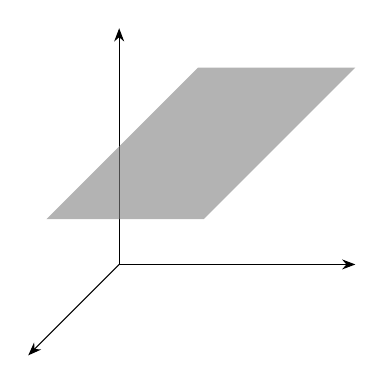
\begin{tikzpicture}[=>stealth]
\draw[-Stealth](0,0,0)--(0,0,3);
\draw[-Stealth](0,0,0)--(0,3,0);
\draw[-Stealth](0,0,0)--(3,0,0);
\path[fill=gray,opacity=0.6](1,2.5,0)--(3,2.5,0)--(3,2.5,5)--(1,2.5,5)--(1,2.5,0);
\end{tikzpicture}
\end{figure}


It is assumed that $Y$ is linearly related to $X_1$ and $X_2$.\\

$Y=\beta_0+\beta_1X_1+\beta_2X_2$ is a plane in $3-$ dimension.\\
$\beta_0=$ is the $y-$ intercept of the regression plane.\\

If the model includes $X_1=0$ and $X_2=0$, $\beta_0$ has particular meaning as a separate term in the regression model.\\

$\beta_1=$ Change in the  mean response of $Y$ per unit (increase) change in $X_1$ when $X_2$ is held constant.\\
$\beta_2=$ Change in the mean response of $Y$ per unit increase in $X_2$ when $X_1$ is held constant.\\


\begin{align*}
E\big(Y/X_1,X_2\big) & = \beta_0+\beta_1X_1+\beta_2X_2\\
\frac{\partial}{\partial X_1}E\big(Y/X_1,X_2\big) & = \beta_1\\
\frac{\partial}{\partial X_2}E\big(Y/X_1,X_2\big) & = \beta_2\\
\end{align*}

$Y=XB+\varepsilon$\\
$Y$ and $\varepsilon$ same as in simple linear regression
$$X=
\begin{pmatrix}
1 & X_{11} & X_{12}\\
1 & X_{21} & X_{22}\\
\vdots & \vdots & \vdots \\
1 & X_{n1} & X_{n2}\\
\end{pmatrix}
\,,\quad  B=
\begin{pmatrix}
\beta_0\\
\beta_1\\
\beta_2\\
\end{pmatrix}
$$


     
     
     
     
     
     
\subsection{General Multiple Line Regression}


\textbf{Introduction}\\
Multiple linear regression analysis is one of the most widely used of all statistical tools. The problem is estimating or predicting the values of a dependent variable $Y$ on the basis of a  set of  measurements taken on several independent variables $X_1,X_2,\ldots ,X_{k-1}$. For example we wish to estimate the speed of wind $(Y)$ as a function of height above ground $(X_1)$, temperature $(X_2)$ and pressure $(X_3)$. The predication  equation is obtained using least squares estimator on data collected at various heights temperatures and pressures to evaluate the necessary coefficients in the assumed model.
$$E\big(Y/X_1,X_2,X_3\big)=\beta_0+\beta_1X_1+\beta_2X_2+\beta_3X_3$$
$$Y=XB+\varepsilon,\quad  \varepsilon \thicksim N\big(0,\sigma^2 I_n\big)$$
$$Y_i=\beta_0+\beta_1X_{i1}+\beta_2X_{i2}+\beta_3X_{i3}+e_i\,,\quad  e_i\thicksim^{iid}N(0,\sigma^2)$$

Multiple linear regression models are often used as approximating function, relationship between $Y$ and $X_1,X_2,\ldots ,X_{k-1}$ is known, but over certain ranges of the regression variables $\big(X_1,X_2,\ldots ,X_{k-1}\big)$ the linear regression model is an adequate approximation.\\
Models that are complex is  structure then $$Y_i=\beta_0+\beta_1X_{i1}+\beta_2X_{i2}+\cdots + \beta_{k-1}X{ik-1}+e_{i1}$$ may still be analysed by linear regression techniques.\\

For example, a cubic polynomial model $$ Y=\beta_0+\beta_1X+\beta_2X^2+\beta_3X^3+e$$
Let $X_1=X,\quad  X_2=X$ and $X_3=X^3$ then we have  
$$Y=\beta_0+\beta_1X_1+\beta_2X_2+\beta_3X_3+e$$
we will generally write the multiple linear regression model $$Y_i=\beta_0+X_{i1}\beta_1+\cdots + X_{ik-1}\beta_{k-1}+e_i\quad  \text{as}\quad  Y_i=\sum^{k-1}_{j=0}X_{ij}\beta_j+e_j,\quad  X_{i0}=1,2,3\cdots ,n$$
$$E\big(Y/X\big)=\sum^{k-1}_{j=0}X_{ij}\beta_j$$
$$Y=XB+\varepsilon\,,\quad  B=\big(\beta_0,\beta_1,\ldots ,\beta_{k-1}\big)^t$$
$$X=
\begin{pmatrix}
1_n & X_1 & X_2 & \cdots & X_{k-1}\\
\end{pmatrix}
\,,\quad  X_j=
\begin{pmatrix}
X_{1j} & X_{2j} & X_{nj}\\
\end{pmatrix}^t,\quad 
j=1,2,\ldots ,k-1
$$\\


\subsection{Meaning of the Coefficients}
$$E\big(Y/X_1,X_2,\ldots ,X_{k-1}\big) = \sum^{k-1}_{j=0}\beta_jX_j$$
The parameter $\beta_0$ is the $Y$ intercept of the regression plane, it is the mean response at the origin. Though in certain situations $\beta_0$ has no practical importance. The parameter $\beta_j$ indicates change in the response variable $Y$ per unit increase in $X_j=\big(j=1,2,\ldots ,k-1\big)$ when the other variables are held constant. The regression model is a linear model, with design matrix having its columns as vectors of the independent variables
$$Y=XB+\varepsilon\quad  ,\quad  E(\varepsilon)=0$$
\begin{align*}
Cov(\varepsilon) & = \sigma^2I_n,\quad  \text{there}\quad  E(Y)=XB\\
Cov(Y) & = \sigma^2I\\
\end{align*} 


\begin{align*}
\big(X^tX\big)\widehat{B} & = X^tY\\
\implies \quad  \widehat{B} & = \big(X^tX\big)^{-1}X^tY\\
\widehat{Y}= X\widehat{B} & = X\big(X^tX\big)^{-1}X^tY=P_vY
\end{align*}
where $P_v=X\big(X^tX\big)^{-1}X^t$ is the projection matrix. we denote $P_v$ as $H$ $$\widehat{Y}=HY,\quad  H^t=H,\quad  \big(I-H\big)^2=I-H$$
$$\text{SST}=\sum^n_{i=1}\big(Y_i-\overline{Y}\big)^2=Y^t\Big(I-\frac{J_n}{n}\Big)Y$$
$$\frac{1_n1^t_n}{n}=\frac{J_n}{n}$$
\begin{align*}
\text{SSE} & = \sum^n_{i=1}\big(Y-\widehat{Y}\big)^2= \big(Y-\widehat{Y}\big)^t\big(Y-\widehat{Y}\big)\\
           & = Y^t\big(I-H\big)Y;\quad  H=X\big(X^tX\big)^{-1}X^t\\
           & = \quad \text{error sum of squares}\\
           & = \quad  \text{Residual sum of squares}
\end{align*}
\begin{align*}
\text{SSR} & = \quad  \text{Regression sum of squares}\\
\end{align*}
\begin{align*}
\text{SST} & = \text{SSR} + \text{SSE}\\
Y^t\Big(I-\frac{J_n}{n}\Big)Y & = \text{SSR} + Y^t(I-H)Y\\
\text{SSR} & = Y^t\Big(I-\frac{J_n}{n}\Big)Y-Y^t(I-H)Y\\
           & = Y^t\Big[I-\frac{J_n}{n}-I+H\Big]Y
\end{align*}
\begin{align*}
\text{SSR} & = \sum^n_{i=1}\big(\widehat{Y}_i-\overline{Y}\big)^2\\
           & = Y^t\Big(H-\frac{J_n}{n}\Big)Y\quad \text{Regression sum of squares}\\
Y_i-\overline{Y} & = \widehat{Y}_i-\overline{Y} + \big(Y_i-\widehat{Y}_i\big)\\
\text{SST} & = \text{SSR} + \text{SSE}\\
      n-1 & = (k-1) + (n-k)
\end{align*}


\begin{table}[H]
\centering
\textbf{ANOVA TABLE}\\
\begin{tabular}{|c|c|c|c|c|}
\hline
Source of & SS & df & MS & F\\
variation & & & &\\
\hline
Regression & SSR & $k-1$ & $\text{MSR}=\frac{\text{SSR}}{k-1}$ & $\frac{\text{MSR}}{\text{MSE}}\thicksim f_{k-1,n-k}$ \\
&&&& under $H_0$\\
&&&&\\
Error & SSE & $n-k$ & $\text{MSE}=\frac{\text{SSE}}{n-k}$ & $H_0:\beta_j=0$\\
(residual) &&&& $j=1,2,\ldots ,k-1$\\
&&&&\\
Total & SST & $n-1$ &&\\
\hline
\end{tabular}
\end{table}


$R^2=$ Coefficient of multiple determination.\\

$R^2=\frac{\text{SSR}}{\text{SST}}\quad $ Proportion of variation in $Y$ about $\overline{Y}$ explained by the regression model
\begin{align*}
R^2 & = \frac{\text{SSR}}{\text{SST}}\\
    & = 1-\frac{\text{SSE}}{\text{SST}}
\end{align*}
$R^2=1-$ Proportion of variation in $Y$ about $\overline{Y}$ unexplained by the regression model.\\


Alternatively $R^2$ is the proportionate reduction of the total variation in $Y$ about $\overline{Y}$ associated with the set of variables $X_1,X_2,\ldots , X_{k-1}$.\\

$R^2=0$, if $\hat{\beta}_j=0,\quad  j=1,2,\ldots ,k-1$.\\

$R^2=1$, when there is a perfect fit. i.e all the $Y_i's$ lie on the regression surface.\\

However, adding more independent (regression) variables to model can only increase $R^2$ because SSE can never become larger with more independent variables.\\
Hence, the need for adjusting $R^2$ to recognise the number of independent variables in model 
\begin{align*}
R^2_a & = 1-\frac{\text{SSE}/(n-k)}{\text{SST}/(n-1)}=1-\frac{\text{MSE}}{\text{MST}}\\
      & = \,\text{adjusted coefficients of multiple determination}\\
\end{align*}


Full model: $Y_i=\beta_0+\beta_1X_{i1}+\beta_2X_{i2}+\beta_4X_{i4}+e_i\quad  i=1,2,\ldots ,n$
$$\text{SST} = \text{SSR} + \text{SSE}\quad  R^2_4=1-\frac{\text{MSE}}{\text{MST}}$$
$$Y_i=\beta_0+\beta_1X_{i1}+\beta_3X_{i3}+\beta_4X_{i4}+e_i\quad  i=1,2,\ldots ,n$$
$$\text{SST} = \text{SSR}(X_2) +\text{SSE}(X_2)$$
$$R^2_a(X_2)=1-\frac{\text{MSE}(X_2)}{\text{MST}}$$
$$R^2_a<R^2_a(X_2)$$\\


SST $=$ SSR $+$ SSE
$$Y=\sum_{j=0}X_j\beta_j+e\qquad  Y_i=\sum_{j=0}X_{ij}\beta_j+e_i\quad  i=1,2,\ldots ,n$$

SST $=$ Total sum of squares\\
SSR $=$ Regression sum of  squares.
SSE $=$ Residual (error) sum of squares.

If we have the model $Y=\beta_0+x_1\beta_1+x_2\beta_2+x_3\beta_3+e$\\
SST $=$ SSR$\big(X_1,X_2,X_3\big)$ $+$ SSE$\big(X_1,X_2,X_3\big)$\\


If the model is $Y=\beta_0+x_2\beta_2+x_3\beta_3+e$ then \\
SST $=$ SSR$\big(X_2,X_3\big)$ + SSE$\big(X_2,X_3\big)$\\

\begin{note}
\begin{itemize}
      \item[] SSR$\big(X_2,X_3\big)<$ SSR$\big(X_1,X_2,X_3\big)$
      
      \item[] SSE$\big(X_2,X_3\big) >$ SSE$\big(X_1,X_2,X_3\big)$\\
\end{itemize}


If the model is $Y=\beta_0+\beta_1X_1+\beta_2X_2+e$\\

SST = SSR$\big(X_1,X_2\big)$ + SSE$\big(X_1,X_2\big)$\\

SSR$\big(X_1,X_2\big)<$ SSR$\big(X_1,X_2,X_3\big)$ and SSE$\big(X_1,X_2\big)>$ SSE$\big(X_1,X_2,X_3\big)$.\\


SSE$\big(X_1/X_2\big)=$ Reduction of SSE when $X_1$ is introduced given that $X_2$ is already in model.\\

SSE$\big(X_2/X_1\big)=$ SSE$(X_1)-$ SSE$\big(X_1,X_2\big)$.\\

SSE$\big(X_3/X_1,X_2\big)=$ SSE$\big(X_1,X_2\big)-$ SSE$\big(X_1,X_2,X_3\big)$\\

Reduction in the SSE when $X_3$ is introduced given that $X_1$ and $X_2$ are in model\\

SSE$\big(X_2,X_1/X_3)=$ SSE$\big(X_3\big)-$ SSE$\big(X_1,X_2,X_3\big)$\\

$X_1$ (first) $\qquad  X_3$(second) $\qquad  X_2$(third)\\

\begin{align*}
\text{SSR}\big(X_3/X_1\big) & = \text{SSE}\big(X_1\big)-\text{SSE}\big(X_1,X_3\big)\\
                            & = \text{SST}-\text{SSR}\big(X_1\big)-\Big(\text{SST}-\text{SSR}\big(X_1,X_3\big)\Big)\\
\text{SSR}\big(X_3/X_1\big) & = \text{SSR}\big(X_1,X_3\big)-\text{SSR}\big(X_1\big)\quad \cdots \, (a)
\end{align*}

increase of the SSR when $X_3$ is introduced given that $X_1$ is already in the model

$$\text{SSR}\big(X_2/X_1,X_3\big)=\text{SSR}\big(X_1,X_2,X_3\big)-\text{SSR}\big(X_1,X_3\big)\quad \cdots \quad  (b)$$
increase of the SSR when $X_2$ is introduced given that $X_1$ and $X_3$ is already in the model


\begin{align*}
\underbrace{\text{SST}}_{n-1} & = \underbrace{\text{SSR}\big(X_1,X_2,X_3\big)}_3+\underbrace{\text{SSE}\big(X_1,X_2,X_3\big)}_{n-4}\\
                              & = \text{SSR}\big(X_2/X_1,X_3\big)+\text{SSR}\big(X_1,X_3\big)+\text{SSE}\big(X_1,X_2,X_3\big)\quad  \text{from}\quad  (b)\\
                              & = \text{SSR}\big(X_2/X_1,X_3\big)+\text{SSR}\big(X_3/X_2\big)+\text{SSR}\big(X_1\big)+\text{SSE}\big(X_1,X_2,X_3\big)\quad \text{from}\quad  (a)\\
            \text{SST} & = \text{SSR}\big(X_1\big)+\text{SSR}\big(X_3/X_1\big)+\text{SSR}\big(X_2/X_1,X_3\big)+\text{SSE}\big(X_1,X_2,X_3\big)
\end{align*}


\begin{table}[H]
\centering
\textbf{ANOVA}\\
\begin{tabular}{|c|c|c|c|c|}
\hline
Source of & SS & df & MS & F\\
Variation &    &    &    &\\
\hline
&&&&\\
Regression & SSR$\big(X_1,X_2,X_3\big)$ & 3 & MSR$\big(X_1,X_2,X_3\big)$ & $H_0:\beta_j=0,\quad  j=1,2,3$\\
&&&&\\
$X_1$ & SSR$(X_1)$ & 1 & MSR$(X_1)$ & $H_0:\beta_1=0$ \\
&&&&\\
$X_3/X_1$ & SSR$(X_3/X_1)$ & 1 & MSR$(X_3/X_1)$ & do we need $X_3$ given $X_1$ \\
&&&& is already in the model\\
&&&&\\
&&&&\\
$X_2/X_1,X_3$ & SSR$(X_2/X_1,X_3$ & 1 & MSR$(X_2/X_1,X_3)$ & do we need $X_2$ given $X_1$ and $X_3$\\
&&&& is already in the model\\
&&&&\\
Error & SSE$(X_1,X_2,X_3)$ & $n-4$ & MSE$(X_1,X_2,X_3)$ &\\
&&&&\\
Total & SST & $n-1$ &&\\
\hline
\end{tabular}
\end{table}

First $(X_2)$ $\quad $, second $(X_1$ and $X_3)$
$$\text{SSR}\big(X_1,X_2,X_3\big) = \text{SSR}\big(X_2\big) + \text{SSR}\big(X_1,X_3/X_2\big)$$
\end{note}


\begin{exa}
\begin{enumerate}
\item The department of Fisheries (DOF) wants to estimate the number of breams caught in some lakes in order to restock the lakes with appropriate number of fingerling (body fish). The DOF samples and record $Y_1$ the seasonal catch per square Km of lake area, $X_1$, the number of lake shore  residents per square Km, $X_2$, the size of the lake in square Km, $X_3=1$, if the lake has public access, 0 if not, and $X_4$, a structure index. Twenty random samples were taken, the fitted model $$Y=-2.78+0.0268X_1+0.504X_2+0.743X_3+0.0511X_4$$
\begin{enumerate}
     \item Complete the ANOVA TABLE and test for significance of the model
\begin{table}[H]
\centering
\begin{tabular}{|c|c|c|c|c|}
\hline
Source & SS & df & MS & F\\
\hline
&&&&\\
Regression & 24.0624 & 4 & 6.0156 & 39.655$\thicksim f_{4,15}^{0.05}$\\
&&&&\\
Error & 2.2756 & 15 & 0.1517 &\\
&&&&\\
\hline
&&&&\\
Total & 26.338 & 19 & 1.386 &\\
\hline
\end{tabular}
\end{table}


    \item Compute the unadjusted coefficients  of multiple determination.
    
    \item The DOF is uncertain whether access $(X_3)$ and structure $(X_4)$ are useful as additional independent variables. A model was fit on the same data with only $X_1$ and $X_2$ and the regression sum of squares was 12.913. Are $X_3$ and $X_4$ useful additional predictors for estimating the number of breams caught.\\
\end{enumerate}

\begin{solution}
\begin{enumerate}
      \item 
\begin{align*}
R^2  & = \frac{\text{SSR}}{\text{SST}}=1-\frac{\text{SSE}}{\text{SST}}\\
     & = \frac{24.0624}{26.338}=1-\frac{2.2656}{26.338}\\
     & = 0.9136\\ \\
R^2_a & = 1-\frac{\text{MSE}}{\text{MST}}\\
      & = 1-\frac{0.1517}{1.386}\\
      & = 0.891\\
\end{align*}
$$ \text{adjusted}\qquad  R^2=\frac{\text{SSR}}{\text{SST}}=\frac{12.913}{26.336}$$
$$R^2_a=1-\frac{(26.38-12.913)/17}{1.386}=0.43$$\\

    \item SSR$\big(X_3,X_4/X_1,X_2\big)=$ SSR$\big(X_1,X_2,X_3,X_4\big)-$ SSR$(X_1,X_2)$\\
    
\begin{table}[H]
\centering
\begin{tabular}{|c|c|c|c|c|}
\hline
Source & SS & df & MS & F\\
\hline
&&&&\\ 
Regression & 24.0624 & 4 & &\\
&&&&\\
$X_1,X_2$ & 12.913 & 2 & &\\
&&&&\\
$X_3,X_4/X_1,X_2$ & 11.1494 & 2 & $\frac{11.1404}{2}$ & $F\thicksim f_{2,15}$\\
&&&&\\
Error & 2.2756 & 15 & 0.1517 & \\
&&&&\\
\hline
&&&&\\
Total & 26.338 & 19 & &\\
\hline
\end{tabular}
\end{table}   
We need the $X_3$ and $X_4$.\\ 
\end{enumerate}
\end{solution}


\item The heat evolved in Calories per gram of cement$(Y)$ as a function of each of four ingredients in the mix, aluminate $(X_1)$, silicate $(X_2)$, alumino-ferrite $(X_3)$ and dicalcium $(X_4)$, hence the following model:$$Y=\beta_0+\beta_1X_1+\beta_2X_2+\beta_3X_3+\beta_4X_4+e.$$ The fitted model on thirteen batches is $$\widehat{Y}=62.41+1.55X_1+0.51X_2+0.20X_3-0.14X_4$$

\begin{enumerate}
     \item Complete the ANOVA TABLE\\
     
\begin{table}[H]
\centering
\begin{tabular}{|c|c|c|c|c|}
\hline
Source & SS & df & MS & F\\
\hline
&&&&\\
Regression & 2667.90 & 4 & 667.0 & 111.5\\
&&&&\\
Residual & 47.86 & 8 & 5.983 & \\
\hline
&&&&\\
Total & 2715.76 & 12 & 226.3 & \\
\hline
\end{tabular}
\end{table}     
   
   \item Compute $R^2$ and $R^2_a$.\\
   
   \item What are the interpretations of the coefficients of $X_2$ and $X_4$?\\
   
   $\implies ($ the evolved increases by 0.51 per unit silicate)\\    
\end{enumerate}


\item For the model in (2) above, the reduced models with their SSR are given as follow 
\begin{table}[H]
\centering
\begin{tabular}{ll}
Model                                         & SSR\\
\hline
&\\
$Y=\beta_0+\beta_4X_4+e$                      & 1831.90\\
&\\
$Y=\beta_0+\beta_1X_1+\beta_2X_2+e$            & 2641.00\\
&\\
$Y=\beta_0+\beta_1X_1+\beta_4X_4+e$            & 2657.86\\
&\\
$Y=\beta_0+\beta_1X_1+\beta_2X_2+\beta_4X_4+e$ & 2667.79\\
&\\
\end{tabular}
\end{table}


\begin{enumerate}
       \item Compute $R^2$ and $R^2_a$ for $$Y=\beta_0+\beta_1X_1+\beta_4X_4+e$$
       \item Decompose the SSR for the model
       \item Test whether $X_2$ and $X_3$ are needed in the model which already has $X_1$ and $X_4$.\\
\end{enumerate}





\begin{solution}
\begin{enumerate}
\item The model in $X_1$ and $X_4$ has $\text{SSR}=2657.86$, and $\text{SST}$
does not depend on which model is fitted, so $\text{SST}=2715.76$ with
$n-1=12$ degrees of freedom and $n=13$. Hence
$$\text{SSE}=2715.76-2657.86=57.90, \qquad n-k=13-3=10,$$
$$R^{2}=\frac{2657.86}{2715.76}=0.9787,$$
$$R^{2}_{a}=1-\frac{\text{SSE}/(n-k)}{\text{SST}/(n-1)}
=1-\frac{57.90/10}{2715.76/12}=1-\frac{5.790}{226.31}=0.9744.$$
The full four-variable model gave $R^{2}=2667.90/2715.76=0.9824$. Dropping
$X_2$ and $X_3$ costs 0.0037 of $R^{2}$ and \emph{raises} the adjusted value,
which is the first sign of what part (c) confirms.

\item Each line is the extra regression sum of squares brought by a variable
given those above it, so the entries add to the regression sum of squares of
the full model.

\begin{table}[H]
\centering
\begin{tabular}{|l|c|c|}
\hline
\textbf{Source} & \textbf{SS} & \textbf{d.f.}\\
\hline
$X_4$ & 1831.90 & 1\\
$X_1\mid X_4$ & 825.96 & 1\\
$X_2\mid X_1,X_4$ & 9.93 & 1\\
$X_3\mid X_1,X_2,X_4$ & 0.11 & 1\\
\hline
$X_1,X_2,X_3,X_4$ & 2667.90 & 4\\
\hline
\end{tabular}
\caption{Sequential decomposition of the regression sum of squares. The four
extra sums of squares total $1831.90+825.96+9.93+0.11=2667.90$, which is the
regression sum of squares of the full model.}
\label{tab:seqssr}
\end{table}

\item The two variables are tested together, against the model that already
contains $X_1$ and $X_4$:
$$\text{SSR}\big(X_2,X_3\mid X_1,X_4\big)
=\text{SSR}\big(X_1,X_2,X_3,X_4\big)-\text{SSR}\big(X_1,X_4\big)
=2667.90-2657.86=10.04,$$
on $2$ degrees of freedom. With the full model's $\text{MSE}=5.983$,
$$F=\frac{\text{SSR}\big(X_2,X_3\mid X_1,X_4\big)/2}{\text{MSE}}
=\frac{10.04/2}{5.983}=0.84,$$
to be compared with $F_{2,8,0.05}=4.46$. Since $0.84<4.46$ the hypothesis
$\beta_2=\beta_3=0$ is not rejected: $X_2$ and $X_3$ are not needed once $X_1$
and $X_4$ are in the model.
\end{enumerate}

\begin{note}
The conclusion is about $X_2$ and $X_3$ \emph{jointly, and given $X_1$ and
$X_4$}. It does not say either variable is unrelated to $Y$: fitted alone,
$X_2$ explains a great deal. What the test says is that whatever they carry is
already carried by $X_1$ and $X_4$. This is why the decomposition of part (b)
is written as a sequence --- change the order of entry and the individual
lines change, though their total does not.
\end{note}
\end{solution}
\end{enumerate}
\end{exa}


\subsection{Multicollinearity}
Recall that $Y=XB+\varepsilon$, where the columns of $X$ are "independent" or regression variables when the columns of $X$ are orthogonal then $X^tX$ is a diagonal matrix. Unfortunately in most multiple regression applications the columns of $X$ are not orthogonal in some cases when the column of $X$ are not orthogonal there can be serious problems when there is near dependency between the independent variables columns of $X$ matrix the problem of multi Id linearity is said to exist: $X^t$ is about singular i.e $\det\big(X^tX\big)\approx 0$.\\

Let $X^*=$ the matrix in which the column have been centered and standardized.
$$X^*_{ij}=\frac{X_{ij}-\overline{X}_j}{\sqrt{S^2_j}}\,,  \quad  S^2_j=\sum^n_{j=1}\big(X_{ij}-\overline{X}_j\big)^2$$

diagonal $X_j^{*t}X^{*}_j=\frac{\sum\limits^n_{j=1}\big(X_{ij}-\overline{X}_{. j}\big)^2}{S^2_j}=1$ \\

off diagonal 
\begin{align*}
X^{*}_jX^*_{j'} & = \frac{\sum\limits^n_{i=1}\big(X_{ij}-\overline{X}_{.j}\big)\big(X_{ij'}-\overline{X}_{.j'}\big)}{S_jS_{j'}}\\
                & = \frac{\sum\big(X_{ij}-\overline{X}_{.j}\big)\big(X_{ij'}-\overline{X}_{.j'}\big)}{\sqrt{\sum \big(X_{ij}-\overline{X}_{.j}\big)^2\sum\big(X_{ij'}-\overline{X}_{.j'}\big)^2}}
\end{align*}


\begin{solution}
\begin{enumerate}
\item[]
\begin{enumerate}
\item[b).]
\begin{enumerate}
       \item table
       \item $R^2=1-\frac{\text{SSE}}{\text{SST}}=1-\frac{47.86}{2715.76}=0.9824$\\
       
       $R^2_a=1-\frac{\text{MSE}}{\text{MST}}=1-\frac{5.983}{226.3}=0.9736$\\
       
       \item heat evolved increase by 0.51 per unit increase in silicate.\\
       heat evolved reduces by 0.41 per unit reduction in dicalcium.\\
\end{enumerate}


\item[c).]
\begin{enumerate}
         \item $R^2=\frac{\text{SSR}}{\text{SST}}=\frac{2657.86}{2715.76}=0.978$\\
         
\begin{table}[H]
\centering
\begin{tabular}{|c|c|c|c|}
\hline
Source & SS & df & MS\\
\hline
&&&\\
Regression & 2657.86 & 2 & 1328.9\\
&&&\\
Error & 57.9 & 10 & 5.79\\
&&&\\
Total & 2715.76 & 12 & 226.3\\
\hline
\end{tabular}
\end{table}

$$R^2_a=1-\frac{\text{MSE}}{\text{MST}}=1-\frac{5.79}{226.3}=0.974$$\\

       \item table\\
       
       
       \item\quad 
\begin{table}[H]
\centering
\begin{tabular}{|c|c|c|c|c|}
\hline
Source & SS & df & MS & F\\
\hline
Regression & 2667.96 & 4 & &\\
&&&&\\
$X_1,X_4$ & 2657.86 & 2 & & \\
&&&&\\
$X_2,X_3/X_1,X_4$ & 10.04 & 2 & 5.02 & 0.84\\
&&&&\\
Error & 47.86 & 8 & 5.98 &\\
&&&&\\
Total & 2715.76 & 12 & &\\
\hline
\end{tabular}
\end{table}

$$F^{0.05}_{2,8}=4.459$$

$\therefore$ We do not need $X_2$ and $X_3$.\\
\end{enumerate}
\end{enumerate}
\end{enumerate}
\end{solution}


$X^{*t}X^*$ the main diagonal elements are  ones and the off diagonal elements are correlation coefficients i.e $\big(j,j'\big)^{\text{th}}$ element $\big(j\neq j'\big)$ is $X_{ij}=$ correlation coefficients  are "large" then there might be a problem. If $X_j$ and $X_{j'}$ are nearly dependent the $|X_{ij}|$ $|X_{ij'}|$ will be near unity (one).


A different way of examining multicollinearity is finding the eigenvalues of $X^tX[|X^tX-\lambda I|]=0$ (characteristic roots).\\

The eigenvalues of $X^tX$ say $\lambda_1,\lambda_2,\ldots ,\lambda_k$ can be used to measure the extent of collinearity.\\

Let $\lambda_{\max}=\max\{\lambda_1,\lambda_2,\ldots ,\lambda_k\}$ and $\lambda_{\min}=\min\{\lambda_1,\lambda_2,\ldots ,\lambda_k\}$ then the ratio $\frac{\lambda_{\max}}{\lambda_{\min}}$ is known as the condition number if the condition number
\begin{table}[H]
\centering
\begin{tabular}{|c|l|}
\hline
\textbf{Condition number} & \textbf{Interpretation}\\
\hline
$<100$ & No serious problem of multicollinearity\\
$100$ to $1{,}000$ & Moderate multicollinearity\\
$>1{,}000$ & Serious or severe multicollinearity\\
\hline
\end{tabular}
\caption{Conventional reading of the condition number
$\lambda_{\max}/\lambda_{\min}$. The boundaries are rules of thumb, not test
critical values: nothing changes abruptly at $100$.}
\label{tab:conditionnumber}
\end{table}

$$
\begin{pmatrix}
n_1 & 0 & 0\\
0 & n_2 & 0\\
0 & 0 & n_3\\
\end{pmatrix}
$$
\begin{align*}
\Big|X^tX-\lambda I_3\Big| & = 
\begin{vmatrix}
n_1-\lambda & 0 & 0\\
0 & n_2-\lambda & 0\\
0 & 0 & n_3-\lambda\\
\end{vmatrix}
=0\\
                          & = \big(n_1-\lambda\big)\big(n_2-\lambda\big)\big(n_3-\lambda\big)=0
\end{align*}
$$\implies \quad  \lambda_1= n_1,\quad  \lambda_2=n_2,\quad  \lambda_3=n_3$$\\

Why should we be concerned about collinearity?\\

Recall that $\widehat{B}=\big(X^tX\big)^{-1}X^tY$ and $\quad  Cov\big(\widehat{B}\big)=\big(X^tX\big)^{-1}\sigma^2$.\\

The least squares estimation produces estimated regression coefficients that are too large in absolute value.\\

There are a number of methods of dealing with collinearity.
\begin{itemize}
\item Collecting additional data
\item Model respecification
\item Ridge regression, $\big(X^tX+\alpha I\big)\widehat{B}_n=X^tY$ $\{$ becomes your normal equations $\}$
\item Generalized ridge regression
\item Principal component regression $$Y=Z\alpha + \varepsilon,\quad  Z=XT,$$ where $T$ is the matrix whose columns are the eigenvectors of $\lambda_1,\lambda_2,\ldots ,\lambda_k$.
\item Latent root regression analysis.\\
\end{itemize}


\subsection{Examination of Residuals(errors)}
The residuals are defined as $n$ differences $$\widehat{e}_i=Y_i-\widehat{Y}_i,\quad  i=1,2,\ldots ,n$$ 
$$\widehat{Y}_i=\sum^{k-1}_{j=0}X_{ij}\widehat{B}_j$$
In performing the regression analysis we make certain assumptions about the errors
\begin{enumerate}
\item Constant variance
\item Normal distribution  $\quad  \varepsilon \thicksim^{iid}N(0,\sigma^2)$
\item Independent 
\end{enumerate}

If our fitted model is "correct" the residuals should exhibit tendencies that conform to the assumptions.\\

After examining the residuals we must conclude that either the assumptions appear to be violated or the assumptions do not appear to be violated.\\

The ways of examining the residuals we will discuss are all graphical the graphical ways are easy to do are usually very revealing when assumptions are violated.\\

The four principal way of plotting the residuals are
\begin{enumerate}
\item[]
\begin{enumerate}
       \item Overall plot (scatter diagram)
       \item In time sequence if order is known
       \item Against the fitted values $\big(\widehat{Y}$ vs $\widehat{e}\big)$
       $$\widehat{Y}=X\widehat{B}\implies \widehat{e}=Y-\widehat{Y}=Y-X\widehat{B}$$
\begin{align*}
\widehat{e} & = Y-X\big(X^tX\big)^{-1}X^tY\\
        & = \big(I-H\big)Y\quad  \text{where}\quad  H=X\big(X^tX\big)^{-1}X^t\quad  \text{Hessian matrix}
\end{align*}

       \item Against the independent variables $\big(X_j$ vs $\widehat{e}\big)$\\
\end{enumerate}
\end{enumerate}


In addition to the above four the residuals should be also plotted in anyway that is sensible for a particular problem under consideration.\\

The standardized residuals $\frac{\widehat{e}}{\sqrt{1-h_{ii}}}$, $\quad  h_{ii}$ is the $i^{\text{th}}$ diagonal elements of the Hessian matrix $H$
\begin{align*}
\widehat{e}=\big(I-H\big)Y,\quad  Cov\big(\widehat{e}\big) & = \big(I-H\big)Cov\big(Y\big)\big(I-H\big)^t\\
                                                           & = \big(I-H\big)I\sigma^2\big(I-H\big)^t\\
                                                           & = \big(I-H\big)\sigma^2
\end{align*}
An alternative procedure is to construct a normal plot or half normal plot.\\

The points should fall approximately on a straight line

% DIAGRAM 6
\begin{figure}[H]
\centering
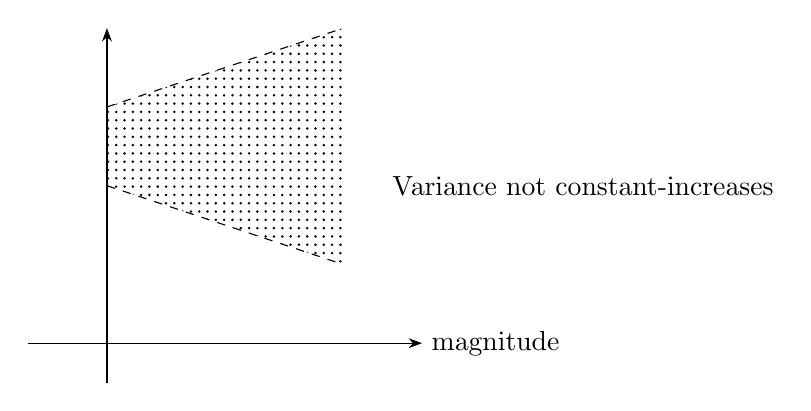
\begin{tikzpicture}[=>stealth]
\draw[-Stealth](-1,0)--(4,0)node[right]{magnitude};
\draw[-Stealth](0,-0.5)--(0,4);
\draw[dashed](0,2)--(3,1)
(0,3)--(3,4);
\path[pattern=dots](3,4)--(0,3)--(0,2)--(3,1);
\draw(3.5,2)node[right]{Variance not constant-increases};
\end{tikzpicture}\\
\end{figure}
 
 


% DIAGRAM 7
\begin{figure}[H]
\centering
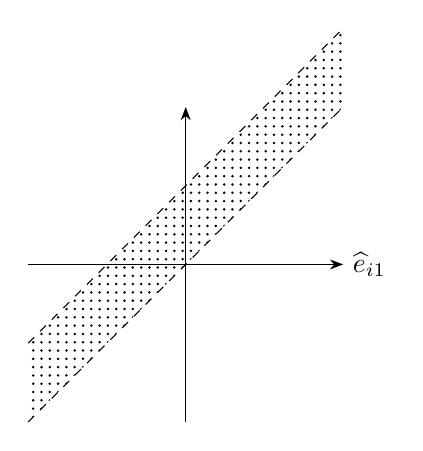
\begin{tikzpicture}[=>stealth]
\draw[-Stealth](-2,0)--(2,0)node[right]{$\widehat{e}_{i1}$};
\draw[-Stealth](0,-2)--(0,2);
\path[pattern=dots,dashed,shape=rectangle](2,3)--(-1,0)--(0,0)--(2,2);
\path[pattern=dots,dashed,shape=rectangle](-2,-1)--(-1,0)--(0,0)--(-2,-2);
\draw[dashed](-2,-1)--(2,3) 
(-2,-2)--(2,2);
\end{tikzpicture}
\end{figure}


Linear term must be included in the model\\


% DIAGRAM 8

\begin{figure}[H]
\centering
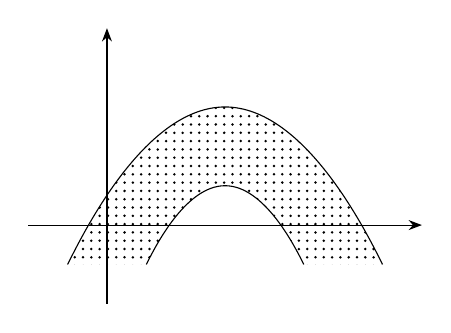
\begin{tikzpicture}[=>stealth]
\draw[-Stealth](-2.5,0.5)--(2.5,0.5);
\draw[-Stealth](-1.5,-0.5)--(-1.5,3);
\draw(0,2)parabola(-2,0)
(0,2)parabola(2,0)
(0,1)parabola(-1,0)
(0,1)parabola(1,0);
\path[pattern =dots](-2,0)parabola[bend at end](0,2)--(0,2)parabola(2,0)--(1,0)parabola[bend at end](0,1)--(0,1)parabola(-1,0)--(-2,0)--cycle;
\end{tikzpicture}
\end{figure}


\begin{itemize}
\item Linear and Quadratic term should be included
\item Need extra terms
\item Model transformation of $Y_i's$
\item Cross product terms 
$$\text{i.e}\quad  X_jX_{j'}$$ $$\beta_0+\beta_1x_1+\beta_2x_2+\beta_3x_1x_2+e$$

$f_i=\frac{\widehat{e}_i}{\sqrt{\text{MSE}-\big(I-h_{ii}\big)}}\quad $ are known as standardized residuals.\\

$\frac{\widehat{e}_i}{\sqrt{I-h_{ii}}}$ are known as standardized residuals.\\
\end{itemize}


\subsection{Hazards in the use of Regression}
Regression analysis is widely used and unfortunately if frequently misused.\\

There are several common abuses on linear regression that should be mentioned
\begin{enumerate}
\item Linear regression model may not be valid for extra plotion outside a certain range.

%  DIAGRAM 9
\begin{figure}[H]
\centering
\begin{tikzpicture}[=>stealth]
\draw[-Stealth]
(0,-1.5)--(0,3)node[above]{$Y$};
\draw[smooth,scale=0.5,domain=0.7:7, variable=\x]plot(\x,{1+2*sin((2*\x)r)});
\draw[smooth,domain=-0.5:4,variable=\x]plot(\x,{1/2*\x})node[right]{$\widehat{Y} =\widehat{\beta}_0 + \widehat{\beta}_1X$};
\draw[-Stealth](-0.5,-1)--(4,-1)node[right]{$X$};
\end{tikzpicture}
\end{figure}





\item Influential points

% DIAGRAM 10
\begin{figure}[H]
\centering
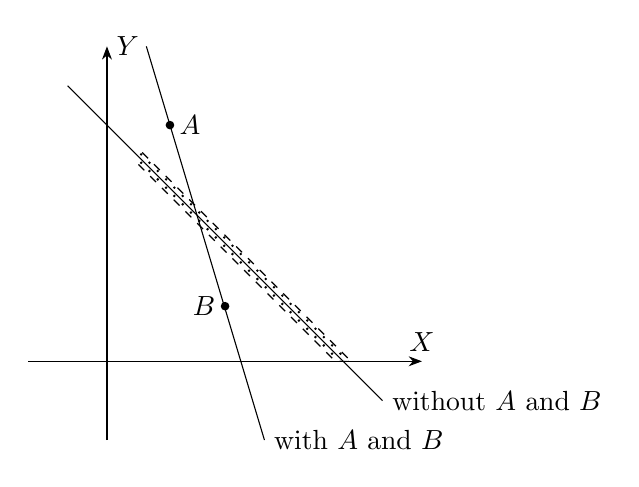
\begin{tikzpicture}[=>stealth]
\draw[-Stealth](-1,0)--(4,0)node[above]{$X$};
\draw[-Stealth](0,-1)--(0,4)node[right]{$Y$};
\draw(0.5,4)--(2,-1)node[right]{with $A$ and $B$};
\draw[smooth,domain=-0.5:3.5,variable=\x]plot({\x},{-\x+3})node[right]{without $A$ and $B$};
\draw[dashed,pattern=dots](0.4,2.5)--(2.9,0)--(3.1,0)--(0.4,2.7);
\draw(1.5,0.7)node[shape=circle,draw,scale=0.01cm,fill=black]{};
\draw(0.8,3)node[shape=circle,draw,scale=0.01cm,fill=black]{};
\draw(0.8,3)node[right]{$A$}
(1.5,0.7)node[left]{$B$};
\end{tikzpicture}\\
$A$ and $B$ are known as influential points\\
\end{figure}


\item Outlies or "bad" values (points)

% DIAGRAM 11
\begin{figure}[H]
\centering
\begin{tikzpicture}[=>stealth]
\draw[-Stealth](-1,0)--(4,0);
\draw[-Stealth](0,-1)--(0,4);
\draw[smooth,domain=0.5:4,variable=\x]plot(\x,\x)node[right]{$\widehat{Y}=\widehat{\beta}_0+\widehat{\beta}_1X$ without d};
\filldraw[pattern=dots,dashed,shape=rectangle](3,2.5)--(1,0.5)--(1,1.5)--(3,3.5);
\draw(1,2)node[shape=circle,draw,scale=0.01cm,fill=black]{};
\draw(1,2)node[above]{d};
\end{tikzpicture}
\end{figure}


\item Just because a regression analysis has indicated a strong relationship between $Y$ and $X$ doesn't imply that the variables are related in any casual sense.
\begin{align*}
Y & = \quad \text{number of certified mental patients per 10,000 estimated populations}\\
X_1 & = \quad \text{number of radio station lincenses issued in UK}\\
X_2 & = \quad \text{first name of president of the U.S.A}
\end{align*}
$(1924-1937) $  Kendall and Yule 

\begin{align*}
\widehat{Y} & = 4.582+2.204X_1, \quad  R^2=0.9842\\
H_0: \beta_1 & =0,\quad  t_{cal}=27.312
\end{align*}
\begin{align*}
\widehat{Y} & = -26.442+5.900X_2,\quad  R^2=0.8709\\
H_0: \beta_2 &=0,\quad  t_{cal}=8.996\\
\end{align*}
Both equations  give nonsense relationship.

\item In some applications of regression the values of the independent variable required for the predication of $Y$ is unknown.\\

\begin{exa}
Consider predicting maximum daily load on an electric power generation system from regression model relating the load to maximum daily temperature.
\end{exa}

\end{enumerate}


\pagebreak

\thispagestyle{empty}


\textbf{LINEAR MODELS AND DESIGN OF EXPERIMENTS}\\


\textbf{Pre-requisites:} \, M212-Mathematical Methods, M222- Linear algebra and M261 - Introduction to Statistics

\begin{itemize}
\item[]\textbf{Random vectors and Random matrices}\\
Expectation vector. Variance - covariance matrices. Distribution of a linear transformation.

\item[]\textbf{Multiple Regression}\\
Multiple Regression model. Least squares estimators and their statistical properties Residual Analysis. Weighted least squares estimators. Test of general  linear hypothesis. Multi -collinearity

\item[]\textbf{Analysis of variance}\\
Estimation and multiple comparison. Three way Analysis of Variance. Experimental Designs: Completely Randomized Design, Randomized Block Design, Latin Square Design.

\item[]\textbf{Analysis of Covariance}\\
One way classification with one covariate. One way classification with two covariates. Development by the general regression significant test.\\
\end{itemize}


\textbf{Prescribed Textbooks}
\begin{enumerate}
\item Applied statistics. Dunn, O. and Clark, V. 1987. John Wiley.
\item Introduction to linear regression analysis. Montgonomory, D. and Peck, E. 1982. John Wiley.\\
\end{enumerate}


\textbf{Recommended Textbooks}

\begin{enumerate}
\item[3.] Applied Statistical Linear Models. Neter, J. and Wasserman 1974. Richard D. Irwin, Inc.
\item[4.] Design and analysis of experiments. Montgomery, D. 1984. John Wiley.
\end{enumerate}


\end{document}